\documentclass[11pt,a4paper]{article}
%%% \usepackage{mathptm,times}
%%%  \usepackage[pdftex]{graphicx}
% \usepackage{hyperref}
%
\usepackage[T1]{fontenc}
\usepackage[latin1]{inputenc}
\usepackage[english]{babel}
\usepackage{fancyhdr}
\usepackage{upquote}
% upquote toimii vain verbatimissa. \char"0D antaa muualla
% oikeanlaisen hipsun.

%\usepackage{eso-pic}
\usepackage[dvips]{graphicx}
%\usepackage{graphicx}
%\usepackage{ae,aecompl} 
\usepackage{times} 
\usepackage{amsmath}
\usepackage{amssymb,amsfonts}
%\usepackage{color}
%\usepackage{type1cm}

%\makeatletter 
%   \AddToShipoutPicture{%
%     \setlength{\@tempdimb}{.5\paperwidth}%
%    \setlength{\@tempdimc}{.5\paperheight}%
%   \setlength{\unitlength}{1pt}%
%  \put(\strip@pt\@tempdimb,\strip@pt\@tempdimc){%
%     \makebox(0,0){\rotatebox{45}{\textcolor[gray]{0.75}{
%     \fontsize{8cm}{8cm}\selectfont{DRAFT}}}}}} 
%\makeatother

\setlength{\textwidth}{6.5in}
\setlength{\textheight}{9.0in}
\setlength{\topmargin}{0.in}
\setlength{\headheight}{0.in}
\setlength{\headsep}{0.in}
\setlength{\parindent}{0.25in}
\setlength{\oddsidemargin}{0.0in}
\setlength{\evensidemargin}{0.0in}


\pagestyle{plain}

\begin{document}

% \bibliographystyle{unsrt}

%% \newcommand{\dod}[2]{\frac{\partial #1}{\partial #2}}
%% \newcommand{\DoD}[2]{\frac{D #1}{D #2}}
%% \newcommand{\dsods}[2]{\frac{\partial^2 #1}{\partial #2^2}}
%% \newcommand{\dx}{\delta x}
%% \newcommand{\dy}{\delta y}
%% \newcommand{\dz}{\delta z}
%% \newcommand{\x}{x}
%% \newcommand{\y}{y}
%% \newcommand{\z}{z}
%% \newcommand{\dt}{\delta t}
%% \newcommand{\dn}{\delta n}
%% \newcommand{\hu}{u}
%% \newcommand{\hv}{v}
%% \newcommand{\hw}{w}
%% \newcommand{\la}{\lambda}
%% %\newcommand{\bO}{\mbox{\boldmath $\Omega$}}
%% \newcommand{\bO}{{\Omega}}
%% \newcommand{\bo}{{\bf \omega}}
%% %\newcommand{\btau}{\mbox{\boldmath $\tau$}}
%% \newcommand{\btau}{{\bf \tau}}
%% \newcommand{\sumym}{\sum (Y_i/M_i)}
%% \newcommand{\oW}{\overline{W}}
%% \newcommand{\om}{\omega}
%% \newcommand{\omx}{\omega_x}
%% \newcommand{\omy}{\omega_y}
%% \newcommand{\omz}{\omega_z}
%% \newcommand{\erf}{\hbox{erf}}
%% \newcommand{\bF}{{\bf F}}
%% \newcommand{\bof}{{\bf f}}
%% \newcommand{\bq}{{\bf q}}
%% \newcommand{\br}{{\bf r}}
%% \newcommand{\bu}{{\bf u}}
%% \newcommand{\bx}{{\bf x}}
%% \newcommand{\bk}{{\bf k}}
%% \newcommand{\bv}{{\bf v}}
%% \newcommand{\bg}{{\bf g}}
%% \newcommand{\bn}{{\bf n}}
%% \newcommand{\bS}{{\bf S}}
%% \newcommand{\bs}{{\bf s}}
%% \newcommand{\bI}{{\bf I}}
%% \newcommand{\hp}{{\cal H}}
%% \newcommand{\trho}{\tilde{\rho}}
%% \newcommand{\dph}{{\delta\phi}}
%% \newcommand{\dth}{{\delta\theta}}
%% \newcommand{\tp}{\tilde{p}}
%% \newcommand{\dQ}{\dot{Q}}
%% \newcommand{\dq}{\dot{q}}
%% \newcommand{\dm}{\dot{m}}
%% \newcommand{\ha}{\frac{1}{2}}
%% \newcommand{\ft}{\frac{4}{3}}
%% \newcommand{\ot}{\frac{1}{3}}
%% \newcommand{\fofi}{\frac{4}{5}}
%% \newcommand{\of}{\frac{1}{4}}
%% \newcommand{\twth}{\frac{2}{3}}
%% \newcommand{\R}{{\cal R}}
%% \newcommand{\be}{\begin{equation}}
%% \newcommand{\ee}{\end{equation}}
%% \newcommand{\RE}{\hbox{Re}}
%% \newcommand{\LE}{\hbox{Le}}
%% \newcommand{\PR}{\hbox{Pr}}
%% \newcommand{\PE}{\hbox{Pe}}
%% \newcommand{\NU}{\hbox{Nu}}
%% \newcommand{\SC}{\hbox{Sc}}
%% \newcommand{\SH}{\hbox{Sh}}
%% \newcommand{\WE}{\hbox{We}}

\newfont{\ct}{cmtt10 at 9pt}


\newcommand{\Timts}[1]{\textnormal{\texttt{\textsl{#1}}}}

%\let`\textasciigrave
%\let'\textquotesingle
\newcommand{\Timtt}[1]{{\tt{#1}}}
% \newcommand{\Timtt}[1]{\textnormal{\texttt{#1}}}
\newcommand{\QS}{\hbox{\textquotesingle}}

\fancyhead{}
\fancyfoot[C]{\today}
\renewcommand{\headrulewidth}{0.0pt}
\renewcommand{\footrulewidth}{0.0pt}

\begin{titlepage}

  \thispagestyle{fancy}

  \begin{center}
    VTT Technical Research Centre of Finland
  \end{center}
  \vspace{30mm}

  \begin{center}
    {\bf \huge Fire Dynamics Simulator with Evacuation FDS+Evac,
    version 5. \\
    Technical Reference and User's Guide}\\
    {\large (FDS 5.1.2, Evac 1.10, SVN Revision 1299)}
  \end{center}
  \vspace{30pt}
  \begin{center}
   {\large Timo Korhonen and Simo Hostikka}
  \end{center}

  \begin{center}
    VTT Technical Research Centre of Finland\\
    P.O.~Box 1000\\
    FI-02044 VTT, Finland
  \end{center}


\vspace{2cm}
    

\end{titlepage}

\setcounter{page}{2}

\newpage

\centerline{\bf Disclaimer}
\vspace{1.5em}

VTT Technical Research Centre of Finland makes no warranty, expressed
or implied, to users of FDS+Evac, and accepts no responsibility for
its use.

The mention of computer hardware or commercial software does not
constitute endorsement by VTT Technical Research Centre of Finland,
nor does it indicate that the products are necessarily those best
suited for the intended purpose.

\newpage

\tableofcontents

\newpage

\section{Introduction}\label{Sec_Intro}

This document describes, how one does an egress calculation by using
the Fire Dynamics Simulator (FDS)~\cite{FDS_Manual, FDS_UserGuide}
developed at National Institute of Standards and Technology (NIST) and
the evacuation module~\cite{Korhonen05, Korhonen07a, Korhonen07b}
developed at VTT Technical Research Centre of Finland.  This combined
fire and evacuation simulation program is called as FDS+Evac in this
document.  Each person has his/her own personal properties and escape
strategies, \emph{i.e.}, persons are treated as autonomous 'agents'.
The basic algorithm behind the egress movement is to follow each agent
by an equation motion, \emph{i.e.}, do some kind of an artificial
molecular dynamics for the agents.  The forces acting on the agents
are both physical forces, like contact forces and gravity, and
psycholigical forces exerted by the environment and other agents.  The
model behind the movement algorithm is the social force model
introduced by Helbing's group~\cite{Helbing95, Helbing00, Helbing02,
  Werner03} and the modification of the model to a better description
of a human body by Langston \em et al. \em ~\cite{Langston06}.

Humans are modelled as ellipses moving in a 2D geometry.  Actually, the
elliptical shape of the human body is approximated by three
overlapping circles, see Fig.~\ref{Fig_HumanBody}, just like in the
Simulex program~\cite{Simulex96, Thompson95a, Thompson95b, Thompson03}
and in the MASSEgress program~\cite{Pan06}.  The body dimensions and
the unimpeded moving speeds of typical human population types are
shown in Table~\ref{Table_DefaultHumans}.  The body diameters and
walking speeds are by default drawn randomly for each generated human
from uniform distributions, whose widths are also given in the table.
The body diameter and moving speed distributions are taken to be same
as in the Simulex program~\cite{Simulex96, Thompson95a, Thompson95b,
  Thompson03} for the Male, Female, Child, and Elderly categories.
The category Adult is just a simple superposition of the Male and
Female categories.

This chapter contains some general information on FDS+Evac.  In
Chapter 2 the model documentation is summarized. Chapter 3 presents
the theorethical model behind the human movement algorithm and details
on its implementation.  Chapter 4 is dedicated to various verification
tests of the programme and Chapter 5 deals with the sensitivity of the
model to the various model parameters.  In Chapter 6 FDS+Evac is
compared with other evacuation calculation methods and experimental
human flows.  Chapters 7--11 contain the user manual, where the
inputs of FDS+Evac are explained.

The user of FDS+Evac should read carefully every chapter of this
manual before starting to use the programme.  The knowledge on the
theorethical method is needed in order to build up the model correctly
and that also helps to judge if the programme is applicable to the
problem in question.  Because the evacuation calculation is
implemented as a subroutine of FDS, the reader is recommended to read
first the manual of FDS and learn how to do fire simulations.

%
\begin{table}[!tbh]
\caption{Unimpeded walking velocities and body dimensions in FDS+Evac.
   The offset of shoulder circles is given by $d_s = R_d - R_s$, for the
   definition of the other body size variables, $R_d$, $R_t$, $R_s$,
   see Fig.~\protect\ref{Fig_HumanBody}.}\label{Table_DefaultHumans}  
\begin{center}
\begin{tabular}{l c c c c c}\hline\hline 
Body type & $R_d$& $R_t/R_d$ & $R_s/R_d$  & $d_s/R_d$ & Speed \\
          & (m)  & (-)   &  (-)    & (-)    & (m/s) \\ \hline
Adult     & 0.255$\pm 0.035$ & 0.5882 & 0.3725 & 0.6275 & 1.25$\pm
          0.30$ \\  % +- 0.07m 0.30m/s 
Male      & 0.270$\pm 0.020$ & 0.5926 & 0.3704 & 0.6296 & 1.35$\pm
          0.20$ \\  % +- 0.04m 0.20m/s 
Female    & 0.240$\pm 0.020$ & 0.5833 & 0.3750 & 0.6250 & 1.15$\pm
          0.20$ \\  % +- 0.04m 0.20m/s 
Child     & 0.210$\pm 0.015$ & 0.5714 & 0.3333 & 0.6667 & 0.90$\pm
          0.30$ \\  % +- 0.03m 0.30m/s 
Elderly   & 0.250$\pm 0.020$ & 0.6000 & 0.3600 & 0.6400 & 0.80$\pm
          0.30$ \\ \hline\hline  % +- 0.04m 0.30m/s 
\end{tabular}
\end{center}
\end{table}
%

%
\begin{figure}[!tbh]
  \centerline{\includegraphics[clip=true,
    width=40mm]{body_shape.eps}}
  \caption{The shape of the human body is approximated by a
    combination of three overlapping circles.  Shown are also the
    definitions of the body size variables.}\label{Fig_HumanBody}
  % T�nne my�s selitys soc-voimasta, jos sellainen kuva laitetaan
  % mukaan.
\end{figure}
%


\subsection{Getting Started}\label{Sec_GetStart}

The evacuation calculation method developed at VTT is implemented as
subrutines of FDS.  Thus, the running of FDS+Evac evacuation
simulation is done similarly as an ordinayry FDS fire simulation, see
the FDS User's Guide~\cite{FDS_UserGuide} for details.  FDS+Evac uses
also Smokeview~\cite{SV_UserGuide} to visualize the results and also
the computer hardware requirements are similar with FDS.  Note, that
for now FDS+Evac can only be run on a single processor mode,
\emph{i.e.}, one can not use the MPI version of FDS.  Work is in
progress to enable the calculation of the smoke and toxic gas
consentration using multiple processors so that these can be later
read in when doing a single processor evacuation calculation, but this
will be included in some later major release of FDS.

The evacuation module, FDS+Evac, is embedded in the FDS v.5,
which could be obtained from the URL
\begin{verbatim}
http://fire.nist.gov/fds/
\end{verbatim}
Download the latest version of FDS-Smokeview and install it.  The
resulting FDS single processor executable is also the executable of
the evacuation calculation module.

The homepage of FDS+Evac is 
\begin{verbatim}
http://www.vtt.fi/fdsevac/
\end{verbatim}
and this page contains the combined Technical Reference and User's
Guide of FDS+Evac and some examples on the use of FDS+Evac.  This web
site is also used to store the validation and verification test cases
including the input files.



\subsection{Special Features}\label{Sec_SpecFeatures}

FDS+Evac is under construction.  For now, it is best suited to do
calculations of buildings, whose floors are horizontal.  Sports halls
with spectator stands or concert halls can also be modeled if their
geometry is not too complicated.  It is also assumed that the
different levels of the building are separated from each other,
\emph{i.e.}, they are connected to each other by stairs, escalators,
doors, and similar objects.  Note, that FDS+Evac does not support the
use of elevators during evacuation process.  Wide stairs or inclines
can also be used to connect different floors, but this is not as
straigthforward as to use the default stairscase model.  There are no
merging flows allowed in the default staircase model, so FDS+Evac is
not yet easy to use for tall buildings.  The default staircase
algorithm is still very simple and it should not be trusted too much
if the stairs get crowded.  At this point this is not a major problem,
because there are no merging flows in the staircase model,
\emph{i.e.}, the exit door at the floor restricts the flow to the
staircase quite efficiently.  If merging flows are needed to simulate
staircases then the detailed geometry of the staircase should be
modeled, but this is not usually very practical way of doing things.

The evacuation calculation needs in addition to the fire calculation
meshes its own 2D evacuation meshes.  If no fire related data is
needed in the evacuation calculation then there are no need for fire
meshes and FDS+Evac can be run in an ``evacuation trial'' mode.  One
should choose the dimension and mesh cell sizes of these evacuation
meshes such that the positions of different evacuation specific
objects are easy to give.  This means that the $\Delta x$ and $\Delta
y$ should be some nice round figures.  The present version of FDS+Evac
does not move special evacuation objects to the mesh cell boundaries,
like is done for the standard FDS fire simulation geometrical objects,
like for the namelists \Timtt{OBST}, \Timtt{HOLE}, and \Timtt{VENT}.
Evacuation meshes should not be too fine, because then one might face
problems with the evacuation flow fields, which are used to guide
human movement towards the exits.  This dificulty can be addressed by
an experience user, but an easier way is always to use evacuation
meshes, which are not too fine.  Usually mesh cell sizes 0.25~m or
more can be used without any problems.  For example, if you have 1.2~m
wide doors you could use 0.3~m, 0.6~m, or 1.2~m cell spacing depending
on how detailed geometry is needed.  Note, that Smokeview does not yet
fully support the evacuation calculation, \em e.g.\em, the positions
of doors, stairs and other evacuation objects are not shown by
Smokeview and humans are shown as squares.

A door should be defined such that it is a little bit inside a wall,
see Fig.~\ref{Fig_DoorGeom}.  This way door casings will produce
forces on humans.  One should make a small hole in the wall, where an
exit (or a door) is put.  Note, that the width of the exit will depend
on your mesh resolution.  One should define the exit such wide, that
it will cover the whole width of the hole.  Because the obstacles are
put in the mesh but the exits (or doors) are not, be sure that exits
are wide enough.  (Use Smokeview and activate mesh lines.)  It does
not matter if the end points of the exits (or doors) are somewhat
inside solid obstacles.

%
\begin{figure}[!tb]
  \centerline{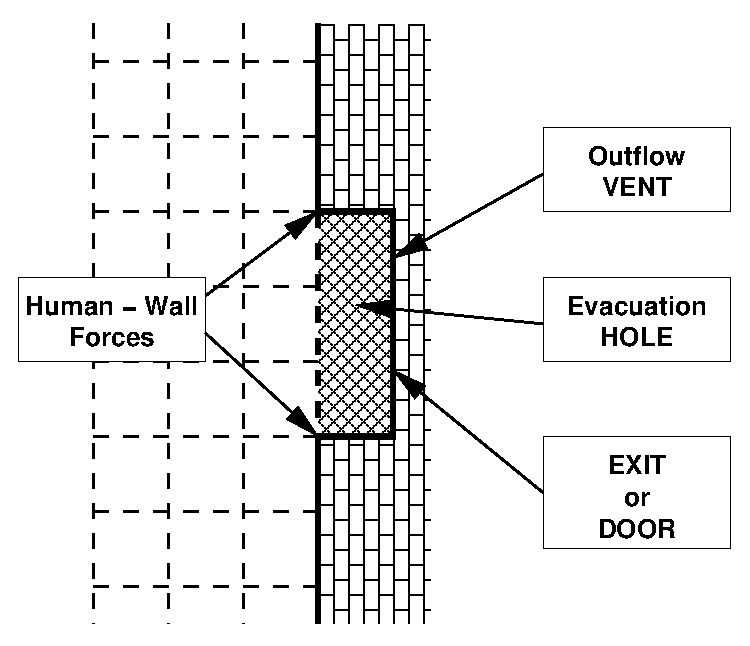
\includegraphics[clip=true,
    width=80mm]{door_geometry2.eps}}
  \caption{How to make an exit or a door.}\label{Fig_DoorGeom} 
\end{figure}
%

For now, FDS+Evac has limitations on the number of humans, which can
be in the same main evacuation mesh.  The program stops and writes out
an error message if more than 10000 humans are tried to put on the
same evacuation mesh.  Usually, one main evacuation mesh extends over
a whole floor of the building.  There may be many main evacuation
meshes, \emph{e.g.}, different floors of the building, in the FDS+Evac
calculation and the total number of humans is not restricted by the
program, the only limit is the available computer memory.  The user
should know that if there is more than a couple of thousands humans on
an evacuation floor then the calculation is going to be CPU expensive.

FDS+Evac enables coupled fire and evacuation simulations.  The
evacuation part uses smoke and gas consentrations from the fire
calculation to affect the movement and decision making of the
evacuating humans.  In principle, the coupling could be made also to
the other direction, \emph{i.e.}, humans are influencing the fire
calculation, \emph{e.g.}, by opening doors, but this feature is not
yet implemented in FDS+Evac.  Concentrations of $\mathrm{O_2}$,
$\mathrm{CO_2}$, and $\mathrm{CO}$ are used to calculate Purser's
Fractional Effective Dose (FED) concept~\cite{Purser95}, which is used
to incapasitate humans.  Smoke density is used both to slow down the
walking speeds of humans and to affect the exit selection algorithm of
humans.  Smoke density can also be used to detect the fire, but is
should be kept in mind that human nose is a very delicate instrument
and the levels of smoke consentration needed for a sensation of smoke
are well below the prediction capabilities of the current FDS fire
model.

The evacuation part of the FDS+Evac is stochastic, \emph{i.e.}, it
uses random numbers to generate the initial positions and properties
of humans and there are also a small random force on each human's
equation of motion.  Thus, same results are not obtained for a given
input file if multiple simulations are done.  For this reason, one
should always do a dozen or so egress simulation to see the variation
of the results.  Because of this, it is made posible to do many egress
calculation per one fire simulation and the calculation of the
evacuation flow fields used to guide human movement need to be
calculated only once to each given geometry, which will speed up the
computation.

The present version of FDS+Evac does not use optimally computer memory
and does not support parallel CPU calculations.  In later versions of
the program, the memory usage is more optimal and also the fire
simulation part can be run using parallel CPUs to produce smoke and
gas concentration informtion for the evacuation part.



\subsection{Intended User's of FDS+Evac}\label{Sec_IntUsers}

FDS+Evac is primarly a research tool for studying evacuation processes
in buildings.  While it seems to produce similar egress flows as found
in the litterature (both experimental and other simulation tools) it
is not yet fully validated.  Thus, its use as an engineering tool
needs further considerations.  It is suggested that FDS+Evac is used
together with some other (well) validated egress program to study
evacuation.  If the two (or more) methods give similar results then
the predictions of the calculational modelling should be quite good.
For example, one could compare the calculations done with ``fire
drill'' mode and used FDS+Evac to study the effects of smoke and toxic
gases on the evacuation, if the other evacuation programme does not
support importing the fire related data from FDS calculations.  Note
that the underlaying assumptions on the fire and evacuation scenarios
might still be far off. It is not the purpose of this document (nor
FDS+Evac) to give instructions on how to define good scenarios and
input data for egress simulations to be done when designing a safe
building.  Fire regulators and designers should agreee on the relevant
scenarios before any design by the engineering methods.


\clearpage

\section{Model Documentation}\label{Sec_ModelDef}

This section provides a short description of the evacuation module of
the Fire Dynamics Simulator (FDS).  Detailed information about FDS can
be found in its documentation and more detailed information about the
evacuation algorithm and its features can be found in the next
chapters.



\subsection{Name and Version of the Model}

The name of the underlaying fire simulation program is the NIST Fire
Dynamics Simulator or FDS.  FDS is a Fortran 90 computer program that
solves the governing equations of fluid dynamics, and Smokeview is a
companion program written in C/OpenGL programming language that
produces images and animations of the results.  The evacuation
calculation module developed at VTT is implemented as subroutines of
FDS and these subroutines together with the FDS are called as the
FDS+Evac.  Since the version 5 of FDS, the program development and
maintenance has utilized a version cotrol system (SVN).  The source
code is maintained at a public domain server.\footnote{The server is
  hosted by Google Code (http://code.google.com/p/fds-smv/)} The
present version of FDS+Evac is build on the FDS version 5.1.2 and it
is the second version of the evacuation module and, thus, its version
number is 2.0.0, \emph{i.e.}, FDS5.1.2+Evac2.0.0.  Changes in the
version numbers correspond to major changes in the physical models or
input parameters.  For minor changes and bug fixes, incremental
versions are released, referenced according to fractions of the
integer version numbers.  In addition, day-to-day bug fixes made in
response to user feedback are referenced by a compilation date and a
SVN revision number that are printed at the top of the diagnostic
output file.  The latest official release version of FDS is obtainable
on the web site http://fire.nist.gov/fds/.  The most recent version of
the evacuation part and the documentation on the evacuation part of
FDS+Evac can be found on the page http://www.vtt.fi/fdsevac/.

\subsection{Type of the Model}

FDS+Evac is a combined agent-based egress calculation model and a
Computational Fluid Dynamics (CFD) model of fire-driven fluid flow,
where the fire and egress parts are interacting.  FDS+Evac can also be
used just to calculate the egress problem without any fire-driven
fluid flow calculation, \emph{e.g.}, it can be used to simulate fire
drills.  FDS+Evac models the egress of humans using continuous space
and time.

\subsection{Model Developers}

The evacuation module of FDS was developed and its currently
maintained by the VTT Technical Research Centre of Finland (VTT).  A
substantial contribution to the implementation of the evacuation
calculation as a module of FDS was made by the Fire Research Division
in the Building and Fire Research Laboratory at the National Institute
of Standards adn Technology (NIST).  Additional contributors and
co-workers are cited in the Acknowledgments.

\subsection{Relevant Publications}

Each version of FDS+Evac is documented by this publication -- the
FDS+Evac Technical Reference and User's Guide.  The User's Guide part
of the publication explains the mechanics of using the computer
programme.  The Technical Reference Guide part provides the theory and
the details of the algorithms, plus a description of the verification
and validation studies and details about the many parameters of the
evacuation model and their default values.  This section contains also
a throughout study of the effects of the model parameters on the
calculated egress flows.

The model behind the movement algorithm of FDS+Evac was introduced by
Helbing \emph{et al.}~\cite{Helbing95,Helbing00,Helbing02,Werner03}.
The implementation of this algorithm inside the FDS program
environment was introduced by Korhonen \emph{et
  al.}~\cite{Korhonen05}.  Later the model was modified along the
lines given in the paper by Langston \emph{et al.}~\cite{Langston06}
to a three circle representation of humans by Korhonen \emph{et
  al.}~\cite{Korhonen07a}.

\subsection{Input Data Required to Run the Model}

All of the input parameters required by the evacuation part of
FDS+Evac to describe a particular scenario are conveyed via one text
file, which is the same one that is used for FDS, created by the user.
For the fire-driven fluid flow related parameters, see the FDS
documentation~\cite{FDS_UserGuide}.  The input file of FDS+Evac is
such that it can be used with just a minor modifications to run an
ordinary FDS calculation without evacuation calculation.  These minor
modifications means that only the definitions of the evacuation meshes
should be commented out, \emph{i.e.}, all the other evacuation related
parameters are neglected by the FDS fire calculation.

A complete description of the input parameters required by the
evacuation module of FDS can be found in the User's Guide part of this
document.

\subsection{Model Results}

FDS+Evac computes the position, the velocity, and the dose of toxic
gases of each agent inside the computational domain at each discrete
time step.  The movement of agents can be visualized after simulation
using the Smokeview program~\cite{SV_UserGuide}.  The number of agents
gone through different parts of the evacuation scenario as well as the
number of agents in different nodes are saved in simple,
comma-delimeted text file, that can be plotted using a spreadsheet
program.  Some additional, quite detailed, information are written to
the diagnostic standard error channel, which could be redirected to
the hard disk for later use.

\subsection{Uses and Limitations}\label{Sec_UsesAndLimit}

Although FDS+Evac can address many egress scenarios, there are
limitations in all of its algorithms.  Some of the more prominent
limitations of the model are listed here.

\underline{Geometry:} The efficiency of FDS is due to the simplicity
of its rectilinear numerical mesh.  This can be a limitation in some
situations where certain geometric features do not conform to the
rectangular mesh.  The numerical meshes used by the human movement
algorithm of FDS+Evac are two-dimensional cut-offs of the FDS fire
meshes, thus the same limitations apply to the evacuation part of the
code.  The present version of the evacuation module can also treat
inclines, like wide stairs and spectator stands, which are along the
$x$ or $y$ direction of the underlaying rectangular mesh.  The grid
cell size determines the finest details which can be modelled by the
program and the geometry of the building is discretized, \emph{e.g.},
the widths of the doors are integral multiples of the grid cell sizes.

\underline{Reduced Visibility:} The smoke consentration calculated by
the FDS is used to slow down human movement using the results of a
recent experiment by Frantzich and Nilsson~\cite{Frantzich03}, where
larger smoke consentration were used than in the experiments by
Jin~\cite{Jin78}.  There are large scatter in the experimental results
and more experimental results are more than welcome.  The default
model for stairs does not include the option for humans to turn back
when the smoke consentration becomes too high.

\underline{Incapacitation:} The incapacitation model is the FED
consept introduced by Purser~\cite{Purser95}, but the large scatter
between different humans is not taken into account in the current
version of the program.  Whereas FDS is doing well for the smoke
transport and the prediction of O${}_2$ levels, it does much worse on
the prediction of the CO concentration.  In the standard mixture
fraction model of FDS, the amount of CO produced is decided by the
user input.  Note, that the effect of HCN is not modelled.

\underline{Exit Route Selection:} The exit door selection algorithm is
still a relatively simple one.  It does not include any kind of social
interactions, like herding behavior.  The user has also more or less
full control on the doors which different human groups will be using.
In some applications this can be listed as a benefit of the model, but
this leaves too much trust on the user's expertise and/or intentions.

\underline{Detection and Reaction Times:} The pre-movement time of the
evacuating humans is decided by the user input by giving distributions
for the detection and reaction times.  In addition to the detection
time given user input, the local smoke consentration can be used to
trigger the detection of a fire.

\underline{Applications:} There is no model for elevators in the
current version of the FDS+Evac.  Nor there is any specific objects
relevant to maritime applications.  Concert halls and sport facilities
may be difficult to model due to the limitations dictated by the
rectangular computational mesh.  There is limitation on the number of
humans per evacuation mesh (usually one mesh per one floor).  In the
present version one floor can contain at most 10000 humans.

\clearpage


\section{Theoretical Basis for the Evacuation Model}\label{Sec_BasisModel}

\subsection{Introduction}


FDS+Evac follows each person by an equation of motion.  This approach
allows each person to have his/her own personal properties and escape
strategies, \emph{i.e.}, persons are treated as autonomous agents.
FDS+Evac allows the modelling of high crowd density situations and the
interaction between evacuation simulations and fire simulations.  Some
social interactions among the agents are introduced in the model.  A
reaction function model is used to select the exit routes.  The size
of each agent is represented by three circles approximating the shape
of the human body.  Agents experience contact forces and moments as
well as psychological and motive forces and moments.  The resulting
equations of motions for the translational and rotational degrees of
freedom are solved using the methods of dissipative particle dynamics
on 2D planes representing the floors of a building.  Thus, the model
uses continuous time and space to track the trajectories of the
agents.

The existing fire simulation environment of FDS is used to minimise
the programming effort to write an egress programme.  For
visualisation, the existing Smokeview programme\cite{SV_UserGuide}
developed at NIST is used.  Additional benefit of using FDS as the
platform of an egress model is the direct and easy access to the fire
related properties, like gas temperatures, smoke and gas densities,
and radiation levels at each point in the computational grid.  These
quantities can be used to model the behaviour of evacuating humans.


%
\begin{figure}[!bt]
  \centerline{\includegraphics[ clip=true, width=100mm
  ]{body_shape_forces.eps} } 
\caption{Definitions of the human dimensions and the radial vectors $
  \mathbf{R}^c$ and $\mathbf{R}^{soc}$. }\label{Fig_BodySize}
\end{figure}
%


\subsection{Human Movement Model}\label{Sec_MoveModel}

The method of Helbing's group is used as the starting point of the
human movement algorithm of FDS+Evac.  This model is shortly described
below.  For a longer description, see the papers by Helbing's
group~\cite{Helbing95, Helbing00, Helbing02, Werner03} and references
therein.  For the modification of the one-circle representation of a
human to a three-circle one, see the papers by Langston {\em et
  al.}~\cite{Langston06} and Korhonen {\em et al.}~\cite{Korhonen07a}

FDS+Evac uses the laws of mechanics to follow the trajectories of the
agents during the calculation.  Each agent follows its own equation of
motion:\newline
%
\begin{equation}\label{Eq_motion}
   m_i \frac{d^2 \mathbf{x}_i (t)}{dt^2} = \mathbf{f}_i (t)  +
  {\boldsymbol  \xi}_i (t) ~,  
\end{equation}
%
where $\mathbf{x}_i (t)$ is the position of the agent $i$ at time $t$,
$\mathbf{f}_i (t)$ is the force exerted on the agent by the
surroundings, $m_i$ is the mass, and the last term, ${\boldsymbol
  \xi}_i (t)$, is a small random fluctuation force.  The velocity of
the agent, $\mathbf{v}_i (t)$, is given by $d\mathbf{x}_i/dt$.
FDS+Evac treats humans as combination of three elastic circles moving
on a two-dimensional plane~\cite{Langston06}.  These circles are
approximating the elliptical shape of the human body similarly as in
the Simulex model~\cite{Simulex96} and in the MASSEgress
model~\cite{Pan06}, see Fig.~\ref{Fig_BodySize}.  The default body
dimensions and the unimpeded walking speeds of different predefined
human types of FDS+Evac are listed in Table~\ref{Table_DefaultHumans}.

The force on the agent $i$ has many components:\newline
%
\begin{equation}\label{Eq_force}
  \mathbf{f}_i = \frac{m_i}{\tau_i} \left( \mathbf{v}_i^0 -
    \mathbf{v}_i\right) + \sum_{j \ne i} \left( \mathbf{f}_{ij}^{soc}
    + \mathbf{f}_{ij}^{att} + \mathbf{f}_{ij}^{c} \right) + \sum_{w}
  \left( \mathbf{f}^{soc}_{iw} + \mathbf{f}^{c}_{iw} \right) + \sum_{k}
  \mathbf{f}_{ik}^{att} ~,
\end{equation}
%
where the first sum describes agent--agent interactions, the sum over
$w$ describes agent--wall interactions, and the last term,
$\mathbf{f}_{ik}^{att}$, may be used for other agent--environment
interactions, like the fire--human repulsion.  The first term on the
right hand side describes the motive force on the evacuating human.
Each agent tries to walk with its own specific walking speed, $v^0_i =
\vert \mathbf{v}_i^0 \vert$, towards an exit or some other target,
whose direction is given by the direction of the field $
\mathbf{v}_i^0 $.  The relaxation time parameter $\tau_i$ sets the
strength of the motive force, which makes an agent to accelerate
towards the preferred walking speed.

The agent--agent interaction force in Eq.~\ref{Eq_force} has three
parts.  For the social force term, $\mathbf{f}_{ij}^{soc}$, the
anisotropic formula proposed by Helbing {\em et al.}~\cite{Helbing02}
is used\newline
%
\begin{equation}\label{Eq_socialforce}
 \mathbf{f}_{ij}^{soc} = A_i e^{-(r_{ij}-d_{ij})/B_i }
 \left ( \lambda_i + (1-\lambda_i) \frac{1 + \cos \varphi_{ij}}{2}
 \right )  \mathbf{n}_{ij} ~, 
\end{equation}
%
where $r_{ij}$ is the distance between the centres of the circles
describing the agnets, $d_{ij}$ is the sum of the radii of the
circles, and the vector $\mathbf{n}_{ij}$ is the unit vector pointing
from agnet $j$ to $i$.  For a three circle representation of humans,
the circles used in Eq.~\ref{Eq_socialforce} are those circles of the
two agents, which are closest to each other.  The angle $\varphi_{ij}$
is the angle between the direction of the motion of the agent $i$
feeling the force and the direction to the agent $j$, which is
exerting the repulsive force on the agent $i$.  The parameters $A_i$,
$B_i$ describe the strength and spatial extent of the force,
respectively. The parameter $\lambda_i$ controls the anisotropy of the
social force. If $\lambda_i=1$, then the force is symmetric and if it
is $ 0 < \lambda_i <1$, the force is larger in front of an agent than
behind.  The parameters $A_i$, $B_i$, and $\lambda_i$ could be
different for each agent but in the present version of FDS+Evac they
have same values for each agent.  The psychological wall--agent
interaction, $ \mathbf{f}_{ij}^{soc}$, is treated similarly, but
values $A_w$, $B_w$, and $\lambda_w$ are used for the force constants.
The physical contact force between agents, $\mathbf{f}_{ij}^{c}$, is
given by\newline
%
\begin{equation}\label{Eq_contactforce}
  \mathbf{f}_{ij}^{c} = \left( k (d_{ij}-r_{ij}) + c_d \Delta
    v_{ij}^{n} \right) \mathbf{n}_{ij} + \kappa (d_{ij}-r_{ij})\Delta
  v_{ij}^{t} \, \mathbf{t}_{ij} ~,
\end{equation}
%
where $\Delta v_{ij}^{t}$ is the difference of the tangential
velocities of the circles in contact, $\Delta v_{ij}^{n}$ is the
difference of their normal velocities, and vector $\mathbf{t}_{ij}$ is
the unit tangential vector of the contacting circles.  This force
applies only when the circles are in contact, \emph{i.e.},
$d_{ij}-r_{ij} \ge 0$.  The radial elastic force strength is given by
the force constant $k$ and the strength of the frictional force by the
force constant $\kappa$.  Note, that Eq.~\ref{Eq_contactforce}
contains also a physical damping force~\cite{Langston06} with a
damping parameter $c_d$, which the original model by Helbing {\em et
  al.} does not have.  This parameter reflects the fact that the
collision of two humans is not an elastic one.  The physical
wall--agent interaction, $ \mathbf{f}^{c}_{iw}$, is treated similarly
and same force constants are used.  The term $\mathbf{f}_{ij}^{att}$
can be used to describe attraction (or repulsion) between humans, like
a herding behaviour or an adult--children interaction.  It could also
be used to form pairs of humans, e.g., describing a fire fighter pair
entering the building.  All of the force terms in Eq.~\ref{Eq_force}
are relatively short ranged and they need a line-of-sight connection.
Longer ranged forces could be taken in to account by changing the
preferred walking velocity field $ \mathbf{v}_i^0 $.

Equations~\ref{Eq_motion}--\ref{Eq_contactforce} describe the
translational degrees of freedom of the evacuating agents.  The
rotational degrees of freedom are treated similarly, \emph{i.e.}, each
agent has its own rotational equation of motion:
%
\begin{equation}\label{Eq_rotmotion}
   I^z_{i} \frac{d^2 \varphi_i (t)}{dt^2} = {M}^z_{i} (t)  +
  {\eta}^z_{i} (t) ~,  
\end{equation}
%
where $\varphi_i(t)$ is the angle of the agent $i$ at time $t$,
$I^z_{i}$ is the moment of inertia, ${\eta}^z_{i} (t)$, is a small
random fluctuation torque and ${M}^z_{i} (t)$ is the total torque
exerted on the agent by its surroundings
%
\begin{equation}\label{Eq_total_torque}
  {M}^z_{i} =  {M}^c_{i} + {M}^{soc}_{i} +  {M}^{\tau}_{i} ~,
\end{equation}
%
where ${M}^c_{i}$, ${M}^{soc}_{i}$, and ${M}^{\tau}_{i}$ are the
torques of the contact, social and motive forces, respectively.

The torque of the contact forces is calculated as
%
\begin{equation}\label{Eq_fc_torque}
  \mathbf{M}^c_{i} = \sum_{j \ne i} \left( \mathbf{R}^c_{i} \times
  \mathbf{f}_{ij}^{c} \right) ~, 
\end{equation}
%
where $\mathbf{R}^c_{i}$ is the radial vector which points from the
centre of the agent $i$ to the point of contact.  In FDS+Evac, also
the social forces exert torques on agents and these are given by the
formula
%
\begin{equation}\label{Eq_soc_torque}
  \mathbf{M}^{soc}_{i} =  \sum_{j \ne i} \left( \mathbf{R}^{soc}_{i}
  \times \mathbf{f}_{ij}^{soc} \right) ~,
\end{equation}
%
where only the circles, which are closest to each other, are
considered.  The vector $\mathbf{R}^{soc}_{i}$ points from the centre
of the agent $i$ to the fictitious contact point of the social force,
see Fig.~\ref{Fig_BodySize}.

Analogous to the motive force, the first term on the right hand
side of Eq.~\ref{Eq_force}, a motive torque is defined as
%
\begin{equation}\label{Eq_motive_torque}
  {M}^{\tau}_{i} = \frac{ I^z_{i} }{ \tau^z_{i} } \left( (\varphi_i(t)
    - \varphi^0_{i} ) \omega^0_i - \omega(t) \right) = \frac{ I^z_{i}
  }{ \tau^z_{i} } \left( \tilde \omega^0_i - \omega(t) \right) ~,
\end{equation}
%
where $\omega^0_i $ is the maximum target angular speed of a turning
agent, $\omega (t)$ the current angular velocity, $\varphi_i(t)$ the
current body angle, and $\varphi^0_{i}$ is the target angle,
\emph{i.e.}, where the vector $ \mathbf{v}_i^0 $ is pointing.  The
target angular speed, $\tilde \omega^0_i$, defined in
Eq.~\ref{Eq_motive_torque} is larger when the body angle differs much
from the desired movement direction.  Langston {\em et
  al.}~\cite{Langston06} used a different formula for the motive
torque, which had a form of a spring force.  During this work, it was
noticed that a force like that will make agents to rotate around their
axis like harmonic oscillators and, thus, some angular velocity
dependent torque should be used.

In FDS+Evac method, agents are guided to exit doors by the preferred
walking direction vector field, $ \mathbf{v}_i^0$, and this field is
obtained using the flow solver of the FDS.  This vector field is
obtained as an approximate solution to a potential flow problem of a
two-dimensional incompressible fluid to the given boundary conditions,
where all walls are inert and the chosen exit door acts as a fan,
which extracts fluid out of the domain.  This method, or rather a
trick, produces a nice directional field for egress towards the chosen
exit door, see Fig.~\ref{Fig_EvacFlowField}.  A field of this kind
will always guide agents to the chosen exit door.  This route will not
be the shortest one, but usually it is quite close to it.  This field
will guide more agents to the wider escape routes than on the narrower
ones due to the fact that the field is a solution to an incompressible
flow.  Note, that in the present version of FDS+Evac, escaping agents
have a rule for the exit door selection.  Thus, the above sentence
applies when there are many routes to the chosen exit door or when the
user is allowing more than one exit door per a flow field.  The
analogy to an incompressible fluid flow is not a bad starting point to
find the movement directions of large human crowds.  For example, when
humans are leaving a large sports or entertainment event, they usually
just follow the human flow to the outside of the building without much
control on the process.

%
\begin{figure}[!tb]
  \centerline{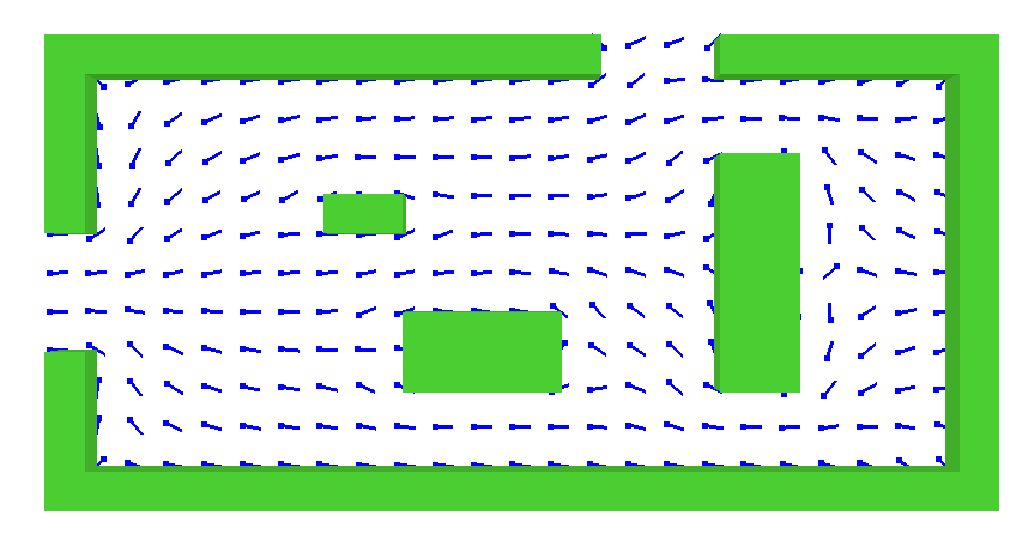
\includegraphics[clip=true,width=120mm]{evac_ffield.eps}}
  \caption{A 2D flow field used to guide humans to the exit doors.  In
    this case, only the left exit has an ``outflow'' boundary
    condition, \emph{i.e.}, this fictitious human flow field is used
    to find the left exit only.  The main evacuation mesh should also
    have an ``outflow'' boundary at the top
    exit.}\label{Fig_EvacFlowField}
\end{figure}
%

The human movement method presented in
Eqs.~\ref{Eq_motion}--\ref{Eq_motive_torque} has many parameters.
Some of these parameters are related to physical dimensions of humans,
like $m_i$ and $I^z_{i}$, but many parameters are related to the
chosen model.  Some of these parameters are chosen to be the same as
found in the literature~\cite{Helbing00,Langston06} and some are
estimated from test calculations.  The parameters of the social force
were chosen such that the specific human flows through doors and
corridors were appropriate.  The parameters for the three circle
representation of the contact forces and the rotational degrees of
freedom were selected mainly by trial and error in order to obtain
reasonably realistic human movement.  Monte Carlo simulations were
done to see, which are the most important model parameters and further
analysis was focused on those parameters.

The first choice for the social force parameters of agent--agent
interaction was $A_i = 2000~\textrm{N}$, $B_i = 0.04~\text{m}$, and
$\lambda_i = 0.5$.  For the agent--wall interaction values $A_w =
2000~\textrm{N}$, $B_w = 0.08~\textrm{m}$, and $\lambda_w = 0.2$ were
used.  It was noticed that these values are not good for congested
situations when three circles are used to describe a human body.
These parameters were modified such that the interaction strength
parameter $A$ was made velocity dependent, $A(v_i) = 2000\,
\mathrm{Max}(0.5, v_i/v^0_i)~\textrm{N}$.

For the contact force parameters, values $k = 12 \times 10^4 ~\mathrm{
  \textrm{kg} \, \textrm{m}^\textrm{-2} }$, $\kappa = 4 \times 10^4
~\mathrm{ \textrm{kg} \, \textrm{s}^\textrm{-1} \textrm{m}^\textrm{-1}
} $, and $c_d = 500 ~\mathrm{\textrm{kg} \, \textrm{s}^\textrm{-1} } $
are used both for the agent--agent and for the agent--wall
interactions.  The mass of a default male agent is $m_i = 80$~kg and
its moment of inertia was chosen to be $I^z_{i} = 4.0 ~\mathrm{
  \textrm{kg} \, \textrm{m}^\textrm{2} }$.  For other agents, the mass
and the moment of inertia are obtained by scaling.  For the angular
relaxation time parameter, $\tau_z$, a value of 0.2~s is used.  The
angular velocity parameter $\omega^0_i$ has a value of $4\pi~\mathrm{
  \textrm{s}^\textrm{-1} } $, \emph{i.e.}, two rounds per second, in
FDS+Evac.  The random force in Eq.~\ref{Eq_motion} is taken to be a
Gaussian with mean zero and standard deviation of $ {\xi}_i/m_i = 0.1
~\mathrm{ \textrm{m} \, \textrm{s}^\textrm{-2}}$.  The random torque
in Eq.~\ref{Eq_rotmotion} is treated similarly and its standard
deviation is $ {\eta}^z_{i}/ I^z_{i} = 0.1 ~\mathrm{
  \textrm{s}^\textrm{-2}}$.

% !Timo: Gaussian random noise
% !Timo: mean, theta (sigma=sqrt(theta)), cut multiplier
% !Timo: 8 Aug 2006: velocity dependent random noise: v > 0.9v0, theta=theta_input
% !Timo: v=0, theta=100*theta_input, 0<v<0.9v0 linear interpolation.
% Edell� force=kiihtyvyys (eli oikea voima = massa*rnd_number)
% Ja torque=rnd_number*M_iner 
%defaults: noiseth=0.01 (eli stddev 0.1), noisecm=3.0*(std.dev)

In principle, all the above parameters may be dependent on the person
in question. But in FDS+Evac, only the body sizes, walking velocities,
and the motive force parameter $\tau_i$ are personalised by choosing
them from a random distribution. A uniform distribution ranging from
0.8~s to 1.2~s is used for $\tau_i$ and the used uniform distributions
for the body dimensions and for the walking speeds are shown in
Table~\ref{Table_DefaultHumans}.



\subsection{Fire and Human Interaction}\label{Sec_FireHumanInt}

By using FDS as the platform of the evacuation calculation we have
direct and easy access to all local fire related properties, like gas
temperature, smoke and gas densities, and radiation levels.  Fire
influences evacuation conditions; it may incapacitate humans and in
extreme cases block major exit routes.  On the other hand, humans may
influence the fire by opening doors or actuating various fire
protection devices.  For now, the effect of smoke on the movement
speeds of agents and the toxic influence of the smoke are implemented
in movement algorithm of FDS+Evac.  The exit selection algorithm of
the agents uses smoke density to calculate the visibility of the exit
doors and to categorize the doors to different preference groups.

Smoke reduces the walking speed of humans due to the reduced
visibility, its irritating and asphyxiant effects.  Recently,
Frantzich and Nilsson~\cite{Frantzich03} made experiments on the
effect of smoke concentration on the walking speeds of humans.  They
used larger smoke concentrations than Jin~\cite{Jin78} and they fitted
the following formula to the experimental values
%
\begin{equation}\label{Eq_SpeedSmoke}
  v^0_i (K_s) = \frac{v^0_i}{\alpha} ( \alpha + \beta K_s ) ~,
\end{equation}
%
where $K_s$ is the extinction coefficient ($[K_s] \!\! = \!\!
\mathrm{ \textrm{m}^\textrm{-1} } $) and the values of the
coefficients $\alpha$ and $\beta$ are 0.706~$\mathrm{ \textrm{m} \,
  \textrm{s}^\textrm{-1} } $ and -0.057~$\mathrm{
  \textrm{m}^\textrm{2} \textrm{s}^\textrm{-1} } $, respectively.  The
standard deviations are reported to be $\sigma_\alpha = 0.069~\mathrm{
  \textrm{m} \, \textrm{s}^\textrm{-1} } $ and $\sigma_\beta = 0.015~
\mathrm{ \textrm{m}^\textrm{2} \textrm{s}^\textrm{-1} } $, but only
the mean values are used in FDS+Evac, \emph{i.e.}, there is no variation
between the agents.

The toxic effects of gaseous fire products are treated by using
Purser's Fractional Effective Dose (FED) concept~\cite{Purser95}.  The
present version of FDS+Evac uses only the concentrations of the
narcotic gases CO, CO${}_2$, and O${}_2$ to calculate the FED value
%
\begin{equation}
\mathrm{FED}_\mathrm{tot} = \mathrm{FED}_\mathrm{CO} \times
\mathrm{HV}_\mathrm{CO_2} + \mathrm{FED}_\mathrm{O_2} 
\end{equation}
%
Note, that the above equation does not contain the effect of HCN,
which is also narcotic, and the effect of CO${}_2$ is only due to the
hyperventilation, \emph{i.e.}, it is assumed that the CO${}_2$ is such
low that it does not have narcotic effects.  Carbon dioxide does not
have toxic effects at consentrations of up to 5 percent but it
stimulates breathing which increases the rate at which the other fire
products are taken up.  The fraction of an incapacitating dose of CO
is calculated as
%
\begin{equation}
\mathrm{FED}_\mathrm{CO} = 4.607 \cdot 10^{-7} (C_\mathrm{CO})^{1.036}
\ t ~,
\end{equation}
%
where $t$ is time in seconds and $C_\mathrm{CO}$ is the CO
concentration (ppm).  The fraction of an incapacitating dose of low
O${}_2$ hypoxia is calculated as
%
\begin{equation}
\mathrm{FED}_\mathrm{O_2} =  \frac{t}{60 \exp \left [ 8.13-0.54 (20.9 -
  C_\mathrm{O_2}) \right ] } ~, 
\end{equation}
%
where $t$ is time in seconds and $C_\mathrm{O_2}$ is the O${}_2$
concentration (volume per cent).  The carbondioxide induced
hyperventilation factor is calculated as
%
\begin{equation}
\mathrm{HV}_\mathrm{CO_2} = \frac{ \exp( 0.1930 \, C_\mathrm{CO_2} +
  2.0004 ) }{7.1} ~, 
\end{equation}
%
where $C_\mathrm{CO_2}$ is the CO${}_2$ concentration (percent).

An agent is considered to be incapacitated when the FED value exceeds
unity.  An incapacitated agent is modelled as an agent, which does not
experience any social forces from the other agents and whose target
movement speed, $v^0_i$, is set to zero.  The size of an incapacitated
agent is not changed, \emph{i.e.}, it remains on its feet.  This is a
very crude model and it needs to be modified in later versions of
FDS+Evac.



\subsection{Exit Selection}\label{Sec_ExitSel}

Game theoretic reaction functions and best response dynamics are
applied to model the exit route selection of
evacuees~\cite{Heliovaara07}.  In the model, each evacuee observes the
locations and actions of the other evacuees and selects the exit
through which the evacuation is estimated to be the fastest.  Thus,
the exit selection is modelled as an optimisation problem, where each
evacuee tries to select the exit that minimises the evacuation time.
The estimated evacuation time consists of the estimated time of
walking and the estimated time of queueing.  The walking time is
estimated by dividing the distance to the exit by the walking speed.
The estimated time of queueing is a function of the actions and
locations of the other evacuees.  It is also assumed that people
change their course of action only if there is an alternative that is
clearly better than the current choice.  This behaviour is taken into
account by subtracting a parameter from the estimated evacuation time
of the exit currently chosen.

%
\begin{table}[!tp]
\caption{Preference order used in the exit selection algorithm.  The 
last two rows have no preference.  This is because the evacuees are
unaware of the exits that are unfamiliar and invisible and, thus,
can not select these exits.}\label{Table_pref_order}
\begin{center}
\begin{tabular}{c|c|c|c} \hline \hline
preference&visible&familiar&disturbing conditions\\ \hline 1&yes&yes&no\\
\hline
2&no&yes&no\\ \hline 3&yes&no&no\\ \hline 4&yes&yes&yes\\ \hline 5&no&yes&yes\\
\hline 6&yes&no&yes\\ \hline No preference&no&no&no\\
\hline No preference&no&no&yes\\ \hline \hline
\end{tabular}
\end{center}
\end{table}
%

Apart from the locations of exits and the actions of other people,
there are also other factors that influence the evacuees' decision
making.  These factors are the conditions related to the fire, the
evacuees' familiarity with the exits and the visibility of the exits.
The effect of these factors is taken into account by adding
constraints to the evacuation time minimisation problem.  According to
the three factors mentioned, the exits are divided to seven groups so
that each exits will belong to one group.  The groups are given an
order of preference.  
%In the model, the following \emph{preference
%  order} of exit groups is assumed for each evacuee:

The familiarity of each exit for each agent can be determined by the
user in the input-file of FDS+Evac.  It is also possible to give a
probability for the familiarity of an exit, and FDS+Evac will randomly
set the familiarity of the exit.  FDS+Evac determines the visibility
of an exit to an agent by taking into account the blocking effect of
smoke and obstacles.  The possible blocking effect of other agents is
not considered in the current version of the programme.  The existence
of disturbing conditions is estimated from the fire-related data of
FDS on the visible part of the route to the exit.  By disturbing
conditions we mean conditions, like temperature and smoke, that
disturb an evacuee but are not lethal.  If there are lethal conditions
on an exit route, the exit has no preference.

The exit selection algorithm consists of the above described two
phases.  First the exits are divided to the preference groups
according to Table~\ref{Table_pref_order}.  Then, an exit is selected from
the most preferred nonempty preference group by minimising the
estimated evacuation time.

According to socio-psychological literature~\cite{Pan06,Proulx1993},
the familiarity of exit routes is an essential factor influencing
decision making.  This is because the unknown factors related to
unknown routes are considered to increase the threat.  As a result,
evacuees prefer familiar exit routes even if there are faster
unfamiliar routes available.  For this reason, emergency exits are used
rarely in evacuations and fire drills.


\subsection{Groups}\label{Sec_Groups}

According to socio-psychological literature, a crowd consists of small
groups, like families, that tend to act together~\cite{Pan06,
  Matikainen07}.  This behaviour should be taken into account when
building evacuation models.  A method for modelling this grouping
behaviour with the equations of Helbing was
developed~\cite{Heliovaara07}.  In the model, the actions of a
group are divided into two stages:
\begin{enumerate}
\item In the gathering stage the group members walk towards
each other to gather the group.
\item In the egress stage the group moves together along the
selected exit route.% \\[-1.5em]
\end{enumerate}

%
These two stages are modelled by altering the preferred walking
direction field of Helbing's equation of motion.  In the gathering
stage the pedestrians are trying to move towards the centre of the
group.  When the distances from the centre to each pedestrian are
under a threshold value, the group is considered to be complete.  When
a group is complete, it starts to move towards an exit.  This means
that each group member is set to follow the same flow field.  While
moving towards an exit, the group members also try to keep the group
together.  This is modelled by adjusting the walking speeds and by
adding an additional force that points to the centre of the group.
This force is called as the group force.  The magnitude of the group
force describes how eagerly the group members try to keep the group
together.  It can be given different values for different kinds of
groups.  For example, a group consisting of a mother and a child
should have a larger group force than a group of work mates.

The group-model is not yet available in FDS, but it will be added to
later versions of the programme.  The model has been programmed to a
test-version and the results are promising, but quantitative effects
of the model are yet to be analysed.  The results of these analyses
will be presented in a separate paper.


\subsection{Numerical Method}\label{Sec_NumMethod}
%Eli miten eri kohdat on implementoitu.  Eli kuinka useasti tuodaan
%tulipalolaskun datat ihmisille, ihmisten aika-askeleen automaattinen
%s��t�minen, satunnaisvoiman lauseke.  T�nne my�skin se, ett� mitein
%ovet ja k�yt�v�t on mallitettu.  Koodin nopeutus eli blokkimuoto,
%kunhan sen saan implementoitua.

The translational and rotational equations of motion are solved using
a modified velocity-Verlet algorithm, where the translational motive
force part is solved using a self-consistent dissipative
velocity-Verlet algorithm~\cite{Vattulainen02} and the other parts are
solved using the standard velocity-Verlet algorithm, which can be
found in any basic textbooks on molecular dynamics simulations.  The
time step used in the algortihm is adjusted during the simulations by
the maximum forces excerted on humans.  The minimum time step varies
between 0.01 and 0.001 seconds, by default.

The estimated evacuation time used in the exit door selection
algorithm is approximated in the present version of FDS+Evac simply by
dividing the distance to the door by the unimpeded walking velocity of
the person.  The distance to a door is calculated along a bee line
both for the visible and non-visible doors.  The distance should be
calculated along the exit path and also an estimated queueing time at
the door should be added to the estimated evacuation time, but this is
not yet implemented in the model.  Agents are updating their target
exit doors on every second, on the average.

The smoke density calculated by the FDS fire simulation can be used to
detect a fire.  By default, smoke density is not used for detection.
User gives as inputs a detection time (distribution) and a reaction
time (distribution) for the evacuating agents.  If smoke is used to
detect fire then user should give the detection threshold
concentration (mg/m${}^3$).  An agent detects a fire when the smoke
concentration reaches its threshold value at the position of the agent
or if the user given detection time has been reached.

The smoke or toxic gas concentrations affect the exit door selection
algorithm. By default, toxic gas concentrations are used (CO,
CO${}_2$, O${}_2$): a door is 'smoke free' if the estimated value of
FED less than 0.000001.  A door is usable (and visible) as long as the
estimated FED value is less than unity.  If smoke concentration is
used then user gives the threshold visibility value for a door to be
'smoke free'.  A door is usable as long as visibility is larger than
0.5*distance to the door, where visibility = 3/extinction coefficient.
If there is no line-of-sight to the door, then local concentrations at
the position of the agent are used and the distance to the door is
calculated along a bee line (this is a crude approximation but fast to
compute).


\section{Testing and Verification}\label{Sec_TestVerif}

\subsection{Introduction}

In the verification test cases the default parametere values of
FDS+Evac for the different pre-defined human types were used unless
otherwise stated.  In many cases the simulation runs were also done
using a value of 0.3 for the anisotropy parameter of the social force
instead of the default value of 0.5.  An archive of the verification
tests of FDS+Evac are on the FDS+Evac web pages.  This manual contains
only a short summary of these test and it might not be up to date, so
more interested reader should visit the web pages to get the most
recent information.

Note, that the results reported below are just based on one FDS+Evac
simulation per each scenario.  FDS+Evac is a stochastic modelling
program, \emph{i.e.}, it uses stochastic distributions to generate the
initial positions of the agents and their properties.  There are also
small random forces and torques in the equations of motion.  For the
qualitative verification however, it is enough just to run the model
once for each scenario.

Some of the qualitative verification cases of the human movement
algorithm are based on the IMO document ``Interim Guidelines for
Evacuation Analyses for New and Existing Passenger
Ships''~\cite{IMO02}, where eleven different test cases are listed.
These tests are refered below as ``IMO 1'' etc.  Note, that the IMO
document specifies the test persons to be 30--50 years old males
defined in the IMO document~\cite{IMO02}.  This person group is
similar to the default ``Male'' of FDS+Evac but the unimpeded walking
velocities are generated from an uniform distribution between
0.97--1.62~m/s.  If the test case in question is a IMO test case, then
the reference to a ``Male'' default person type is the default
``Male'' of FDS+Evac, but with different walking speed.
%% &PERS ID='Imo1',
%%       FYI='Imo, 30-50 males',
%%       DEFAULT_PROPERTIES='Male',
%%       VELOCITY_DIST=1, VEL_MEAN=1.295,VEL_PARA=0.05,VEL_LOW=0.97,VEL_HIGH=1.62,
%%       PRE_EVAC_DIST=0, PRE_MEAN=0.0,
%%       DET_EVAC_DIST=0, DET_MEAN=0.0,
%%       DENS_INIT = 2.5,
%%       COLOR_METHOD = 7 /

The tests suggested by IMO do not include any quantitative
verification, because IMO sees that ``At this stage of development
there is insufficient reliable experimental data to allow a through
quantitative verification of egress models.  Until such data becomes
available the first three components of the verification process
(component testing, functional verification, qualitative verification)
are considered sufficient.''

\subsection{Component Testing}\label{Sec_CompTest}

The movement algorithm of FDS+Evac was tested first using some simple
geometries to show that the agents do not walk through walls and that
their speed is correct and they move towards the exit doors which the
user has spcified in the input.  These simulations were done in an
evacuation trial mode, \emph{i.e.}, there was no smoke or fire
calculation present in the simulations.  The effect of smoke on the
moving speeds of the humans and the calculation of the FED were tested
separately.


%
\begin{enumerate}
%
\item IMO 1: Maintaining set walking speed in corridor: One person
  with a walking speed of 1.0~m/s should walk a 40~m distance in 40~s.
  FDS+Evac passed the test.
%
\item IMO 2: Maintaining set walking speed up staircase: One person
  with a walking speed of 1.0~m/s should walk a 10~m distance in 10~s.
  FDS+Evac passed the test.  Both existing models for staircases
  (\Timtt{\&CORR} and \Timtt{\&EVSS} namelists in the input) were
  used.
%
\item IMO 3: Maintaining set walking speed down staircase: One person
  with a walking speed of 1.0~m/s should walk a 10~m distance in 10~s.
  FDS+Evac passed the test.  This test is actually the same as the
  test number IMO 2, because the staircase algorithm of FDS+Evac is
  the same for up and down, only the user input for the speed
  reduction factor is changed.
%
\item IMO 4: Exit flow rate: 100 persons in a room with a 1.0~m exit,
  the flow rate should not exceed 1.33~p/s.  FDS+Evac passed the test,
  if an ``Male'' with the parameter value $\lambda_i=0.3$ is used.
  The default for this parameter is 0.5.  See also the door flow test
  case in Sec~\ref{Sec_XX}.  It should be noted that larger specific
  flows through doors than 1.33~p/s/m are obtained if a wider door is
  used.
%
\item IMO 5: Response time: Verify that the humans start to walk
  according to a given uniform reaction time distribution.  FDS+Evac
  passed the test.  FDS+Evac prints out the main personal properties
  of the agents, including their response and detection times,
  unimpeded walking velocities, main body diameters, motive force time
  constants $\tau_i$, and the initial positions.
%
\item IMO 6: Rounding corners: Persons approaching a corner will
  successfully navigate around the corner without penetrating the
  boundaries.  FDS+Evac passed the test.  The social force model used
  for the movement of the agents does not allow the agents to go
  inside walls if the time step is small enough as it is in FDS+Evac
  for reasonable values of the model parameters.
%
\item IMO 7: Assignment of population demographics parameters:
  Distribute the walking speeds over a population of 50 people and
  show that the walking speeds are consistent with the distribution
  specified in the input.  FDS+Evac passed the test, see the test
  number IMO 5 above.
%
\item FED calculation: To test the implementation of Fractional
  Effective Dose (FED) concept~\cite{Purser95} a simple one room
  geometry with a fire source and one agent in the middle of the room
  is used.  The agent is fixed at its initial position by putting the
  detection time large and setting random noise of the movement
  equations to zero.  FDS point measurements of the gas densities are
  placed at the position of the agent.  The FDS+Evac output for the
  value of the maximum FED among the agents is compared to a value
  computed using an external worksheet and the FDS point measurements
  for gas densities.  The results of the comparison are shown in
  Fig.~\ref{Fig_FED_Test}.  The results indicate that the FED
  calculation in FDS+Evac is working correctly.
%
\begin{figure}[!tb]
  \centerline{\includegraphics[clip=true,width=80mm]{FED_Test.eps}}
  \caption{A FED test}\label{Fig_FED_Test}
\end{figure}
%
%
\item Unimpeded walking speed vs smoke density: Smoke reduces the
  walking speed due to the reduced visibility.  The prediction of this
  effect is tested in long corridor geometry.  The source code of
  FDS+Evac was modified a little bit for this test.  The evacuation
  calculation did not use the smoke densities calculated by FDS but an
  artificial smoke density history with stepwise behaviour: soot
  density (extinction coefficient) was increased by
  114.9~mg/$\mathrm{m^3}$ (1.0~$\mathrm{m^\textrm{-1}}$) after every
  10 seconds.  The length of the simulation was 100~s and the
  unimpeded walking velocity for a smokeclear environment was set to
  1.0~m/s.  The result of this test is shown in
  Fig.~\ref{Fig_SmokeSpeedTest}.  In the figure, the line labelled as
  ``Theory'' is the experimental correlation given in
  Eq.~\ref{Eq_SpeedSmoke}.  The velocities were calculated using 8~s
  periods, like 22~s -- 30~s, because an agent needs a little bit time
  to adjust its speed (the inertia of mass) when the smoke density is
  changed.  The results show that FDS+Evac accurately reproduces the
  anticipated reduction of walking speed.
%
\begin{figure}[!tb]
  \centerline{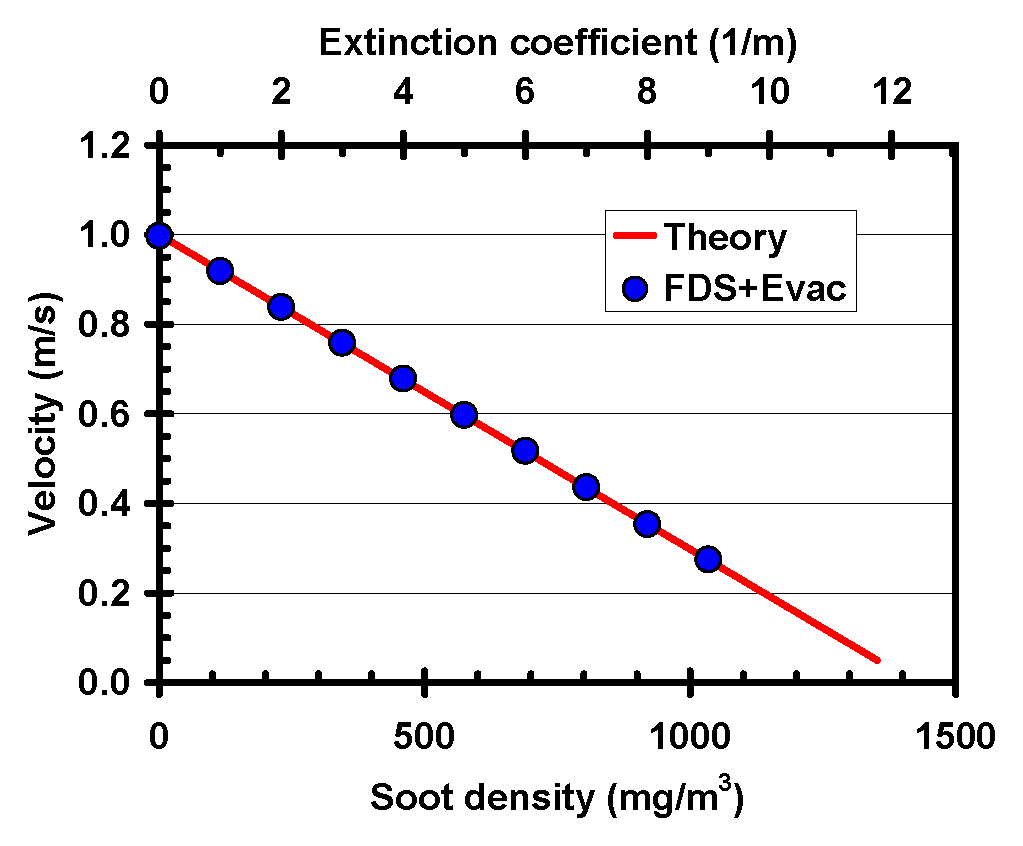
\includegraphics[clip=true,width=80mm]{Smoke_vs_speed.eps}}
  \caption{A smoke vs speed test}\label{Fig_SmokeSpeedTest}
\end{figure}
%
%
\end{enumerate}
%

For the functional verification required by IMO a good technical
documentation should be enough.  The manual should set out in a
comprehensible manner the complete range of model capabilities and
inherent assumptions and give a guide to the correct use of the
capabilities.

\subsection{Qualitative Verification}\label{Sec_QualVeri}


The qualitative features of FDS+Evac were tested using some simple
geometries to show that the agents behave like they are told in the
input and that their movement is qualitatively correct.  Most of these
simulations were done in an evacuation trial mode, \emph{i.e.}, there
was no smoke or fire calculation present in the simulations.  The
effect of smoke and toxic gases on the decision making processes of
the agents were tested separately.

%
\begin{enumerate}
%
\item IMO 8: Counterflow -- two rooms connected via a corridor: Two
  10$\times$10~$\mathrm{m^2}$ rooms are connected with a 10m~long and
  2~m wide corridor.  Initially there are 100 persons in the room 1
  and the room 2 has 0, 10, 50, 100 persons and both rooms move off
  simultaneously.  The expected result is that the time the last
  person from the room 1 enters the room 2 increases as the number of
  persons in counterflow increases.
  
  FDS+Evac results were 43~s and 344~s for the cases, where there were
  0 and 10 persons in the room 2, respectively.  The case, where there
  were 50 persons in the room 2, resulted a very slow movement towards
  the room 2 and the simulation was not run until the end.  If there
  were 100 persons in the room 2 then there were practically no
  movement in the corridor, \emph{i.e.}, a total jam was formed.
%
\item IMO 9: Exit flow -- crowd dissipation from a large public room:
  A 30$\times$20~$\mathrm{m^2}$ public room with four 1.0~m wide exits
  has 1000 persons.  Calculate the time the last person leaves the
  room.  Close two doors and repeat the calculation.  The expected
  result is an approximate doubling of the time to empty the room.
  
  FDS+Evac passed the test.  The total evacuation times calculated
  using the default person properties were 188~s and 354~s when all
  four doors were open and when two doors were closed, respectively.
  These times were 248~s and 470~s when the parameter value
  $\lambda_i$ is changed from the default, which is 0.5, to 0.3.
  Note that the flows through the 1.0~m doors were below 1.33~p/s when
  an ``Male'' with the parameter value $\lambda_i = 0.3$ is used.  The
  default for this parameter is 0.5 and then flows through the doors are
  slightly larger.  See also the door flow test case in
  Sec.~\ref{Sec_XX}.
%
\item IMO 10: Exit route allocation: Populate a cabin corridor section
  with 23 persons and allocate the main exit for 15 persons and the
  secondary exit for 8 persons.  The expected result is that the
  allocated passengers move to the appropriate exits.  FDS+Evac passed
  the test.
%
\item IMO 11: Staircase: A room populated with 150 persons is
  connected to a 2.0~m wide and 12~m long corridor which ends to a
  2.0~ m wide stairs going upwards.  The expected result is that
  congestion appears at the exit from the room, which produces a
  steady flow in the corridor with the formation of congestion at the
  base of the stairs.
  
  FDS+Evac passed the test, if the user is giving reasonable input
  parameters for the definition of the staircase.  Both models for
  staircases \Timtt{\&CORR} and \Timtt{\&EVSS} namelists in the input)
  were used.
%
\begin{figure}[!tb]
  \centerline{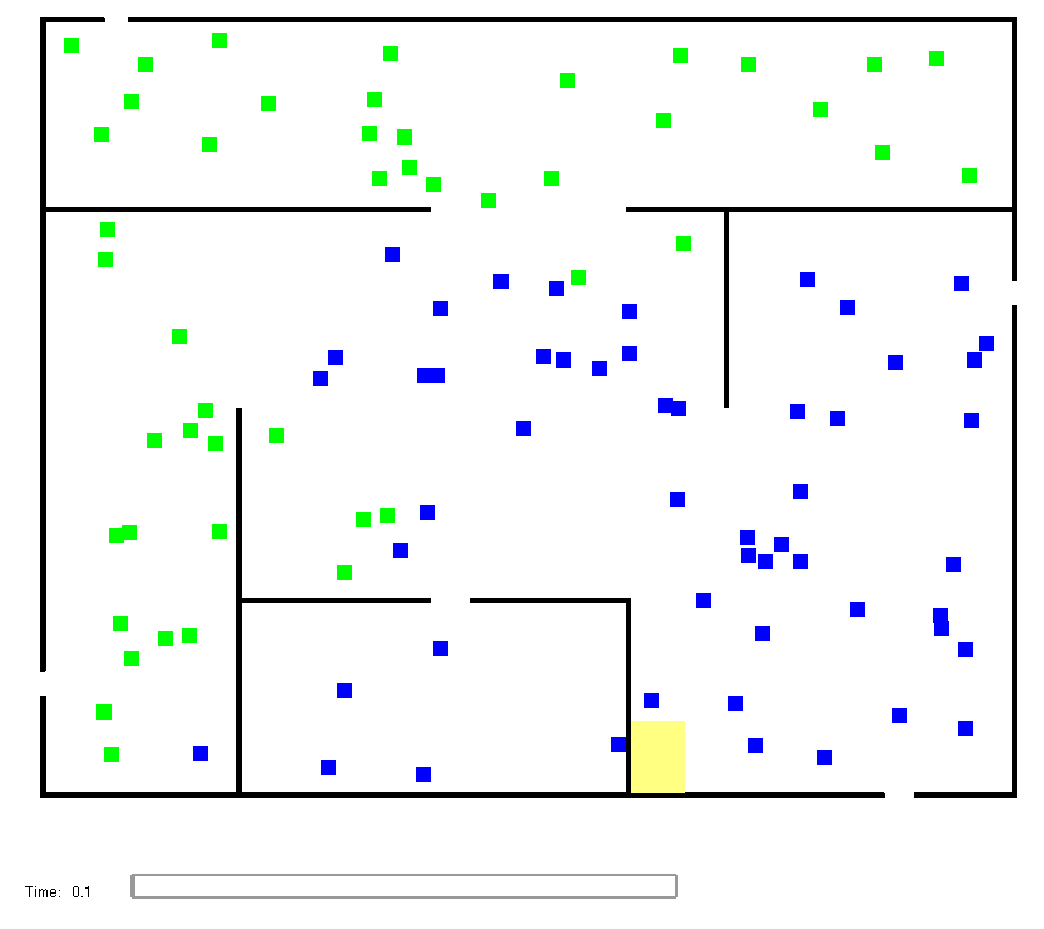
\includegraphics[clip=true,width=60mm]{DoorTestNoSmoke_Doors.eps}
  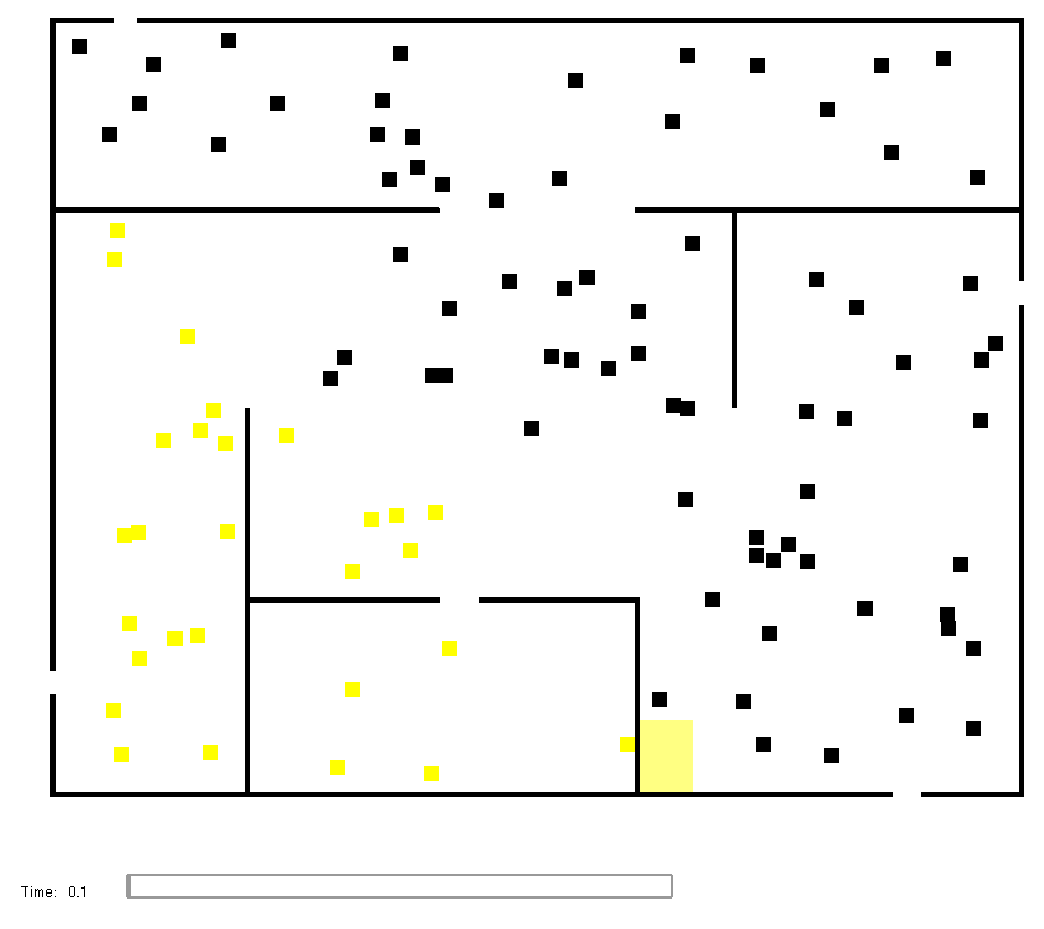
\includegraphics[clip=true,width=60mm]{DoorTestNoSmokeAlgorithm.eps}}
  \caption{An exit door selection test without
    smoke.  On the left, agents are coloured according to their exit
    doors. On the right, they are coloured according to their current
    preference categories.}\label{Fig_ExitDoorNoSmoke}
\end{figure}
%

  
%
\begin{figure}[!bt]
  \centerline{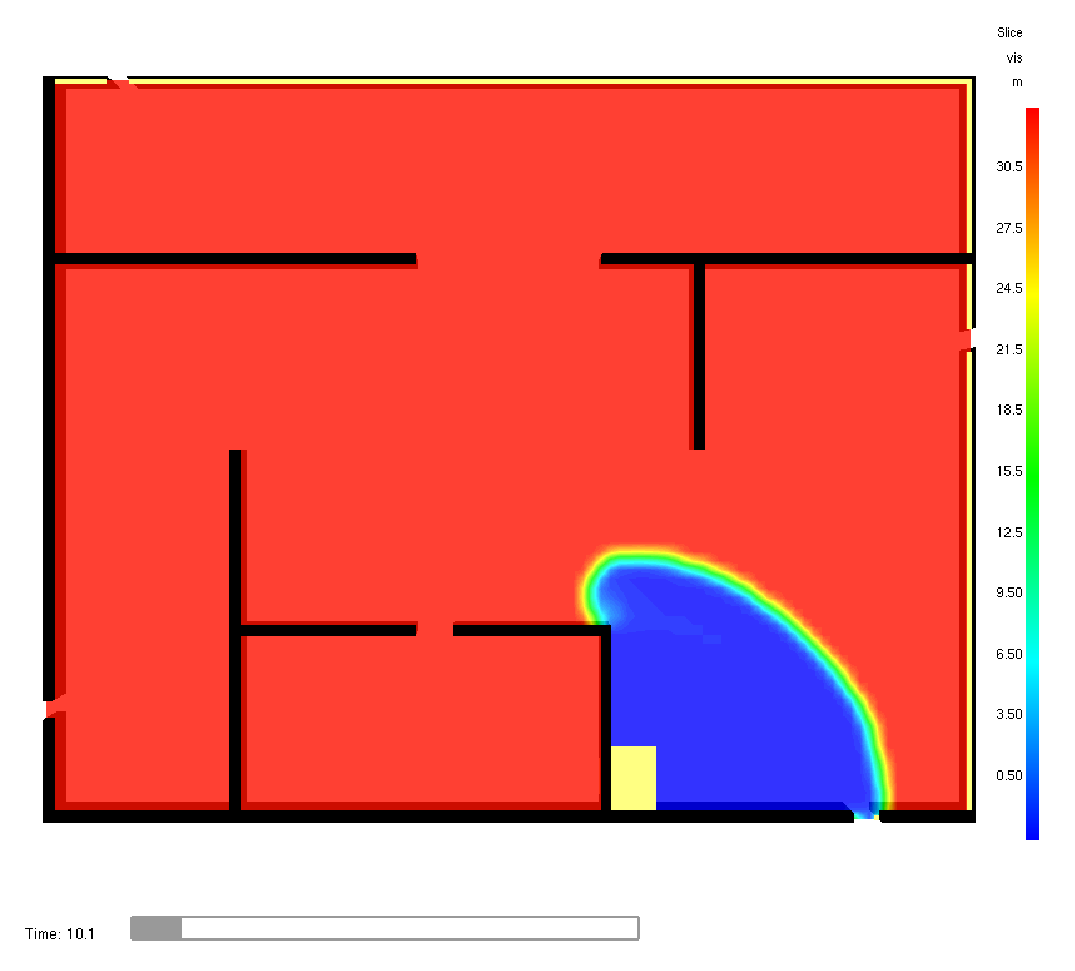
\includegraphics[clip=true,width=80mm]{DoorTestSmokeDens.eps}}
  \caption{The visibility at 10 s in the test case. Red and blue
    colours indicate good and very bad visibilities,
    respectively.}\label{Fig_ExitDoorSmokeDens} 
\end{figure}
%

%
\item Decision making model without smoke: The verification of the
  exit door selection algorithm of FDS+Evac was tested using the
  geometry shown in Fig.~\ref{Fig_ExitDoorNoSmoke}.  The figure on the
  left shows the target exit doors for the agents (blue: right bottom
  exit; green: top left exit) and in the figure on the right the
  colours of the agents mark the preference categories of the exit
  door selection algorithm (black: known visible door; yellow: known
  nonvisible door).  This test case has no smoke and as a result,
  agents use only the known doors (top left and bottom right ones).
  The doors on the left and right walls are not used, because they are
  not defined as ``known doors'' in the input.
  Figure~\ref{Fig_ExitDoorNoSmoke} verifies that the door selection
  algorithm works as intended when there is no smoke.  Agents first
  choose the nearest visible known door, if such exists.  If there are
  no visible doors, the agents choose the nearest nonvisible but known
  door; see \emph{e.g.} the agents in the bottom left corner of the
  building.  Note however, that in the present version of FDS+Evac,
  the distance to the nonvisible doors is calculated along a straight
  line through the internal walls.  In later versions, the algorithm
  may be changed to calculate the distance along the streamlines used
  to guide the agents towards the doors.

%
\item Decision making model with smoke: The above test was modified by
  adding a fire that produces smoke to the building.
  Figure~\ref{Fig_ExitDoorSmokeDens} shows the visibility at the
  height of the human eyes at 10~s from the ignition.  The door
  selections and preference categories at the same time are shown in
  Fig.~\ref{Fig_ExitDoorSmoke}.  Now the smokiness has changed the
  preferences.  First choices are still the doors with no smoke.  The
  input files for the exit selection tests are on the FDS+Evac web
  page an interested reader is able to rerun the simulations and use
  Smokeview to see that the door selection algorithm is functioning
  like intended.

%
\begin{figure}[!tb]
  \centerline{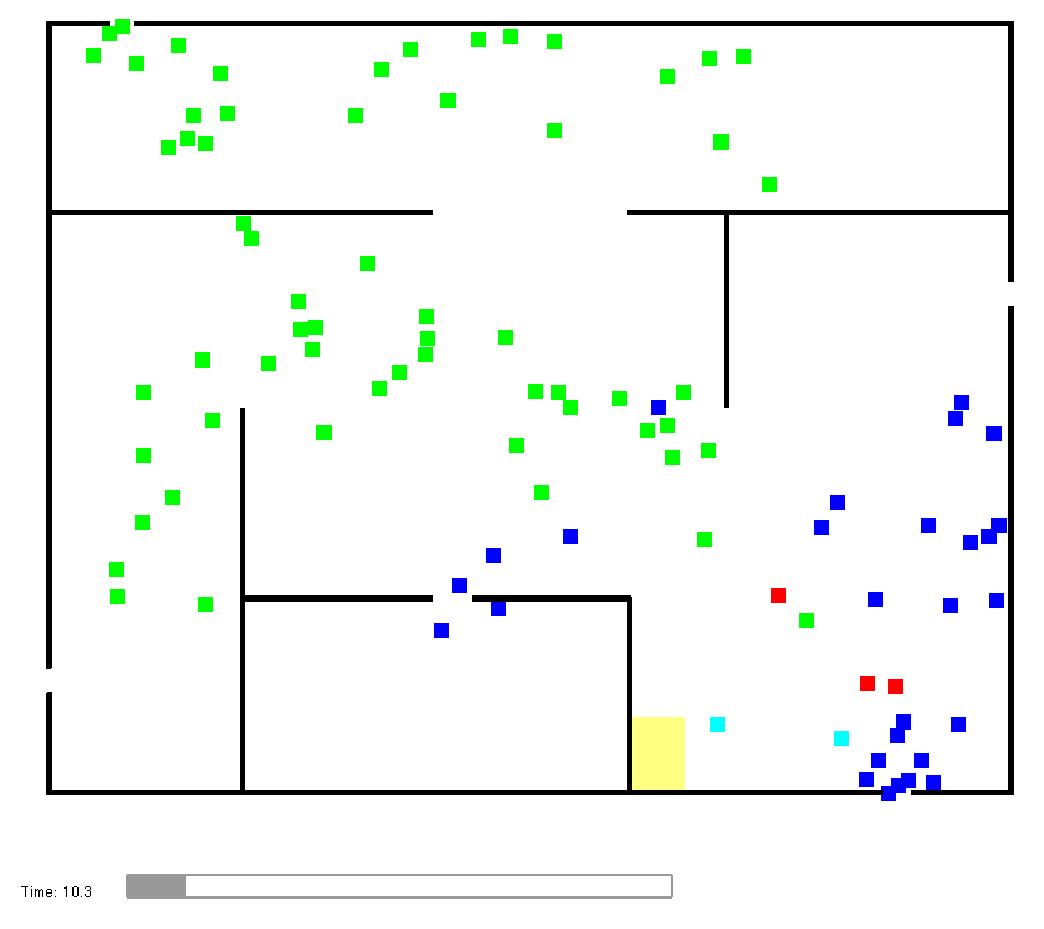
\includegraphics[clip=true,width=60mm]{DoorTestSmoke_Doors.eps}
  x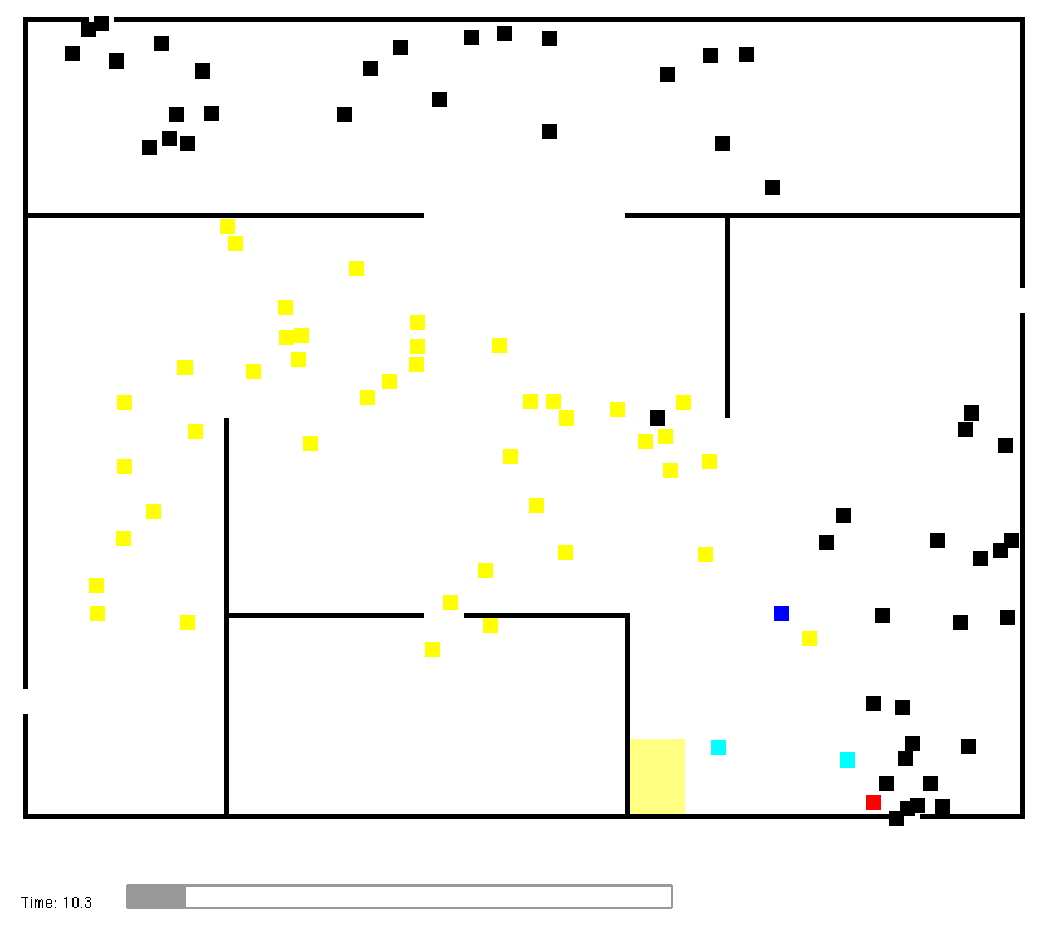
\includegraphics[clip=true,width=60mm]{DoorTestSmokeAlgorithm.eps}}
  \caption{An exit door selection test with
    smoke.  On the left, agents are coloured according to their exit
    doors. On the right, they are coloured according to their current
    preference categories.}\label{Fig_ExitDoorSmoke}
\end{figure}
%
%
%
%\item CORR and walking speed: CORR and EVSS stairs with many different
%  ways: TO DO
%
\end{enumerate}
%


\subsection{Numerical Tests}\label{Sec_NumTest}


%
%\begin{enumerate}
%
%\item Time step tests: TO DO
%
%\end{enumerate}
%



\section{Model Sensitivity}\label{Sec_ModelSensi}

\subsection{Introduction}

This section concentrates on the effects of different input parameters
on the outputs.  Especially the flows through doors, corridors and
stairs are examined, because these are usually the main bottlenecs of
an evacuation of a building.  This section does not address the point
if the chosen algorithms, numerical methods, etc. are appropriate for
the evacuation simulation or not.  Only the sensivity of the chosen
algorithms and numerical methods are examined and reported.

\subsection{Grid Sensitivity}\label{Sec_GridSensi}

In principle, the algorithm described in Sec.~\ref{Sec_BasisModel}
does not have any underlaying grid.  It is continuous in time and
place.  But the implementation of the method in FDS+Evac introduces
computational grids.  These grids are used to define the geometry of
the calculation.  The most obvious grid sensivity issue is that the
resolution for the obstructions, like doors, stairs, etc., is the grid
resolution.  The other, subtler effect is the way how the grid
resolution changes the evacuation flow fields used to guide humans to
the exit doors.  In some cases, a finer grid does always mean a better
guiding field for humans.  If the evacuation grid resolution is much
less than the half of the body dimension then one may find some
difficulties to obtain nice evacuation flow fields, see the IMO test
case 10 in~\ref{Sec_QualVerif}.

The FDS fire calculation grid has effects on the evacuation
calculation via the smoke, toxic gas, temperature, and radiation level
calculation.  How accurate are the predictions of FDS for the fire
products will, of course, depend on the FDS grid resolution.  See the
FDS Technical Guide for the effects of the grid resolution on the FDS
fire calculation.  The evacuation calculation interpolates the fire
calculation results to the 2D evacuation grids and the evacuation grid
resolution will have an effect on the spatial accuracy of this fire
related information, but usually grid sizes are equal or less than the
dimensions of a human body and, thus, the accuracy of the fire
information in the evacuation grids is fine enough.

% Tests: 1.0, 1.5, 2.0m doors, dx=dy=0.05,0.10,0.20,0.50m

%T�nne muutetaan evac gridien dx,dy ja katsotaan, ett� vaikuttaako
%tuloksiin.  Tietenkin vaikuttaa, sill� oviaukkojen leveys muuttuu
%gridin mukana, mutta t�m� on tiedossa, eli laskee sill� geometrialla,
%mik� n�kyy Smokeviewlla.  Muuten ei ole gridista paljoakaan riippuva
%eli gridi riippuvuus tulee geometrian kautta.



\subsection{Human Parameter Sensitivity}\label{Sec_HumParSensi}

%
\begin{figure}[!tb]
  \centerline{ 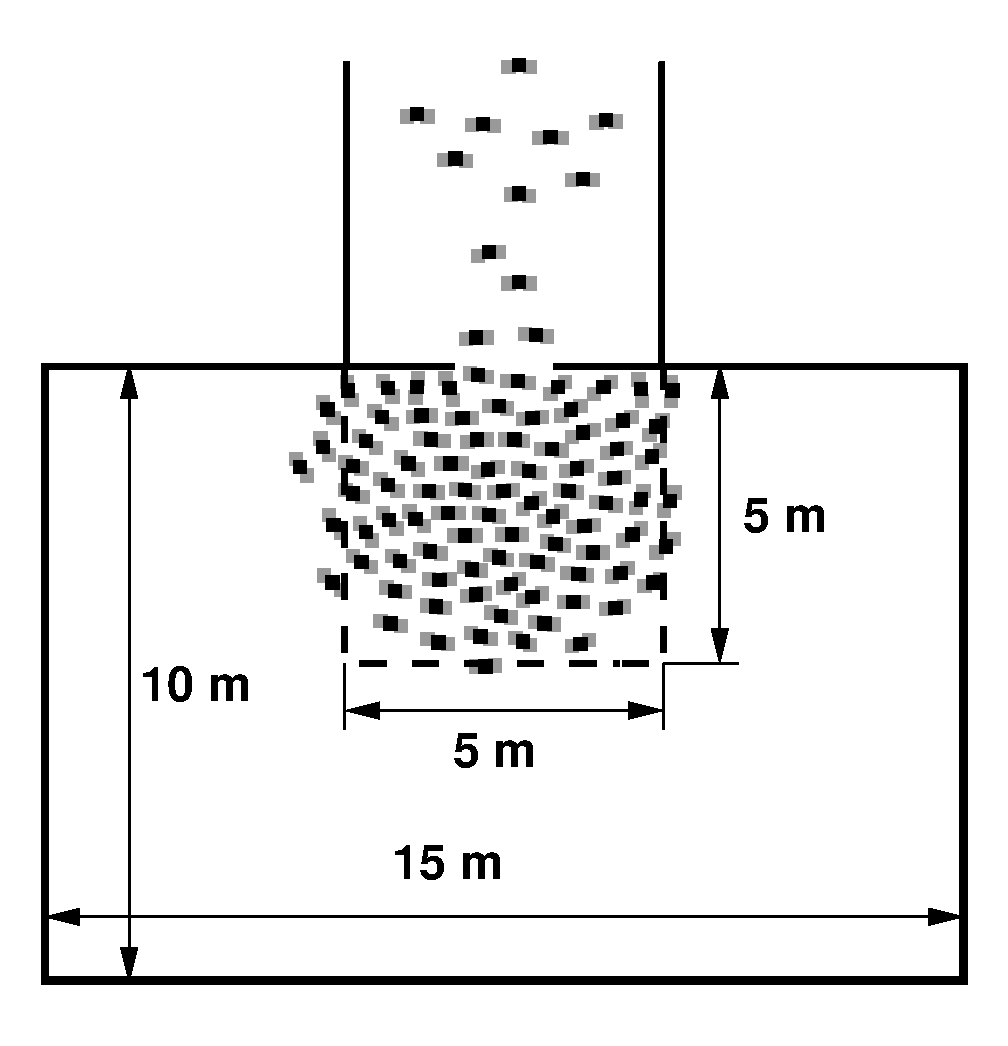
\includegraphics[clip=true,
    width=60mm]{./Door_Geom.eps} ~~~~~~~~   
    \includegraphics[clip=true,width=60mm]{./CorrGeom2.eps} }
  \caption{Test geometries used to calculate the specific flows through
    doors and corridors.\protect\hspace{200mm}}\label{Fig_Geoms}
\end{figure}
%

The human movement algorithm of FDS+Evac has many parameters.  Some of
these are related to the physical description of humans, like the body
size, the mass, the walking speed, and the moment of inertia.  The
others are the parameters of the chosen movement model, $\tau$,
$\tau^z$, $\omega^0$, the parameters of the social force, $A$, $B$,
$\lambda$, and the parameters of the contact force, $k$, $\kappa$,
$c_d$.  To test the relative importance of these parameters, Monte
Carlo simulations were performed to find the parameters which have the
greatest effect on human flows.  Two different geometries were used in
the simulations, see Fig.~\ref{Fig_Geoms}. One of the geometries was
used to study the flow of humans through a narrow door and through a
wide door and the other geometry was used to study human flows in a
corridor using densities 1.0 and 2.0 persons per square metre.  There
were 100 humans randomly located at the $5 \times 5 ~\mathrm{
  \textrm{m}^\textrm{2} } $ square in the door flow calculations.
Corridor flow calculations had 96 or 192 humans inside the corridor
depending on the density.  Thousand egress simulation with different
random initial human properties were performed for each of these four
different cases.  In total eleven model parameters, $A_i$, $B_i$,
$\lambda_i$, $v^0_i$, $\tau_i$, $A_w$, $B_w$, $\lambda_w$,
$\omega^0_i$, $\tau^z$, and $I^z_{i}$, whose values were varied $\pm
20~\%$ using uniform distributions.  The monitored output quantity was
the specific human flow in all cases and the Spearman's rank
correlation coefficients (RCC) were calculated for these four cases
and they are shown in Fig.~\ref{Fig_RCC}.

%
\begin{figure}[!tb]
  \centerline{ 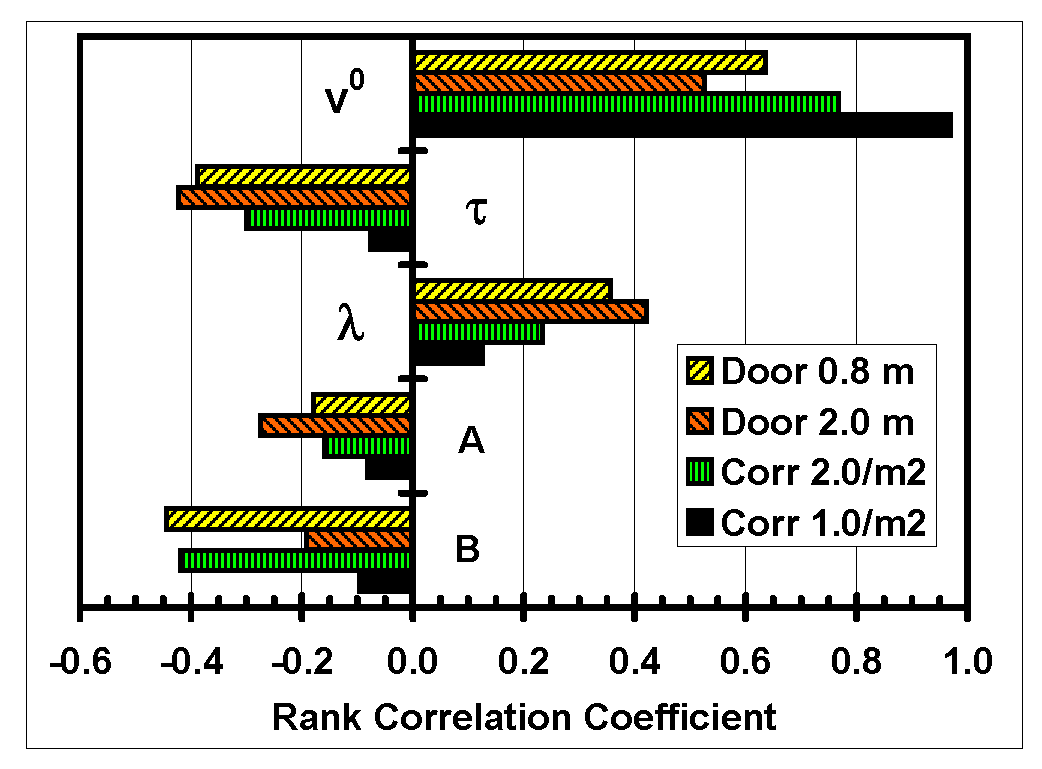
\includegraphics[clip=true, width=75mm]{./RCC_DoorCorr_new1.eps} ~~
               \includegraphics[clip=true, width=75mm]{./RCC_DoorCorr_new2.eps} }
  \caption{Rank correlation coefficients (RCC) for specific flows through
    doors and corridors. Widths 0.8~m and 2.0~m were used for doors
    and human densities 1.0~$\mathrm{ \textrm{m}^\textrm{-2} } $ and
    2.0~$\mathrm{ \textrm{m}^\textrm{-2} } $ were used for
    corridors.\protect\hspace{200mm}}\label{Fig_RCC}
\end{figure}
%

%
\begin{figure}[!tb]
  \centerline{ \includegraphics[clip=true, width=50mm]{./DoorCorr_Anew.eps} 
  \includegraphics[clip=true, width=50mm]{./DoorCorr_Bnew.eps}
  \includegraphics[clip=true, width=50mm]{./DoorCorr_Lambdanew.eps} } 
  \centerline{ \includegraphics[clip=true, width=50mm]{./DoorCorr_v0new.eps} 
  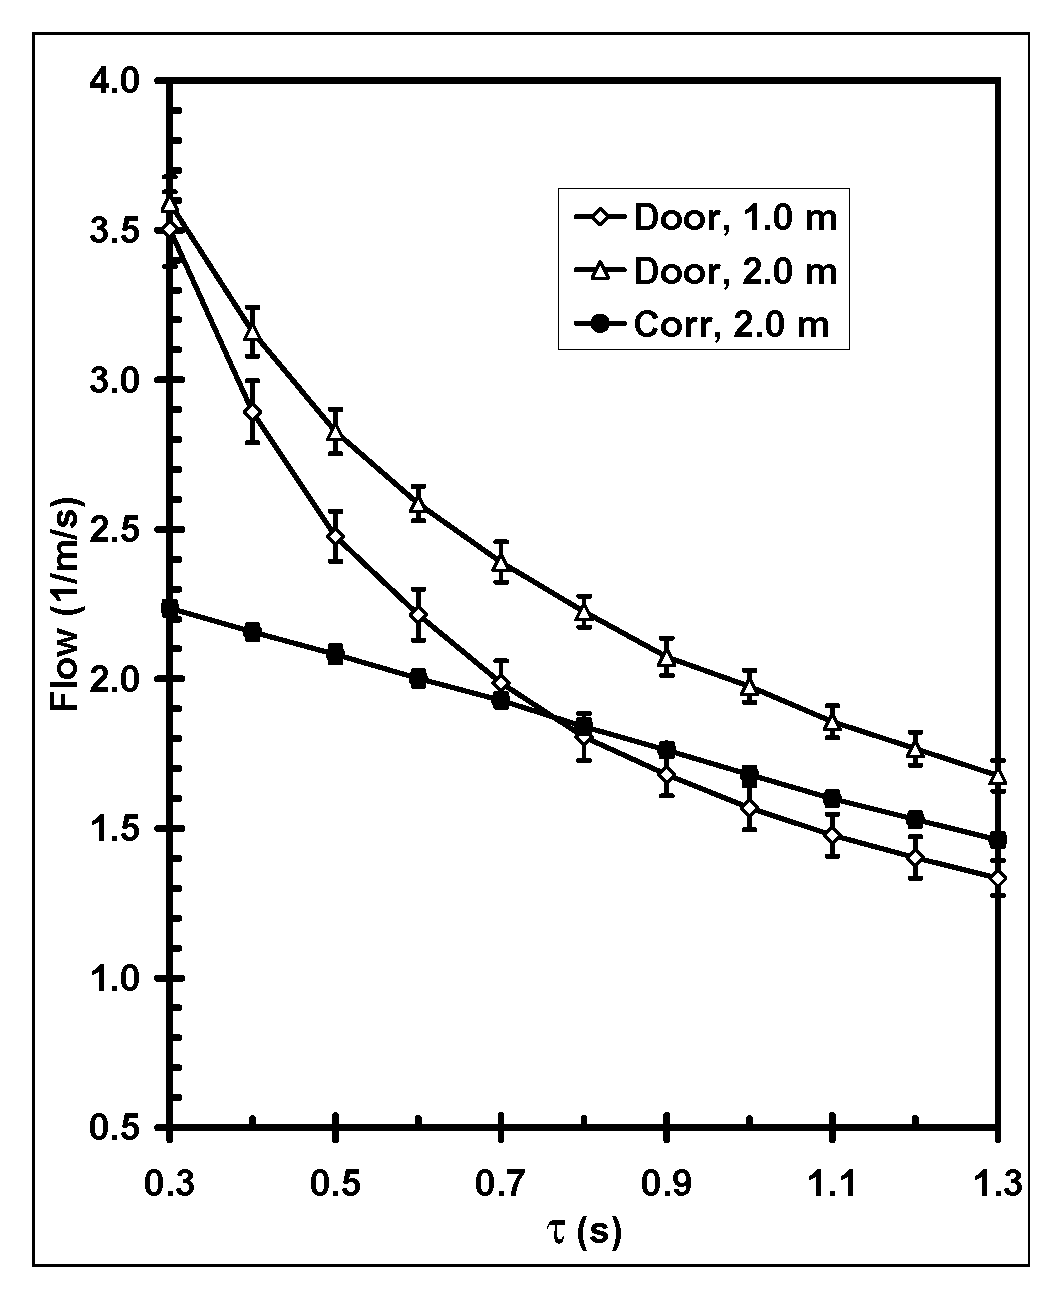
\includegraphics[clip=true, width=50mm]{./DoorCorr_Taunew.eps}
  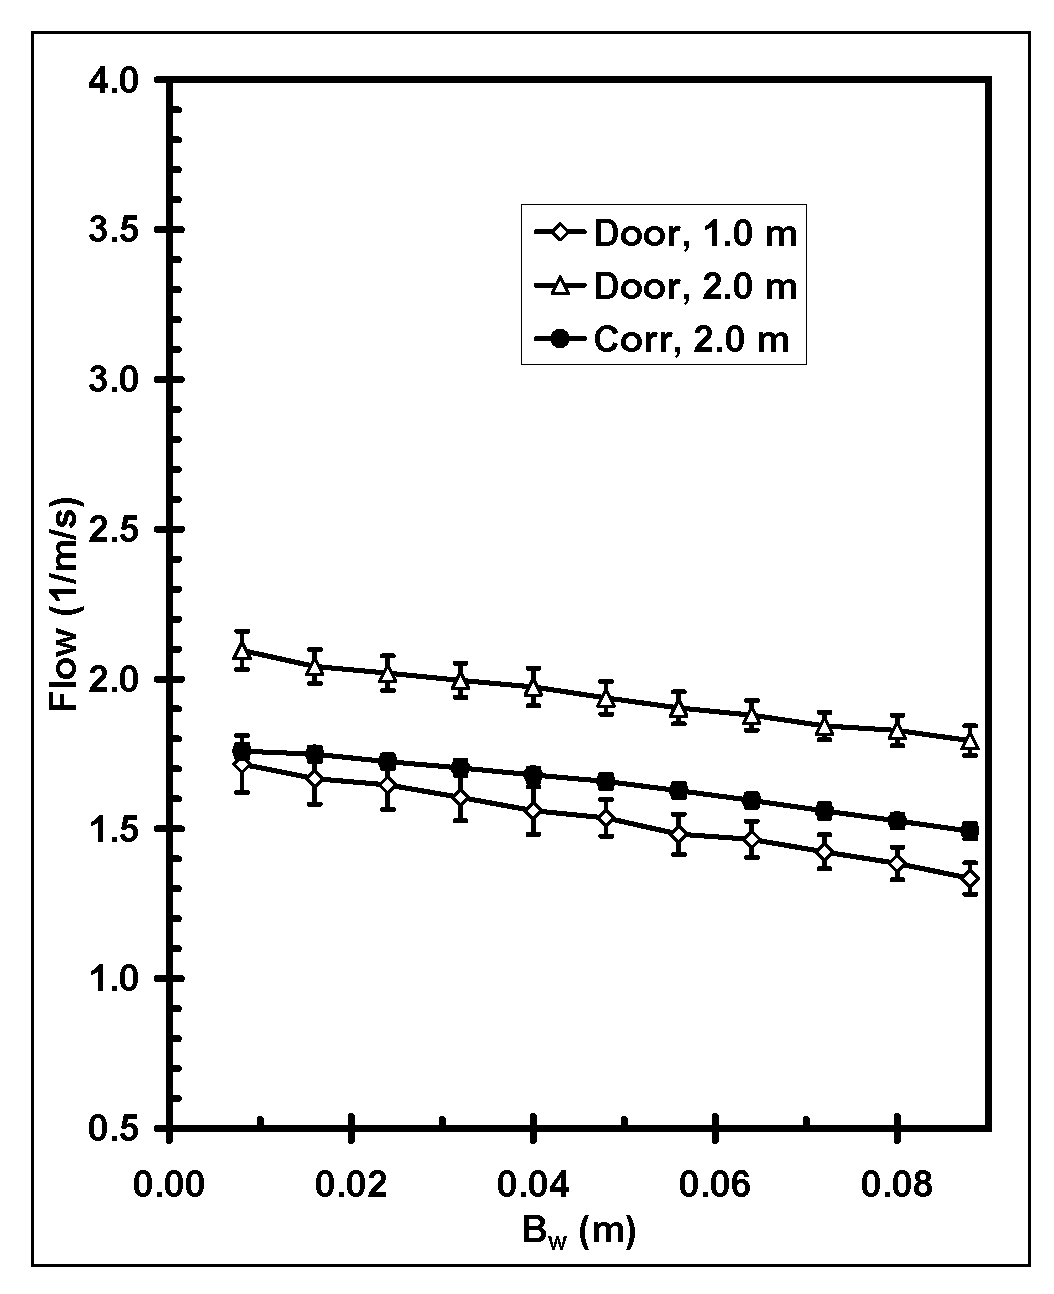
\includegraphics[clip=true, width=50mm]{./DoorCorr_Bwallnew.eps} } 
  \caption{Effects of different model parameters, $A_i$, $B_i$,
    $\lambda_i$, $v^0$, $\tau_i$, and $B_w$ on the specific flows
    through doors and corridors.  The corridor has 2.0~$\mathrm{
      \textrm{m}^\textrm{2} } $ human density and two doors widths,
    1.0~m and 2.0~m, are used.
    \protect\hspace{200mm}}\label{Fig_Door1}
\end{figure}
%

It is seen from Fig.~\ref{Fig_RCC} that the parameters $A_i$, $B_i$,
$\lambda_i$, $v^0_i$, $\tau_i$, and $B_w$ have the largest impact on
the specific flows through doors and corridors. Thus, further
simulations were done to quantify these effects. Each of these six
parameters were varied separately and 100 simulations were done for
each discretely chosen value of the parameters.  Two different door
widths, 1.0~m and 2.0~m, were chosen to represent a narrow and a wide
door.  Corridor flow was calculated using a density of 2.0 persons per
square metre, because it is known that around this density the
specific flow has its maximum value.  The results of these, in total
almost 20000 simulations, are shown in Fig.~\ref{Fig_Door1}, where the
markers represent the average of 100 simulations and standard
deviation is shown as error bars.  Note that in FDS+Evac the initial
properties and positions of humans are not deterministic, because the
humans are randomly positioned, the parameters $R_d$, $v^0$, and
$\tau_i$, are sampled from a random distribution and there are small
random forces in Eqs.~\ref{Eq_motion} and \ref{Eq_rotmotion}.
Increasing the values of $A_i$ and $B_i$ increases the social force
which tries to keep humans apart from each other and, thus, the
specific flow for door geometry will decrease.  The corridor case has
a constant human density.  Thus, these two parameters can not have an
effect through the density.  Larger social force, \emph{i.e.}, larger
$A$ and/or $B$, will make a forward walking person to reduce his/her
speed in order not to step on someone's heels, when the anisotropy
parameter, $\lambda_i$, is less than unity.  Increasing the walking
velocity will, of course, increase the specific flow.  Decreasing
$\tau_i$, \emph{i.e.}, increasing the motive force to go forward,
increases specific flows quite rapidly for the door geometry.  This
effect is not as pronounced in the corridor case, because there is no
free space in front of humans to accelerate and also the humans are
already moving with some velocity whereas they are almost standing and
waiting their turn in front of the door.  The anisotropy parameter of
the social force, $\lambda_i$, controls how eager humans are to push
those who are in front of them.  When $\lambda_i$ is large then humans
are 'pushy'.  The effect of the wall force parameter $B_w$ is to
modify the effective width of doors and corridors, thus, increasing
its value will make the effective width smaller and this will decrease
human flows slightly.

% T�h�n Asia-Oceania paperista kuvat

\subsection{Summary}

One should be very careful when constructing the geometry, where
humans are moving.  One should use Smokeview to see the human flow
fields before making a full evacuation simulation.

The effect of the parameters in the human movement algorithm,
Eqs.~\ref{Eq_motion}--\ref{Eq_motive_torque} are understood well and
user should usually not use any other than the pre-defined person
types in FDS+Evac.  The default pre-defined person types use a value
of 0.5 for the anisotropy parameter, $\lambda_i$, of the social
force.  For some application the resulting egress flows may be
considered to be too large.  If this is the case then the user should
use 0.3 as the value of $\lambda_i$.

% The grid resolution is used for the geometry.  One should avoid
% cases where the human flow fields are going through small, i.e.,
% less than human diameter, openings.


\section{Model Validation and Verification}\label{Sec_ModelValid}


\subsection{Introduction}



\subsection{Comparisons with Test Data}

%
%% \begin{figure}[!tb]
%%   \centerline{\includegraphics[clip=true,width=120mm]{CorrGeom2.eps}}
%%   \caption{The geometry used to calculate the specific human flows in
%%   corridors.}\label{Fig_CorrGeom} 
%% \end{figure}
%
\begin{figure}[!tb]
  \centerline{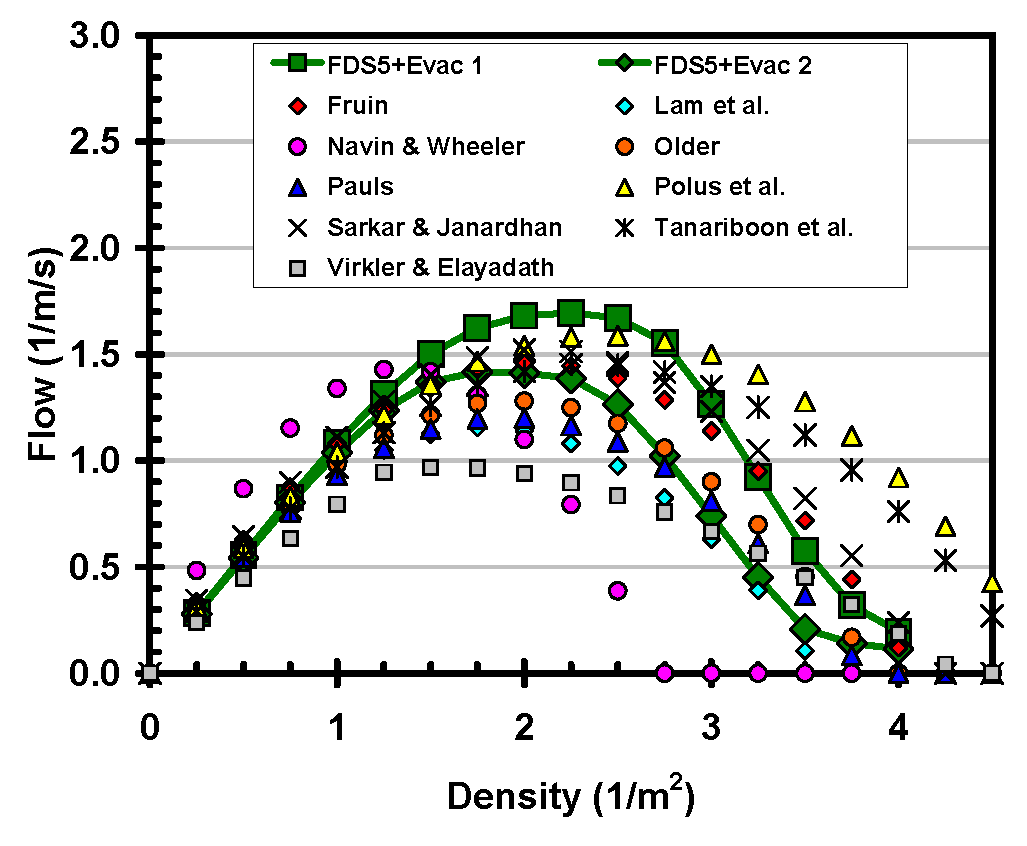
\includegraphics[clip=true,width=80mm]{CorrFlowResults.eps}}
  \caption{The specific human flows in corridors.}\label{Fig_CorrResults} 
\end{figure}
%

%
\begin{enumerate}
%
\item Specific flows through corridors: In the research of pedestrian
  flows, the dependence of the specific human flow rate on the human
  density is called as ``fundamental diagram''.  It shows how the
  specific flow first increases when the human density is increased,
  but then starts to decay as the density becomes high enough to
  hinder the walking.  In this test case, the specific flow rates
  given by the FDS+Evac code are compared to experimental walking
  velocities on horizontal floors in corridor geometry.  The geometry
  is shown in Fig.~\ref{Fig_CorrGeom}.  The corridor is modelled as a
  loop to avoid the effects of inflow and outflow boundary conditions.
  In Figure~\ref{Fig_CorrResults}, the predicted flow rates are
  compared against some experimental results for pedestrian traffic
  flows taken from Daamen's thesis~\cite{Daamen04}.  The FDS+Evac
  simulations were performed with two different parameter sets, labels
  ``1'' refer to the defaults of FDS+Evac and labels ``2'' refer to
  parameter sets, where $\lambda_i = 0.3$ is used. 

%
\begin{figure}[!bt]
  \centerline{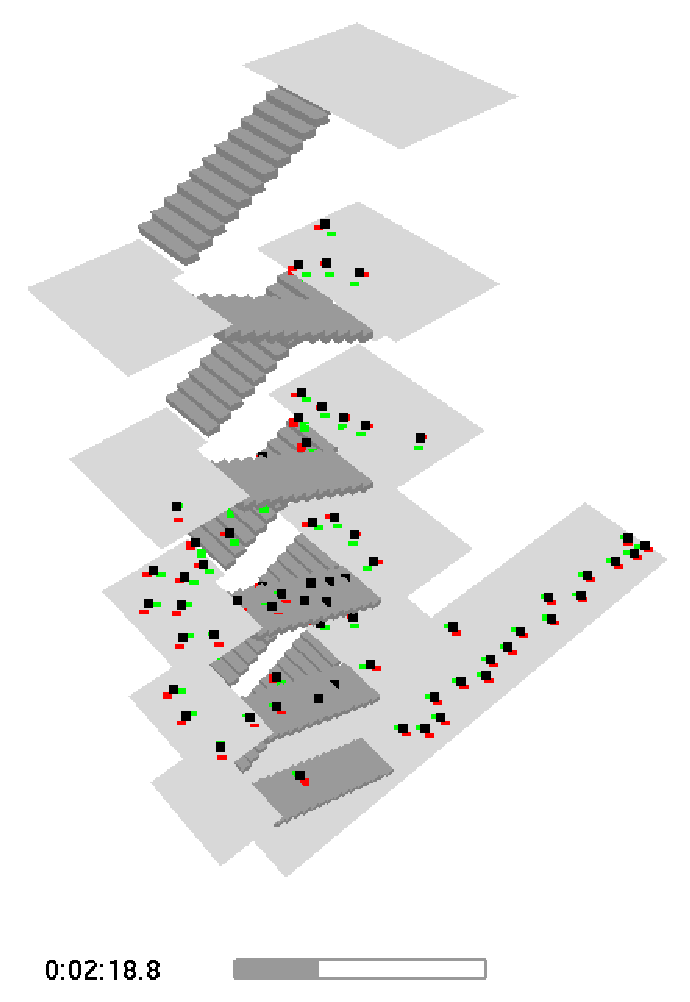
\includegraphics[clip=true,width=60mm]{PorrasKuva.eps}}
  \caption{A snapshot from a FDS+Evac simulation showing the geometry
  of the staircase.}\label{Fig_StairGeom} 
\end{figure}
%

%
\item Staircase of an office building: The evacuation experiment at
  the large office building~\cite{Hostikka2007a} was modelled using
  FDS+Evac.  Since the experiment was strongly focused on just one
  staircase, only this staircase was modelled.
  Figure~\ref{Fig_StairGeom} shows the geometry of the studied
  staircase.  The actual dimensions and door positions can be found in
  the experimental report~\cite{Hostikka2007a}.  The experimental
  entry times of humans to the stair landings were taken as inputs to
  the simulations.  The standard adult person type of FDS+Evac was
  used in the simulations.  Two different values were used for the
  anisotropy parameter of the social force, $\lambda_i=0.5$ which is
  the default, and $\lambda_i=0.3$ which corresponds to more relaxed
  egress.  The calculations for staircases were performed using both
  models for staircases available in FDS+Evac.

%
\begin{figure}[!tb]
  \centerline{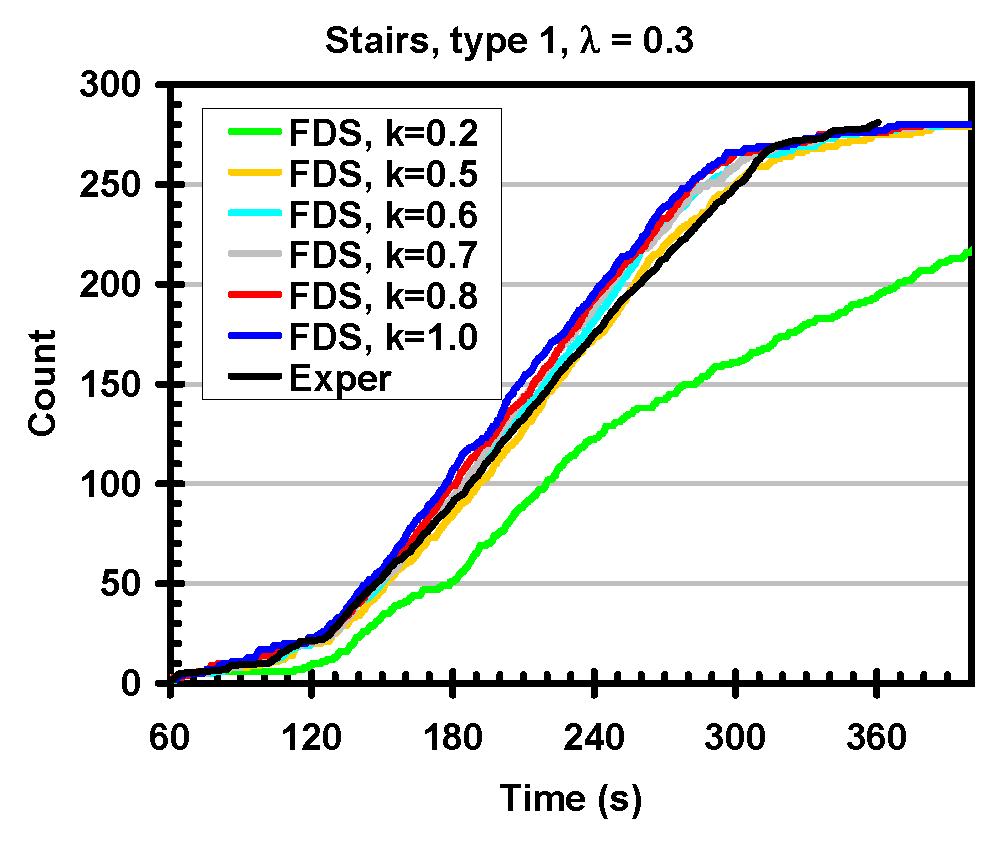
\includegraphics[clip=true,width=60mm]{StairsType1Lam0p3.eps}
  \includegraphics[clip=true,width=60mm]{StairsType1Lam0p5.eps}}
  \caption{Comparison of FDS+Evac (staircase model type 1) and experimental
    observations of a staircase flow.  Values 0.3 (upper) and 0.5
    (lower) for the anisotropy parameter of the social force are used.
    Different curves correspond to the different values of the
    staircase speed reduction parameter.}\label{Fig_StairType1}
\end{figure}
%

%
\begin{figure}[!tb]
  \centerline{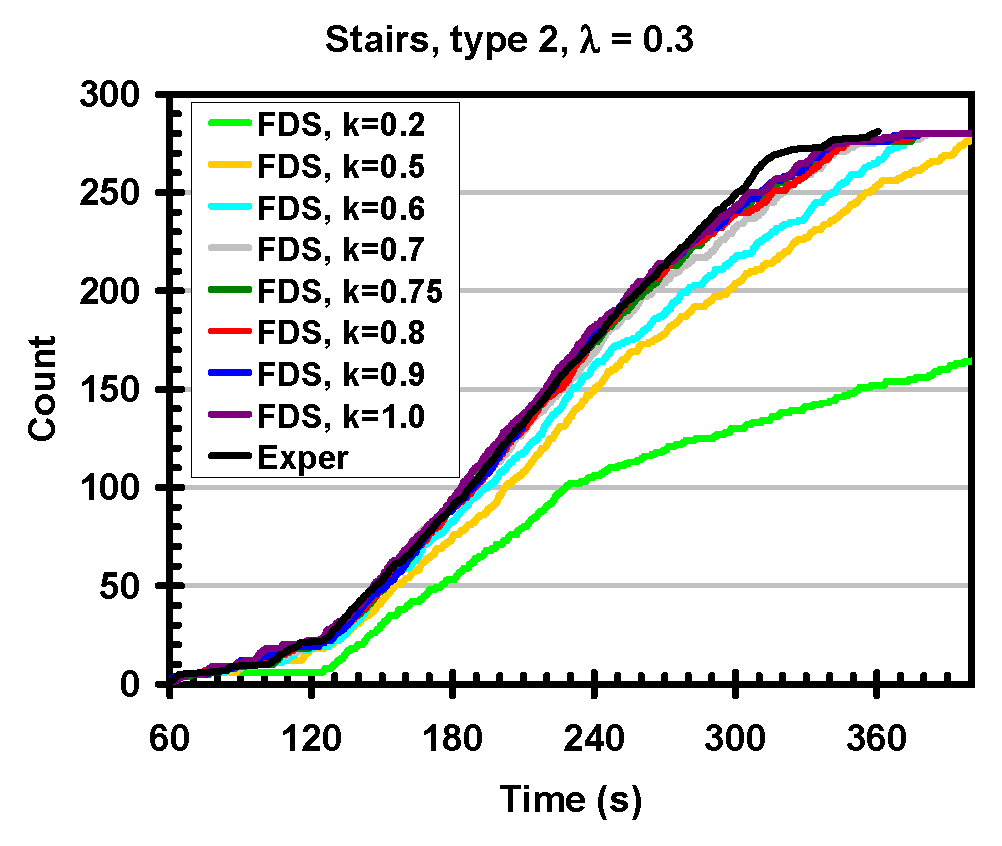
\includegraphics[clip=true,width=60mm]{StairsType2Lam0p3.eps}
  \includegraphics[clip=true,width=60mm]{StairsType2Lam0p5.eps}}
  \caption{Comparison of FDS+Evac (staircase model type 2) and experimental
    observations of a staircase flow.  Values 0.3 (upper) and 0.5
    (lower) for the anisotropy parameter of the social force are used.
    Different curves correspond to the different values of the
    staircase speed reduction parameter.}\label{Fig_StairType2}
\end{figure}
  
  Figure~\ref{Fig_StairType1} shows a comparison of the experimental
  observations and the simulation results using the simple staircase
  model (type 1).  This model is implemented using the \Timtt{\&CORR}
  namelist, which is a crude model for stairs.  In each figure,
  several simulated curves are shown corresponding to different values
  of the staircase speed reduction parameter.  In
  Figure~\ref{Fig_StairType1}, the best results are obtained when the
  value for the speed reduction parameter is 0.5, \emph{i.e.}, persons
  movement speed is reduced to $v = 0.5v_0$ inside the staircase.  The
  results using more sophisticated way of defining staircases (type 2)
  are compared to the observed values in Figure~\ref{Fig_StairType2}.
  In these simulations, the stairs are modelled as inclines where
  humans move at reduced speed.  Reducing the walking speed by a
  factor ~0.7 gives a good agreement with the observations.  Whether
  the anisotropy parameter $\lambda_i$ is 0.3 or 0.5 does not have any
  effect of practical importance.
%
%

\begin{figure}[!tb]
  \centerline{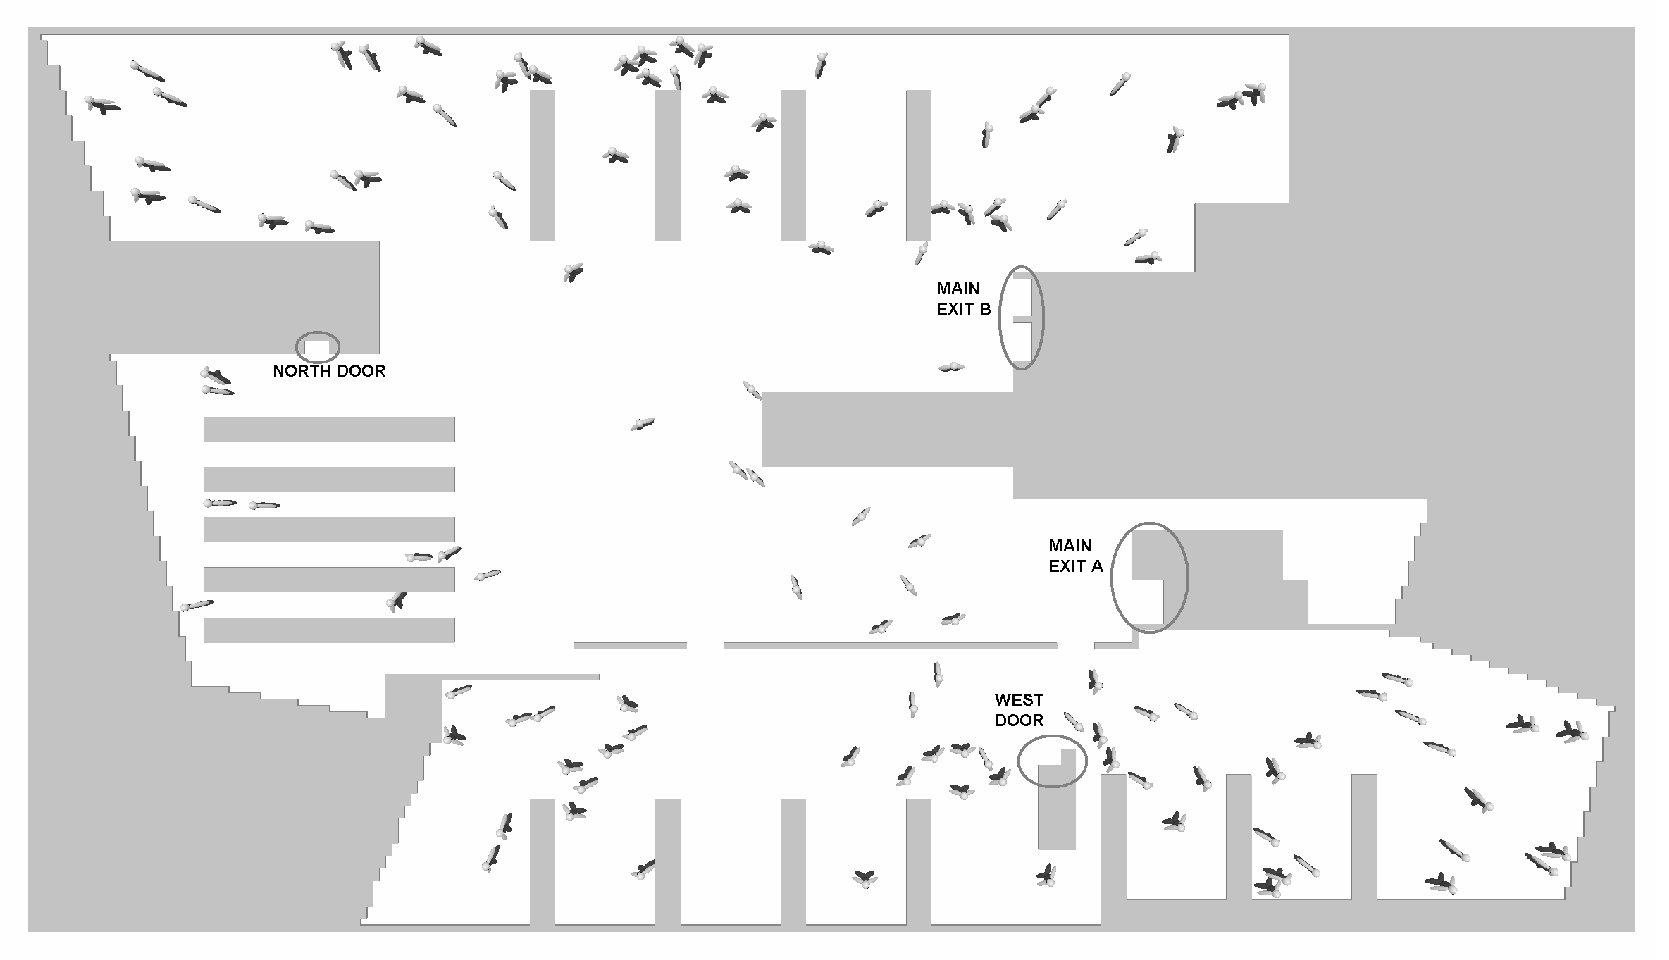
\includegraphics[clip=true,width=120mm]{Library_Kuva2.eps}}
  \caption{A snapshot from a FDS+Evac simulation shows the geometry of the
    FDS+Evac model for the second floor of the public
    library.}\label{Fig_Kirjasto}
\end{figure}

%
\item Public library: An observed evacuation experiment of the public
  library~\cite{Hostikka2007a} was simulated to study the capability
  to predict the entire movement phase of the evacuation, consisting
  of movement inside the floor, queuing to the staircase and finally
  movement through a narrow staircase to the exit.  The simulation
  geometry and the initial positions of the persons are shown in
  Fig.~\ref{Fig_Kirjasto}.  As the majority of persons in the building
  used the north exit door, the main results are for this door.  Shown
  are also the results for the west door, where about 50\% of the
  people originated from the first floor.  In the simulations, only
  the second floor of the building was simulated and people
  originating from the first floor were placed into the second floor.
  The north door was the only door with observed crowding.

%
\begin{figure}[!tb]
  \centerline{\includegraphics[clip=true,width=80mm]{KirjastoTulokset.eps}}
  \caption{Comparison of FDS+Evac simulation results and observations
    at the north and west doors of the public
    library.}\label{Fig_KirjastoResults} 
\end{figure}
  
  The decision making processes were not modelled.  Instead, the
  people were allocated for the north and west doors according to the
  ratio observed in the experiment.  The simulations were performed
  using FDS5+Evac and standard input parameters for the human
  properties.  The premovement times were generated from symmetric
  triangular distribution with mean of 31~s and lower and upper limits
  of 11~s and 71~s, respectively.  A comparison of the simulated and
  experimentally observed flows is shown in
  Fig.~\ref{Fig_KirjastoResults}.  As can be seen, the predicted flow
  rates are in very good agreement with the experiments.  For the west
  door, the results reflect the goodness or badness of the assumed
  premovement time distribution because the flow rate through the door
  is so small.  For the north door, the simulation is very relevant,
  because the flow rate is mainly determined by the geometry and the
  crowd dynamics during the queuing process.
%
%
\end{enumerate}
%

%Case 1: RI Nightclub: ToDo

%Case 2: Theatre at Tampere, Finland: ToDo

%Case 3: Stairs in an office building in Helsinki.

%% \subsection{Comparisons with Engineering Correlations}
%% See Section~\ref{Sec_HumParSensi}.
%% Stair flows, door flows, corridor flows. Here also comparison with
%% other evacuation models for these simple test geometries.

% ToDo: stair flows vs correlations

\subsection{Comparisons with Other Evacuation Models}

See the FDS+Evac web page, where the following test cases have been
reported.
%

%
\begin{figure}[!tb]
  \centerline{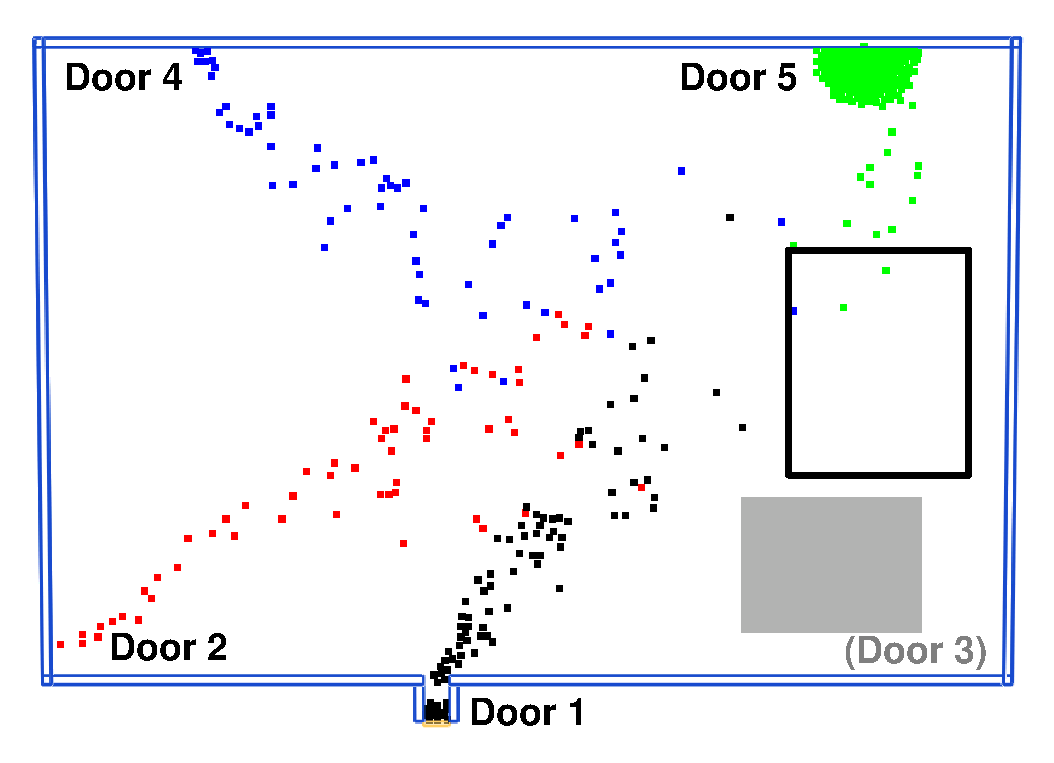
\includegraphics[clip=true,width=80mm]{eeri_n60s15_v1_114s.eps}}
  \caption{The geometry of the studied sports hall.  The open rectangle
    shows the area, where the agents are at the start of the
    simulations.  The gray rectangle shows the fire location, which is
    close to door 3 and, thus, this door is not
    used.}\label{Fig_SportGeom}
\end{figure}
%

%
\begin{figure}[!tb]
  \centerline{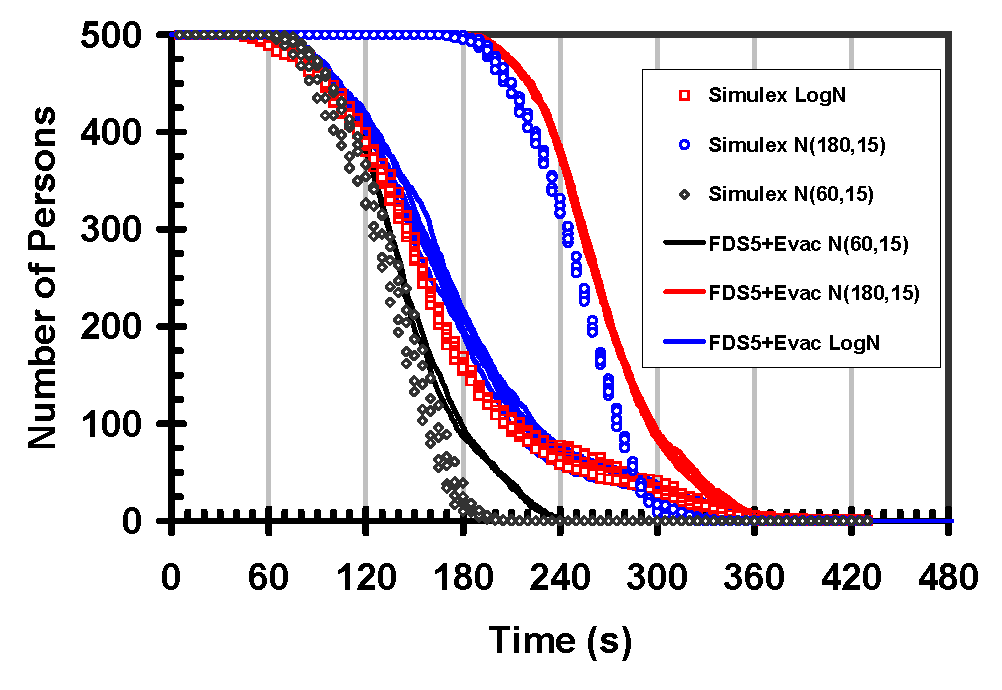
\includegraphics[clip=true,width=80mm]{EerikkilaResults.eps}}
  \caption{The comparison of FDS+Evac to Simulex in a sport hall
    case.  Results of five different simulations are shown for each
    case.}\label{Fig_SportResults}
\end{figure}
%

\begin{enumerate}
%
\item Sports hall: FDS+Evac simulations were compared to
  Simulex~\cite{Integrated96} simulations in a sports hall shown in
  Fig~\ref{Fig_SportGeom}.  The hall was previously analysed by
  Paloposki \emph{et al.}~\cite{Paloposki02}.  The sports hall is used
  to practice different kind of sports.  There are no spectator stands
  in the hall and neither are there any social spaces like showers.
  People enter the hall through the main entrance (``Door 1''), which
  is 1.8~m wide.  Doors 2 and 3 are 4.0~m wide two leaf doors and
  doors 4 and 5 are 0.9~m wide single leaf doors.  It is assumed that
  a fire starts close to door 3 (the shaded rectangle in
  Fig.~\ref{Fig_SportGeom}) so that this door cannot be used for
  egress.  235 persons use the closest door (``Door 5''), 130 persons
  use the main entrance (``Door 1''), 60 persons door 2, and 75
  persons use door 4.  Persons are initially located at the east end
  of the hall in an area of 20$\times$25~$\mathrm{m^2}$ (the open
  rectangle in Fig.~\ref{Fig_SportGeom}).  Three different reaction
  time scenarios were considered, two having a normal distribution
  with a standard deviation of 15~s but different means (60~s and
  180~s), and one having a lognormal distribution (median 75~s,
  standard deviation of the logarithm of reaction time was 0.7).
  Actually, the lognormal distribution was approximated by two uniform
  distributions, because the version of the Simulex, which was used,
  does not support lognormal distributions for the reaction time.
  
  The results of the simulations are shown in
  Fig.~\ref{Fig_SportResults}).  Since both FDS+Evac and Simulex are
  modelling human egress as a stochastic process, the presented
  results were collected from five different runs per case.  The
  FDS+Evac and Simulex results agree very well for the lognormal
  reaction time case, but for the other two cases the results differ
  somewhat.  These differences arise due to the ``Door 5'', which is
  only 0.9~m wide, but through which 235 persons escape.  The flow
  through this door is larger in Simulex than in FDS+Evac.  The
  specific human flow through this door in the FDS+Evac simulations
  are 1.65 1/p/m for the cases, where normal distributions were used
  for the reaction times.  The other doors are not as crowded and
  there the capacities of the doors do not show up as much.
%

%
\begin{figure}[!tb]
  \centerline{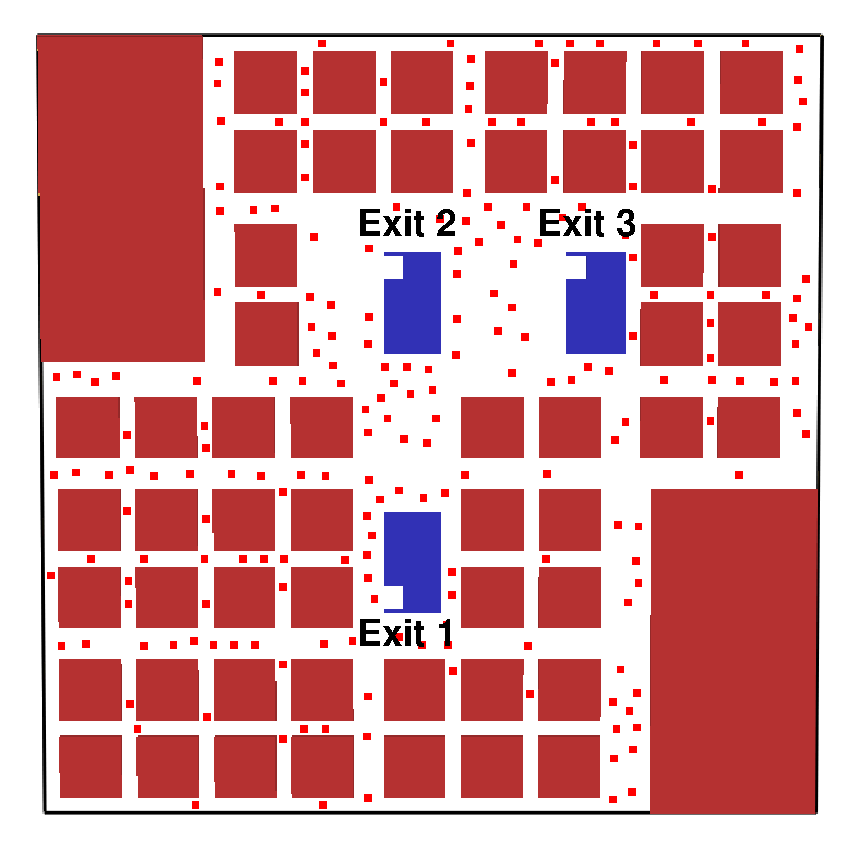
\includegraphics[clip=true,width=80mm]{b_ave90s11rnd_d123_initpos.eps}}
  \caption{The geometry of the open floor office test
    case.}\label{Fig_OpenFloorGeom}
\end{figure}
%

%
\begin{figure}[!tb]
  \centerline{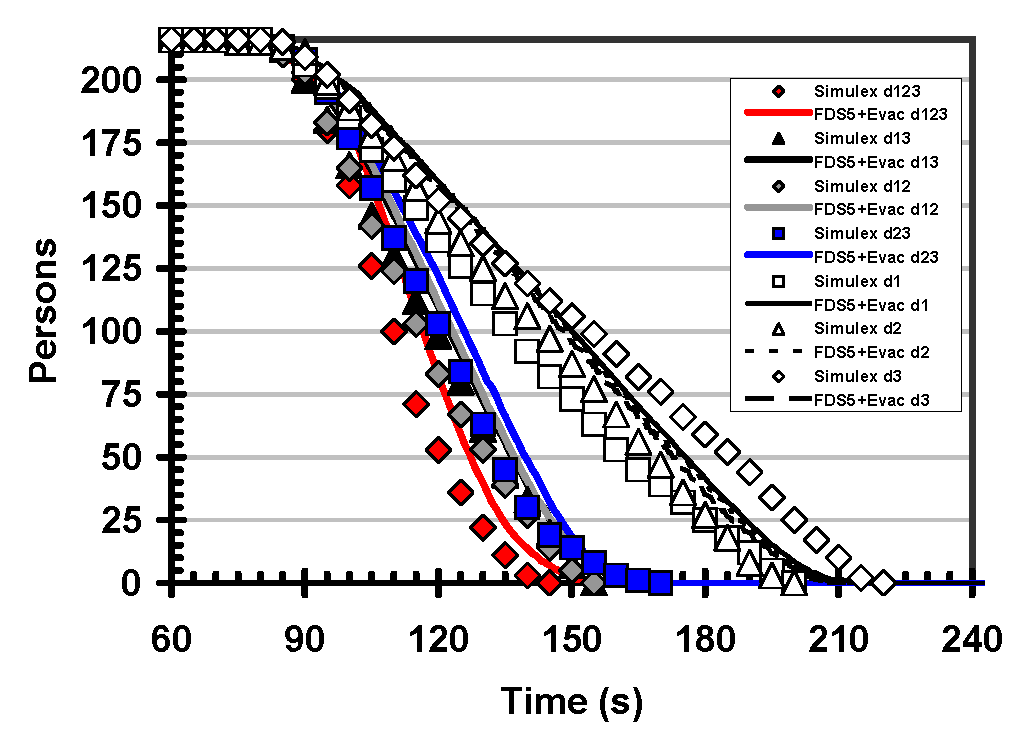
\includegraphics[clip=true,width=80mm]{PankkiTulokset.eps}}
  \caption{The comparison of FDS+Evac to Simulex in an open floor
    office case.}\label{Fig_OpenFloorResults} 
\end{figure}
%

\item Open floor office: This test geometry was an open floor office,
  whose floor plan is shown in Fig.~\ref{Fig_OpenFloorGeom}.  The
  floor has dimensions of 40$\times$40~$\mathrm{m^2}$ and there are
  initially 216 persons on this floor.  The properties of these humans
  were assumed to be as the ``Office Staff'' category in the Simulex
  model and the reaction times of the humans were assumed to follow a
  normal distribution with mean of 90~s and standard deviation of
  11~s.  There are three stairs located at the central core of the
  building.  The widths of the doors opening to the stairs are 1.2~m.
  In total seven different egress scenarios were simulated, covering
  the cases where all stairs are in use, one stair is blocked and a
  case where two stairs are blocked.
  
  The results of FDS+Evac simulations are compared to Simulex
  simulations in Fig.~\ref{Fig_OpenFloorResults}.  Only when two exit
  doors were blocked, queues were formed at the door.  For two or
  three operational doors the main form of the evacuation curves arise
  from the reaction time distribution.  The FDS+Evac and Simulex
  results are quite similar.  It should be mentioned, that in the
  FDS+Evac simulations, the initial (random) positions of humans do
  not change between different door scenarios (see
  Fig.~\ref{Fig_OpenFloorGeom}), whereas in Simulex runs the random
  initial positions are different in each calculation.  This explains
  why the Simulex results have larger scatter in the cases where a
  certain number of doors are operational.

%
\begin{figure}[!tb]
  \centerline{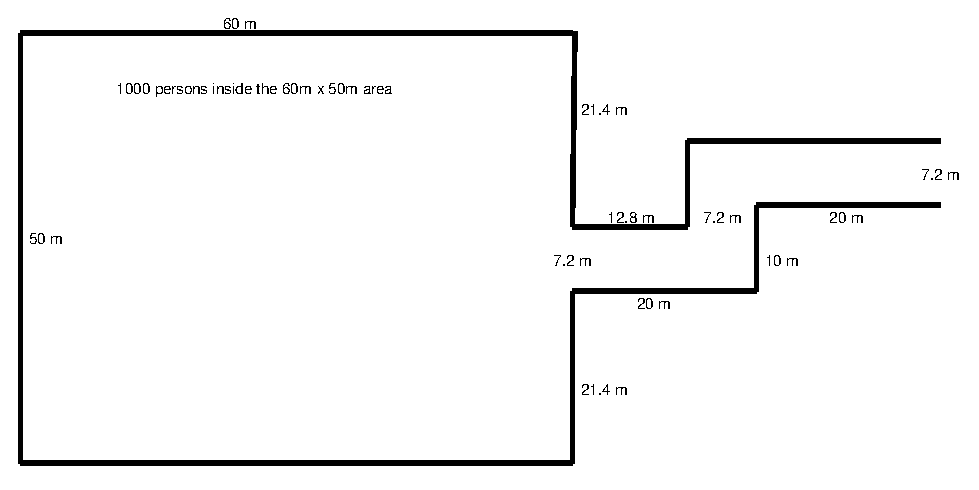
\includegraphics[clip=true,width=120mm]{Kaytava_fig.eps}}
  \caption{The geometry of the assembly space test
    case.}\label{Fig_AssemblyGeom} 
\end{figure}
%

%
\item Assembly space: The second test case is a large fictitious
  assembly space having dimensions of 50$\times$60~$\mathrm{m^2}$ and
  1000 people initially inside.  There is only one 7.2~m wide corridor
  leading to the exit.  The geometry is shown in
  Fig.~\ref{Fig_AssemblyGeom}.  The FDS+Evac results are compared to
  those of Simulex and buildingExodus~\cite{Thompson95} in
  Fig.~\ref{Fig_AssemblyResults}.  Note, that the FDS+Evac simulations
  were also done using parameters describing more relaxed egress
  (labels ``FDS+EvacSlow''), where the value of the anisotropy
  parameter of the social force, $\lambda_i$, had a value of 0.3.

%
\begin{figure}[!tb]
  \centerline{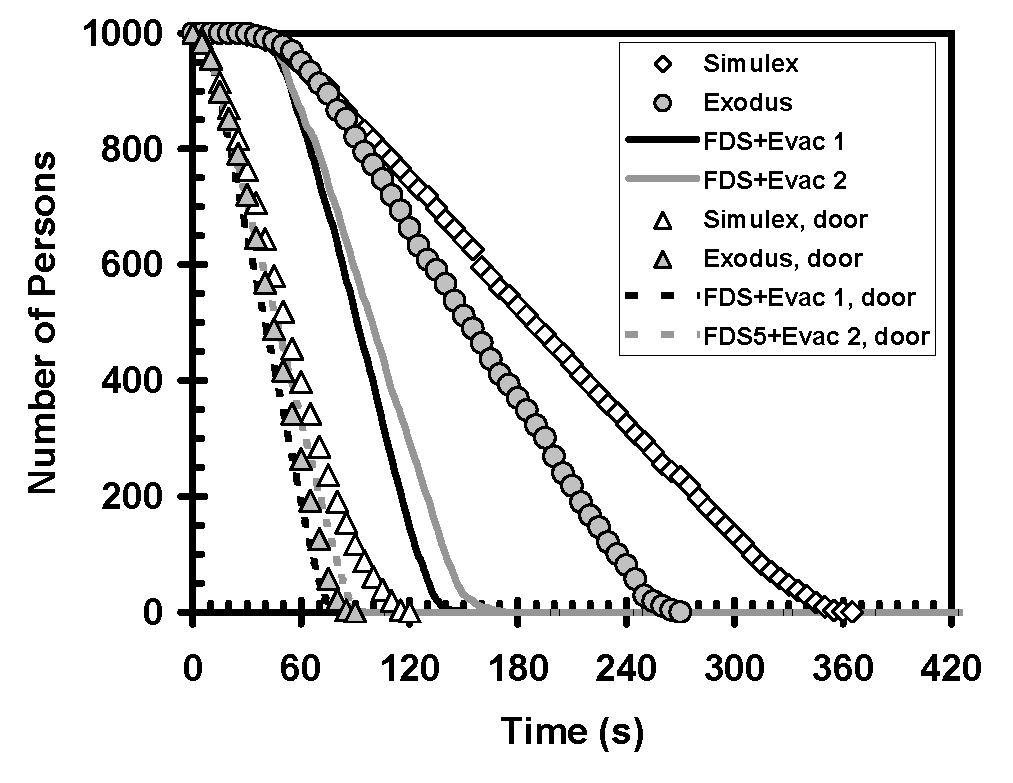
\includegraphics[clip=true,width=80mm]{KaytavaTulokset.eps}}
  \caption{The comparison of FDS+Evac to buildingExodus
    and Simulex in an assembly space.}\label{Fig_AssemblyResults}
\end{figure}
%

%
\begin{figure}[!tb]
  \centerline{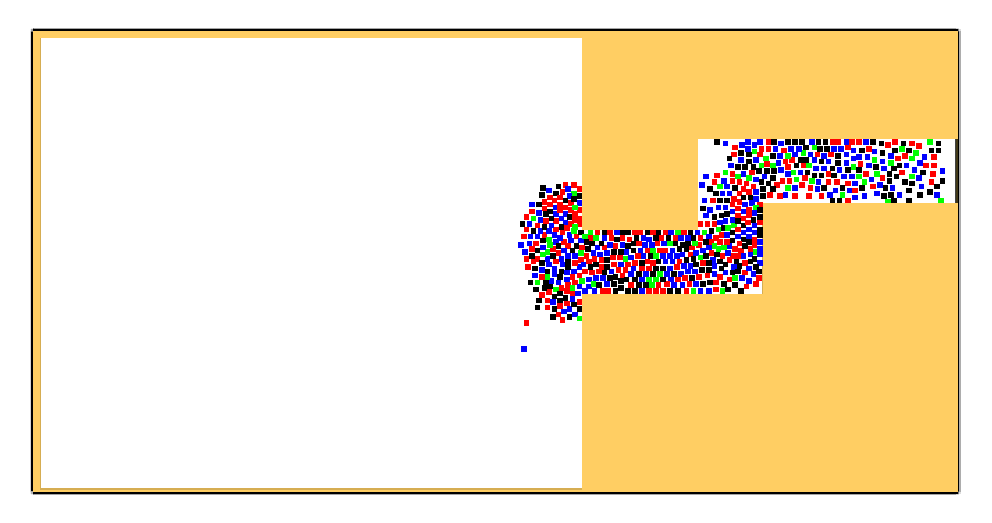
\includegraphics[clip=true,width=120mm]{kaytava_u1s0p5_65s.eps}}
  \centerline{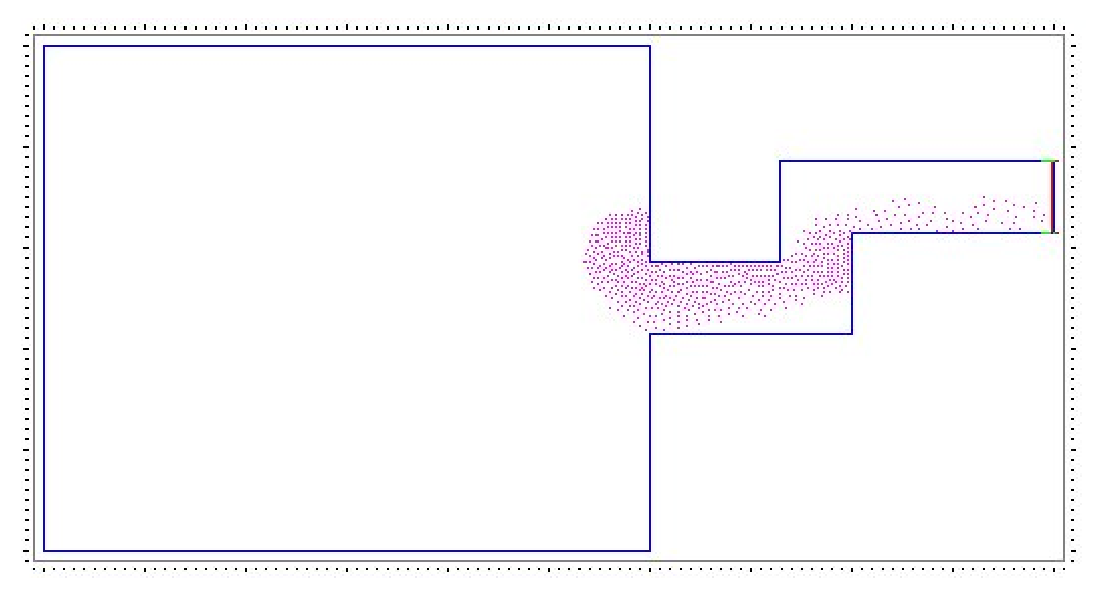
\includegraphics[clip=true,width=120mm]{kaytava_simulex120s.eps}}
  \caption{A snapshot from (a) FDS+Evac, (b) Simulex
    calculation}\label{Fig_AssemblySnapshots} 
\end{figure}
%
  
  Considerable differences are shown between the results of FDS+Evac
  and the results of Simulex and buildingExodus codes.  These
  differences can be traced back to the human motion in the corridor,
  see Fig~\ref{Fig_AssemblySnapshots}.  Simulex and buildingExodus are
  not using the whole width of the corridor efficiently, when the
  simulations are done using the default values and standard input.
  (An advanced user of these codes might be able to get different
  results by using some additional features.)  The results of FDS+Evac
  model look more realistic.
  
  In Figure~\ref{Fig_AssemblyResults} also shown are the results of
  the simulations for a case, where there is no corridor at all,
  \emph{i.e.}, there is just one 7.2m wide exit door located at the
  wall of the room.  In this case, the agreement between the different
  evacuation programmes is much better.  The calculated specific human
  flows (1/p/m) are: Simulex 1.44, Exodus 1.95, FDS+Evac 2.14 and
  FDS+EvacSlow 1.74 (~$\lambda_i =0.3$).

%
\item Specific flows through doors: The fourth test geometry is shown
  in Figure~\ref{Fig_DoorGeom}.  This geometry is commonly used in the
  literature to calculate the specific flows through doors.  In the
  test, there are 100 humans randomly located at the
  5$\times$5~$\mathrm{m^2}$ square.  In Figure~\ref{Fig_DoorResults},
  the results of FDS+Evac simulations for specific flows through doors
  are compared to simulation programmes Simulex and
  MASSEgress~\ref{Pan06}.  The results of the programmes MASSEgress
  and Simulex are extracted from Pan's thesis~\ref{Pan06}.  The
  FDS+Evac simulations are performed with two different parameter
  sets, labels ``1'' refer to the defaults of FDS+Evac and labels
  ``2'' refer to parameter sets, where $\lambda_i = 0.3$ is used.  It
  is seen that FDS+Evac is able to produce reasonable flows through
  doors.  For some applications, the flows generated by the default
  parameter values may be considered too large, but it is quite
  straightforward to modify the parameters of FDS+Evac to reach
  specific flows that are more relevant to a more relaxed egress.
%
%% \begin{figure}[!tb]
%%   \centerline{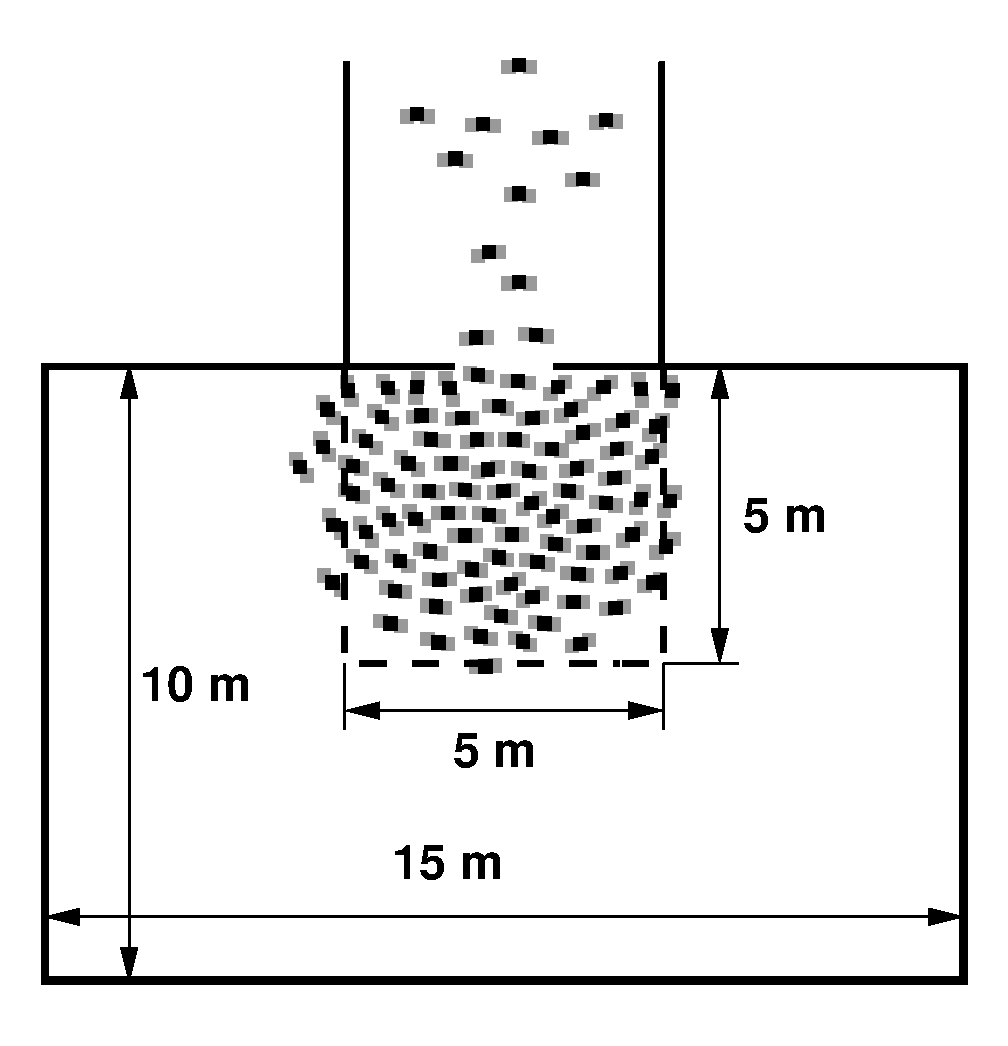
\includegraphics[clip=true,width=120mm]{Door_Geom.eps}}
%%   \caption{The test geometry used to calculate specific human flows
%%   through doors.}\label{Fig_DoorGeom}  
%% \end{figure}
%
%
\begin{figure}[!tb]
  \centerline{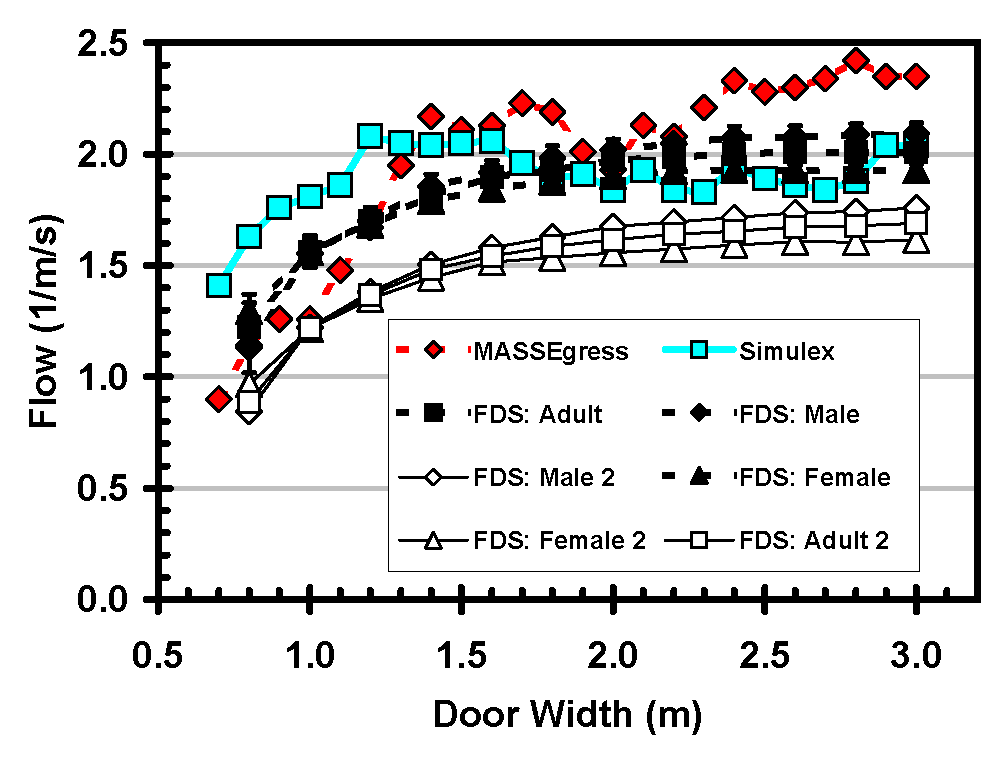
\includegraphics[clip=true,width=120mm]{OviFlowRersults.eps}}
  \caption{The specific human flows through doors.}\label{Fig_DoorResults}  
\end{figure}
%
%
\end{enumerate}
%

\clearpage



\section{Running FDS+Evac}\label{Sec_Running}

Running FDS+Evac is similar to running FDS, \emph{i.e.}, relatively
simple.  All of the parameters that describe a given fire and egress
scenario are typed into a text file that will be referred to as the
``fds'' or the ``input'' file.  In this document, the data file will
be designated as \textbf{CHID.fds}.  In practice, the user chooses the
ID string ``CHID'' so that all of the files associated with a given
calculation all have a common prefix.

In Section~\ref{Sec_SampleFile}, an example input file will be
presented.  Several other example files exists at the FDS+Evac web
site \verb+http://www.vtt.fi/fdsevac+.  It is suggested that a new
user start with an existing input file, run it as is, and then make
the appropriate changes to the input file for the desired scenario.
By running a sample case, the user will become familiar with the
procedure, learn how to examine the results, and ensure that his/her
computer is up to the task before embarking on learning how to create
new input files.

The FDS+Evac executable is the single CPU executable of the FDS,
fds5.exe.  A FDS+Evac simulation is run similarly as a FDS fire
simulation, so read the User's Guide of FDS~\cite{FDS_UserGuide},
where you can find information on how to run the model and see the
results by using Smokeview~\cite{SV_UserGuide}.  Assuming that an
input file called \textbf{CHID.fds} exists in some directory, the user
must run the program in a DOS
command shell as follows:\\
Open up a Command Prompt window, and change directories to where the
input file for the case is, then run the code by typing
\begin{verbatim}
    fds5.exe  CHID.fds
\end{verbatim}
to begin a run, which will output some text on the Command Prompt
window.  If the user wants to save the text output going on the
Command Prompt window, she/he should type
\begin{verbatim}
    fds5.exe  CHID.fds 2&>1 > CHID.err
\end{verbatim}
to begin a run.



\subsection{Updating an Existing FDS Input File to a FDS+Evac Input File}

\begin{itemize}
%
\item Make a FDS fire input file for your project and do the
  fire/smoke spread calculations using the single CPU version of the
  FDS executable.  Note, that the present version of the evacuation
  module demands that the fire part can be run using the serial
  version of FDS.  If the memory requirements of your fire calculation
  demand the use of the MPI version of FDS then you can not couple the
  evacuation calculation with the fire calculation, \emph{i.e.}, you
  can not use smoke and gas consentrations in the evacuation
  calculation.  If you are going to do run FDS+Evac only in the
  ``evacuation trial mode'' then the fire grids are not used and the
  memory requirements might not be as large, so you might be able to
  run just the evacuation calculation.
%
\item Save the fire input file to some other name (and change also the
  \Timtt{CHID} on the \Timtt{HEAD} namelist group).
%
\item Put a keyword \Timtt{EVACUATION=.FALSE.} to every \Timtt{HOLE}
  line, which you fire input has.  Make a copy of each \Timtt{HOLE}
  line which you want also to appear in the evacuation geometry and
  change \Timtt{EVACUATION} value to \Timtt{.TRUE.}  This may sound
  like a nuisance, but the way how FDS parses the input file demand
  that.
%
\item Add a line
  \verb|&SURF ID='OUTFLOW', VEL=+0.000001, TAU_V=0.1 /| to your input file.
%
\item Define meshes for the evacuation.  Each floor should have
  its own mesh.  The $z$ co-ordinate for these meshes should be at
  a level, where the most obstacles for the movement are, usually
  about one meter above the floor.  See Fig.~\ref{Fig_EvacGrid}
  and Sec.~\ref{Sec_EvacGrid}.
%
\item Put \Timtt{T=0.0} on the \Timtt{TIME} namelist group, comment
  out the fire meshes, \emph{i.e.}, remove ampersands at the
  beginnings of the fire mesh lines, and run FDS+Evac.  Use Smokeview
  to see, if the 2D geometry is looking right.  You can play around
  with the $z_\mathrm{min}$ and $z_\mathrm{max}$ to take the
  evacuation layout at different heights.
%
\item Define additional obstacles with \verb|EVACUATION=.TRUE.|, where
  you do not want humans walking.  No need to define \Timtt{SURF\_ID}
  for evacuation obstacles, because the default for these is
  \Timtt{INERT}.
%
\item Make additional holes with \verb|EVACUATION=.TRUE.|, where they
  are needed.  Usually these are needed at exits or doors.  See
  Fig.~\ref{Fig_DoorGeom} and Sec.~\ref{Sec_SpecFeatures}.
%
\item Run FDS+Evac (\Timtt{T=0.0}) and see if the 2D geometry is
  looking correct.  If not, correct it by adding more \Timtt{OBST}s
  and \Timtt{HOLE}s.
%
\item Define evacuation flow field vents (\Timtt{EVACUATION=.TRUE.,
    SURF\_ID='OUTFLOW'}) that suck fluid out of the evacuation meshes
  at the places where you want humans to go.  These vents should be
  placed at the doors and exits. Note, that in FDS5 vents should be
  defined on solid surfaces.  If you are using multiple human flow
  fields on a floor then you should specify the \Timtt{MESH\_ID} on
  the \Timtt{VENT} lines.  This specifies the evacuation mesh, where
  this vent is put.  Same applies to holes and obstacles as well, but
  usually one can use same obstacles and holes on each flow field.
  Remember to define slice output files at your evacuation mesh
  heights, e.g., \\
  \verb|&SLCF PBZ=x.x, QUANTITY='VELOCITY',VECTOR=.TRUE./|
%
\item Remove \Timtt{CHID\_evac.eff} file if it exists.  Run a short
  simulation, \emph{i.e.}, put \Timtt{T=1.0}.  Check the human flow
  fields by using Smokeview.  Check also that your evacuation geometry
  looks fine.  If not, add obstacles or holes to the evacuation
  calculation and remember to remove the \Timtt{CHID\_evac.eff} file.
  Repeat these steps as long as you are satisfied with the geometry.
  Note, that FDS+Evac tries to read the human flow fields from the
  disk if there exitst a \Timtt{CHID\_evac.eff} file.  This file
  should be recalculated each time when you make changes to the
  geometry by changing objects like \Timtt{OBST}, \Timtt{VENT},
  \Timtt{HOLE}, and \Timtt{MESH}.
%
\item Define your person classes, the \Timtt{PERS} namelist groups.
  These define the properties of the humans in the model.  Also the
  detection and reaction time distributions are given here.
%
\item Define your doors, exits, stairs, and entries, the \Timtt{DOOR},
  \Timtt{EXIT}, \Timtt{CORR}, and \Timtt{ENTR} namelists.  Activate
  meshes in Smokeview to see the actual positions of your obstacles in
  the evacuation meshes, which might be a little bit different than
  the values given in the input file due to the fact that FDS moves
  \Timtt{OBST}s, \Timtt{HOLE}s, and \Timtt{VENT}s to match the mesh
  cell boundaries.  See Sec.~\ref{Sec_SpecFeatures} and
  Fig.~\ref{Fig_DoorGeom} how doors should be defined.
%
\item Place the humans inside the building, the \Timtt{EVAC}
  namelists.  Use \Timtt{EVHO} namelists if needed.  Note, that humans
  should not be placed behind the exits or doors, but this is no
  problem, because exits and doors are usually defined on solid
  \Timtt{OBST}s.
%
\item Once again, run a short simulation.  See, that your humans have
  correct initial positions.  You can change the way how humans are
  shown in Smokeview by using the menu ``Show/Hide'' and choosing
  different ``Avatars''.  Note, that now you had the file
  \Timtt{CHID\_evac.eff} on your disk so this file was read in,
  \emph{i.e.}, the human flow fields were not recalculated and the
  calculation runs faster than before.
%
\item Run a longer simulation and see that the humans are moving
  correctly, \emph{i.e.}, they are following correct flow fields and
  the exits, stairs, and doors are working correctly.  Note that the
  reaction and detection time distributions given on the \Timtt{PERS}
  lines should be shorter than the simulation time to see some human
  movement. (pre-evacuation time = detection time + reaction time)
%
\item Do a full evacuation calculation and save the results, \emph{i.e.}, the
  CHID\_evac.csv file.  Repeat this step a dozen or so times.  Note,
  that the results are not exactly similar, because humans have random
  properties and initial positions.  These simulations correspond to a
  fire drill.  After this, activate the fire meshes, \emph{i.e.}, put the
  ampersands back to the fire mesh lines, and do a full FDS+Evac
  simulation.  Now the fire and evacuation simulations are done at the
  same time and a file \Timtt{CHID\_evac.fed} is written to hard disk.
  This file can be used to run many evacuation simulations per one
  fire simulation, \emph{i.e.}, no need to calculate the same fire for many
  times.  Note, that the CHID\_evac.eff file is (re)calculated always
  when there are active fire grids.
%
\item If you are doing more than one evacuation calculation per one
  fire scenario (as you should) then save the CHID\_evac.eff and
  CHID\_evac.fed files after the previous step, where fire and
  evacuation calculations were done at the same time.  Then comment
  the fire meshes out, \emph{i.e.}, the ampersands away once again, and rerun
  the case.  Copy the results (CHID\_evac.csv) to some other name and
  rerun once again, etc. For a given fire, you should run the
  evacuation part a couple of dozen times, because the FDS+Evac is not
  deternimistic model.  After the runs, examine the results: calculate
  averages, variances, etc.
%
\end{itemize}


\subsection{Getting Help, Error Statements, Bug
  Reports}\label{Sec_ErrorsBugs} 

%
\begin{itemize}
\item Send bug reports to: \Timtt{Timo.Korhonen@vtt.fi}.  The subject
  line should start with the characters \Timtt{FDS+Evac Bug:}.
%
\item Send help requests to: \Timtt{Timo.Korhonen@vtt.fi}.  The
  subject line should start with the characters \Timtt{FDS+Evac Help:}.
%
\item If the run stops early and the error message ``ERROR:
  Initialize\_Humans, Evac line \#, Mesh \#, i\_human \#'' is printed on
  stderr then the initialization of humans failed, \emph{i.e.}, FDS+Evac was
  not able to put the humans on the areas specified in the input file.
  Check that you are not trying to put too many humans on a too small
  area.  See the positions of those humans that FDS+Evac was able to
  generate by using Smokeview.  Note, that in some runs with the
  exactly input file you might get the error message and in some other
  runs not.  The reason for this is that FDS+Evac uses random numbers
  to generate the properties of humans and their initial positions.
%
\end{itemize}

\newpage


\section{Setting up the Input File for
  FDS+Evac}\label{Sec_EvacInputFile} 

This section is a short manual to the FDS+Evac program.  Read first
the FDS manual, because here only those features and keywords are
presented, which differ from the ordinary FDS fire input.  The
optional keywords are presented with a slanted typewriter font, like
\Timts{KAPPA}, and the normal keywords with upright typewriter font, like
\Timtt{XB}.  One can use the optional keywords to override the
default values of different parameters.

Note, that the FDS+Evac is still under construction and so is this
manual.  See the example FDS+Evac calculations and read through the
example input files on the FDS+Evac web page.  These example input
files contain many comment lines, which explain all the major features
of the FDS+Evac input file format and how to do a FDS+Evac simulation.
Some general notes on FDS+Evac and some special features and warnings
are listed below:
%
\begin{itemize}
%
\item New meshes must be defined for the evacuation calculation part.
  These meshes are not related to the fire calculation meshes, \emph{i.e.},
  their $dx$ and $dy$ may be different and the spatial extent of the
  meshes may also be different.  Usually one defines one main
  evacuation mesh per one floor of the building, if the spaces on this
  floor are connected.  If there are more than one evacuation zone on
  a given floor then different main evacuation meshes may be used for
  this floor.
%
\item The evacuation input should be matched to the evacuation floor
  mesh definition.  Check the actual locations of the obstacles using
  Smokeview.  The evacuation related input, e.g., namelists
  \Timtt{DOOR}, \Timtt{EXIT}, \Timtt{ENTR}, and \Timtt{EVAC}, is not
  moved to the closest mesh points.  For now, Smokeview does not show
  these evacuation related objects.
%  
\item In the evacuation meshes all obstacles are thick, \emph{i.e.}, they fill
  at least one mesh cell in each direction ($x$ and $y$).
%
  \item The evacuation meshes are two dimensional, \emph{i.e.}, they should
    have \Timtt{IJK=N${}_x$,N${}_y$,1} on the \Timtt{MESH} lines.
%
  \item The present version of FDS+Evac places the different
    evacuation objects to the different evacuation meshes according to
    their $x,y,z$ co-ordinates by default.  One object should belong
    only to one main evacuation mesh.  It the position of the
    evacuation objects, like exits and doors, is ambiguous then a
    keyword \Timtt{MESH\_ID} should be given to specify the correct
    main evacuation mesh.
%
  \item There are many keywords, which might be given in the FDS+Evac
    input file and these are also read in, but the values are not used
    yet.  This manual only explains keywords, which actually have some
    effect on the calculation.  (If one looks the evac.f90 source
    code, one finds a quite many non-used keywords.)
%
  \item The positions of doors and exits are not checked, \emph{i.e.}, the
    user should give \Timtt{VENT}s and \Timtt{OBST}s so that in the
    final FDS+Evac calculation geometry there is an evacuation
    \Timtt{VENT} every \Timtt{EXIT} and \Timtt{DOOR} in the main
    evacuation meshes or otherwise humans can not enter these doors,
    because they feel repulsive forces exerted by the solid objects
    behind the doors.  Thus, it is nice to add \Timtt{SLCF} output for
    velocity vectors at the z-level of the evacuation meshes and see
    these vectors in Smokeview.
%
  \item It is good idea to put an exit or a door a little bit inside a
    hole in the wall, see Fig.~\ref{Fig_DoorGeom}.  This makes the
    door flow better, because then the door posts will exert forces on
    humans.
%
  \item Check your \Timtt{EVAC} lines that you are not putting humans
    in areas, where humans should not be.  Check also that humans can
    not go 'out of bounds', \emph{i.e.}, that there are no openings in the
    evacuation geometry where no door nor exit is defined.
%
  \item Check your \Timtt{EVAC} lines that you are not trying to put
    too many humans on a too small area.  Typical human diameter is
    somewhere between 0.5-0.6~m, so you can not put more than about
    two persons per a square meter.  If you are trying to populate the
    floor more densly, the program will stop after the initialization
    phase.  Note, that the initial position of humans are random so
    different runs with the same input file may or may not stop for
    this reason, if the initial human density is close to the critical
    value.  Use the Smokeview to see the initial positions of those
    humans who were positioned succesfully and see the output on
    stderr to see the position of the human, which could not be placed
    correctly at the initialization.
%
\end{itemize}

\subsection{The Numerical Evacuation Meshes}\label{Sec_EvacGrid}

The fire and evacuation meshes are separate ones.  One can do only a
fire calculation, only an evacuation calculation, or both at the same
time.  The calculation mode is chosen by activating the meshes or
deactivating them, \emph{i.e.}, commenting the corresponding \Timtt{\&MESH}
lines out.

\begin{description}
%
\item[\Timtt{EVACUATION}] Should be \Timtt{.TRUE.} for all evacuation
  meshes.  (Default is \Timtt{.FALSE.})
%
\item[\Timtt{EVAC\_HUMANS}] Should be \Timtt{.TRUE.} for all main
  evacuation meshes.  (Default is \Timtt{.FALSE.})
%
\item[\Timtt{ID}] The specific ID string of this mesh.
%
\item[\Timts{EVAC\_Z\_OFFSET}] The distance from the mid height of the
  main evacuation mesh to the floor.  This parameter is used by
  Smokeview to show the human bodies so that their feet are touching
  the floor. (Default is 1.0.)
%
\end{description}

Evacuation mesh lines have a keyword \Timtt{EVACUATION=.TRUE.} on the
\Timtt{\&MESH} line.  The default is \Timtt{.FALSE.}, \emph{i.e.}, the fire
meshes do not need the keyword \Timtt{EVACUATION}.  This is true also
more generally, \emph{i.e.}, one can always run a fire simulation (using the
fds5.exe executable) even if there exists evacuation input in the
input file.  The FDS5 fire calculation ignores all evacuation lines
and keywords, if there is no active evacuation meshes.

Main evacuation meshes have also a keyword
\Timtt{EVAC\_HUMANS=.TRUE.}, which says that this mesh will contain
humans.  Usually, one main evacuation mesh represents a 'floor'.  You
need more main evacuation meshes on a floor if there exists separate
parts of the floor, where the humans are not going to be using same
exit routes.  In principle, you could manage by one main mesh, but the
calculation is faster if you define different meshes for the parts,
which do not interact with each other.

%
\begin{figure}[!tb]
  \centerline{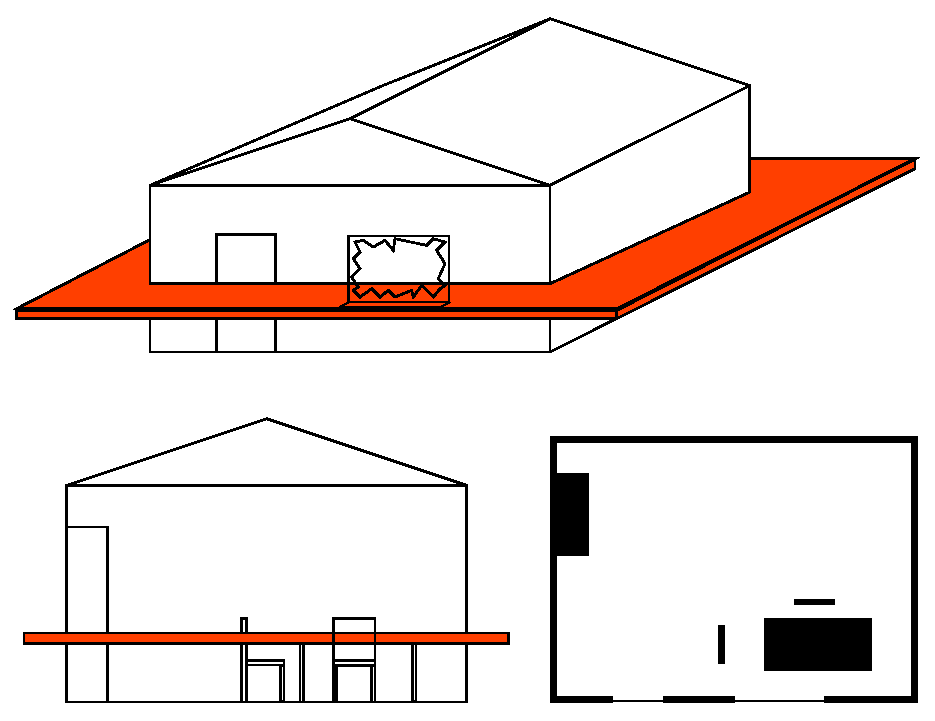
\includegraphics[clip=true,
    width=120mm]{evac_grid2.eps}}
  \caption{A 2D evacuation mesh.}\label{Fig_EvacGrid} 
\end{figure}
%

All evacuation meshes should have a name, \emph{i.e.}, a keyword \Timtt{ID}
should be given on the \Timtt{\&MESH} line.  The name of the mesh
should not be too long, max 26 characters.  Of course, the names of
different meshes can not be the same.  The \Timtt{ID} is used later to
specify the mesh, where some additional evacuation objects are placed.

Evacuation meshes should have only one cell in the $z$ direction,
i.e., they are two-dimensional horizontal meshes, see
Figure~\ref{Fig_EvacGrid}.  Choose \Timtt{IJK} and \Timtt{XB} so that
the $dx$ and $dy$ are nice round numbers, which will fit nicely to
your geometry.  You should give the positions of all evacuation
objects as multiples of $dx$ and $dy$.  This is not obligatory but one
makes less mistakes this way.  FDS+Evac does not move the evacuation
objects to the closest mesh points yet, this may change in later
versions of FDS+Evac.

Evacuation meshes, which are only used to calculate (additional) human
movement flow fields should have \Timtt{EVAC\_HUMANS=.FALSE.} or just
no \Timtt{EVAC\_HUMANS} keyword at all.  False is the default.  Note,
that these meshes should have exactly the same \Timtt{IJK} and
\Timtt{XB} definitions as the corresponding main evacuation meshes.
This is not checked by the program so the user should do the check.
 


\subsection{The \Timtt{TIME} Namelist Group}

\begin{description}
%
\item[\Timts{EVAC\_DT\_FLOWFIELD}] is the time step of the calculation
  of the evacuation flow fields.  These fields are calculated before
  the fire and evacuation calculation, \emph{i.e.}, simulation time
  has negative values. (Default is 0.01~s.)
%
\item[\Timts{EVAC\_DT\_STEADY\_STATE}] is the maximum time step of the
  human movement algorithm, this should not be too large, should not
  be larger than 0.1~s.  This parameter defines the minimum coupling
  frequency of different main evacuation meshes.  Coupling is faster
  if the time step of the fire calculation is shorter. (Default is
  0.05~s.)
%
\end{description}



\subsection{The \Timtt{SURF} Namelist Group}

One should always define a new surface type for the evacuation
calculation, which is used to construct the flow fields that guide the
humans to the doors (or to other targets), see
Figure~\ref{Fig_EvacFlowField} and the FDS+Evac Technical Reference
Guide for details.  The following line should be given on the input
file:
\begin{verbatim}
  &SURF ID = 'OUTFLOW', VEL = +0.000001, TAU_V=0.1 /  
\end{verbatim}
%
Note, that \Timtt{VEL} should be a really small number, otherwise one
might not get a nice 2D potential flow solution.




\subsection{The \Timtt{MISC} Namelist Group}

\begin{description}
%
\item[\Timts{EVAC\_SURF\_DEFAULT}] is the surface default for the
  evacuation meshes.  The default is \Timtt{INERT}.  You could specify
  some other solid material for the default surface material, but
  FDS+Evac uses only the color information.
%
\item[\Timts{EVAC\_PRESSURE\_ITERATIONS}] is the number of Poisson
  solver iterations at each human flow field time step.  If you human
  flow fields do not look nice, you might need to increase this.  Too
  large number makes the human flow field calculation to take too
  much CPU time.  (Default is 50.)
%
\item[\Timts{EVAC\_TIME\_ITERATIONS}] is the number of human flow
  field calculation time steps.  One should have a nice converged
  human flow field, so some iterations are needed.  Too large number
  means too long CPU time.  (Default is 50.)
%
\end{description}

The flow fields, which are used to guide humans out of the building or
to some other targets, are calculated before the actual fire and
evacuation simulation, \emph{i.e.}, flow field calculation has $t<0$.  The
product $t_\mathrm{flow} = \Timts{EVAC\_TIME\_ITERATIONS} \times
\Timts{EVAC\_DT\_FLOWFIELD}$ defines the duration of the evacuation
flow field calculation.  The fields should become 'steady-state'
during this time.  Note, that the ramp up time of the boundary
conditions \Timtt{TAU\_V=0.1} given on the \Timtt{\&SURF ID='OUTFLOW'}
line should be well below the duration of the flow field calculation
$t_\mathrm{flow}$.  Default $t_\mathrm{flow}$ is $50\times
0.01~\mathrm{s} = 0.5~\mathrm{s}$.




\subsection{The \Timtt{VENT} Namelist Group}

Because one needs to specify special \Timtt{VENT}s for the evacuation
calculation, the \Timtt{VENT} namelist group has an additional logical
item \Timtt{EVACUATION}.  If it is \Timtt{.TRUE.} then this
\Timtt{VENT} is omitted in the fire calculation.  The default value is
\Timtt{.FALSE.}  The keyword \Timtt{MESH\_ID} should also be given, if
the \Timtt{VENT} is not needed in all evacuation flow field
calculations on this floor.  Note, that an evacuation \Timtt{VENT}
without \Timtt{MESH\_ID} is put on every evacuation flow field on this
floor.  This means that it is better always to have the item
\Timtt{MESH\_ID} specified, if \Timtt{EVACUATION=.TRUE.} is given.
Note, that in FDS5 VENT must always be defined on a solid surface or
on the outer boundary of the computational domain.  Thus, the user may
need to place additional evacuation OBSTs behind the VENTs used to
generate the evacuation flow fields.



\subsection{The \Timtt{OBST} Namelist Group}

One may need to specify special \Timtt{OBST}s for the evacuation
calculation, which are not present in the fire calculation.  Thus, the
\Timtt{OBST} namelist group has an additional logical item
\Timtt{EVACUATION}.  If it is \Timtt{.TRUE.} then this \Timtt{OBST} is
omitted in the fire calculation.  If the evacuation flow fields need
different obstacles for different human flow fields, then the item
\Timtt{MESH\_ID} should be given for the evacuation obstacles.
Usually these additional evacuation obstacles are introduced at
places, where humans are not allowed to walk.



\subsection{The \Timtt{HOLE} Namelist Group}

This is similar to the \Timtt{OBST} namelist group.  Only difference
is that the \Timtt{HOLE} lines of the fire calculation should have a
keyword \Timtt{EVACUATION=.FALSE.} set and these lines should be
duplicated to the evacuation geometry having \Timtt{EVACUATION=.TRUE.}
set.  If the evacuation flow fields need different holes for different
fields, then the item \Timtt{MESH\_ID} should be given for the
evacuation calculation holes.  Holes are treated in the FDS input a
little bit different than the obstacles, \emph{i.e.}, first all obstacles are
read in and after this the holes are created.  This is true for all
meshes, so the evacuation meshes can mix holes and obstacles
incorrectly, if there are no \Timtt{EVACUATION=.FALSE.} on the fire
calculation holes.

If you have an ordinary FDS5 input file and want to use this as a
starting point of a FDS+Evac input file, you should add
\Timtt{EVACUATION=.FALSE.} keyword to every \Timtt{HOLE} line, which
you have in the FDS5 fire input.  After this, you should duplicate
these hole lines and change the kewyword \Timtt{EVACUATION} value to
.TRUE. if you want the same holes to appear correctly in the
evacuation geometry.


\subsection{The \Timtt{PERS} Namelist Group}

This namelist group is used to define human types.  There are five
default human types defined and they are 'Adult', 'Male', 'Female',
'Child', and 'Elderly', see Table~\ref{Table_DefaultHumans} for their
properties.
%
\begin{description}
%
\item[\Timts{DEFAULT\_PROPERTIES}] 'Adult', 'Male', 'Female', 'Child',
  or 'Elderly'.  If not given, default values are used, see the end of
  Sec.~\ref{Sec_MoveModel}.  Note, that these values are overridden if
  they are explicitly given in the \Timtt{PERS} namelist input line.
%
\end{description}

Properties like human diameter, walking speed, pre-evacuation time,
and force constants are given here.  Some of the values might be given
as distributions.  The distribution types are chosen by keywords
\Timts{DIAMETER\_DIST, VELOCITY\_DIST, TAU\_EVAC\_DIST,}
\Timts{DET\_EVAC\_DIST,} and \Timtt{PRE\_EVAC\_DIST,} where the
choices for the statistical distributions are listed on
Table~\ref{Table_Distributions}.  The most used ones are: 0) no
distribution, \Timtt{x\_MEAN} is used; 1) uniform distribution,
\Timtt{x\_LOW} and \Timtt{x\_HIGH} are used; 2) normal distribution,
\Timtt{x\_MEAN} is the mean, \Timtt{x\_PARA} is the std.dev.,
\Timtt{x\_LOW} and \Timtt{x\_HIGH} are the cut offs, \emph{i.e.}, the values
are within the interval (\Timtt{x\_LOW},\Timtt{x\_HIGH}).  If
\Timtt{x\_LOW} is not given $\Rightarrow$ \Timtt{x\_LOW=0.0}.  If
\Timtt{x\_HIGH} is not given, then \Timtt{x\_HIGH} is a 'very large'
number.  Above, \Timtt{x} refers to one of the strings \Timts{DIA},
\Timts{VEL}, \Timts{TAU}, \Timts{DET}, or \Timtt{PRE}.


\begin{description}
%
\item[\Timtt{DET\_MEAN,DET\_PARA,DET\_PARA2,DET\_LOW,DET\_HIGH}]
  detection time, parameters of the distribution.
%
\item[\Timtt{PRE\_MEAN,PRE\_PARA,PRE\_PARA2,PRE\_LOW,PRE\_HIGH}]
  reaction time, parameters of the distribution (is equal to
  pre-evacuation time if no detection time is given).
%
\item[\Timts{VEL\_MEAN,VEL\_PARA,VEL\_PARA2,VEL\_LOW,VEL\_HIGH}] The
  target walking speed $v_i^0$, parameters of the distribution, see
  Eq.~\ref{Eq_force} and Table~\ref{Table_DefaultHumans}.
%
\item[\Timts{DIA\_MEAN,DIA\_PARA,DIA\_PARA2,DIA\_LOW,DIA\_HIGH}]
  Diameter of human circle ($2R_d$), parameters of the distribution,
  see Table.~\ref{Table_DefaultHumans} and Fig.~\ref{Fig_HumanBody}.
%
\item[\Timts{TAU\_MEAN,TAU\_PARA,TAU\_PARA2,TAU\_LOW,TAU\_HIGH}]
  relaxation time $\tau_i$, parameters of the distribution, see
  Eq.~\ref{Eq_force}.
%
\item[\Timts{FCONST\_A,FCONST\_B,L\_NON\_SP}] Social force parameters
  $A_i$, $B_i$, $\lambda_i$, see Eq.~\ref{Eq_socialforce}.
%
\item[\Timts{C\_YOUNG,KAPPA}] Contact force parameters $k$ and
  $\kappa$, see Eq.~\ref{Eq_contactforce}.
%
\item[\Timts{D\_TORSO\_MEAN,D\_SHOULDER\_MEAN}] The mean diameters of
  the torso and shoulder circles, see Table.~\ref{Table_DefaultHumans} and
  Fig.~\ref{Fig_HumanBody}.  The variation of the diameters is
  determined by the variation of the human circle ($2R_d$).
%
\item[\Timts{TAU\_ROT}] relaxation time $\tau_i^z$ for the
  rotational equation of motion, see Eq.~\ref{Eq_motive_torque}.
%
\item[\Timts{M\_INERTIA}] moment of inertia $I_i^z$ for the rotational
  equation of motion, see Eq.~\ref{Eq_rotmotion}.
%
\item[\Timts{FAC\_A\_WALL}] $A_w$ for walls is \Timtt{FAC\_A\_WALL}$*A_i$.
%
\item[\Timts{FAC\_B\_WALL}] $B_w$ for walls is \Timtt{FAC\_B\_WALL}$*B_i$.
%
\item[\Timts{LAMBDA\_WALL}] $\lambda_w$ for walls.
%
\item[\Timts{FC\_DAMPING}] Damping coefficient $c_d$ of the radial
  contact force, see Eq.~\ref{Eq_contactforce}.
%
\item[\Timts{V\_ANGULAR}] Maximum target angular speed of a human
  $\omega_i^0$, see Eq.~\ref{Eq_motive_torque}.
%
\item[\Timts{NOISEME,NOISETH}] Gaussian noise, see
  Eqs.~\ref{Eq_motion} and \ref{Eq_rotmotion}.  These parameters
  determine both the noise in the translational equation and the noise
  in the rotational equation.
%
%\item[\Timts{I\_FRIC\_SW}] Friction force switch:\\
%  1: $\kappa (d_{ij} - r_{ij}) \Delta v_{ij}^{t} \mathbf{t}_{ij}$~~
%  Default value, \\ 
%  0: $\gamma \Delta v_{ij}^{t} \mathbf{t}_{ij}$
%
\item[\Timts{COLOR\_METHOD}] How humans are shown in Smokeview, see
  Table~\ref{Table_ColorMethod}.  Default value is -1.
%
\item[\Timts{NOT\_RANDOM}] If true, do not use random seed when
  generating the initial positions and characteristics of humans.
  Default is false.
%
\item[\Timts{DENS\_INIT}] If > 2.0, then humans are tried to put on
  the initial positions so that they can be touching.  The default is
  to leave some space between humans and very large human densities
  are not possible.  Note that FDS+Evac puts humans randomly in their
  initial positions and, thus, the initial density of humans can not
  be much larger than 2 humams per square meter. (Default is 0.0.)
%
\item[\Timts{TDET\_SMOKE\_DENS}] If > 0.0 then a human detects the
  fire when the smoke density ($mg/m^3$) is larger than the given
  value at the position of the human if the human has not yet detected
  the fire due to the detection time distribution.  Default is no
  detection by smoke.
%
\item[\Timts{FED\_DOOR\_CRIT}] This sets the amount of ``smoke'' which
  is used to decide if some door is considered to be ``smoke free'' in
  the door selection algorithm of FDS+Evac.  If > 0.0 then a door is
  considered to be smoke free, if the estimated FED value for this
  humans is less than the given value.  If < 0.0 then the absolute
  value is the visibility distance (m) which is used by the door
  selection algorithm to rank a door as smoke free (visibility $S =
  3/K$).  Default is 0.000001.
%
\end{description}

\noindent NOTE: \Timts{FAC\_x\_WALL, LAMBDA\_WALL, FC\_DAMPING,
  V\_ANGULAR, NOISExx, COLOR\_METHOD, NOT\_RANDOM} the last values
read from \Timtt{PERS} lines are used.  So, it is nice practice to
give these numbers just in one \Timtt{PERS} group or have same numbers
in every \Timtt{PERS} group.

\noindent WARNING: Change only the reaction and detection time
parameters, other parameters should have the default values and use
the pre-defined person types, unless you know what you are doing.

 
\subsection{The \Timtt{EVAC} Namelist Group}

Places humans in the evacuation meshes, \emph{i.e.}, the initial positions of
the humans.
%
\begin{description}
%
\item[\Timtt{ID}] ID string of the group of humans.
%
\item[\Timtt{XB}] where the humans are put, $z$ should belong to a
  main evac mesh.
%
\item[\Timtt{NUMBER\_INITIAL\_PERSONS}] how many persons are put in
  the area \Timtt{XB}.
%
\item[\Timts{ANGLE}] By default the orientation of humans is random,
  but by giving angle (0--360) one can specify the orientation of
  persons.  Angle 0 means that humans are facing towards +$x$.
%
\item[\Timts{QUANTITY}] Color of the human torso in Smokeview.  The
  colors which can be used are: black, yellow, blue, red, green,
  magenta, and cyan.  Note, that if a person is dead, it is colored as
  \Timtt{CYAN}.  Default is \Timtt{BLACK}.
%
\item[\Timtt{PERS\_ID}] From which person class the properties are
  generated (randomly).  If no \Timtt{PERS\_ID} is given, then the
  default values are used.
%
\item[\Timts{FLOW\_FIELD\_ID}] Flow field in the 'room/floor', which
  this person is initially following, \emph{i.e.}, specifies to which door a
  person tries to go if no known nor visible door is available.
%
\item[\Timts{KNOWN\_DOOR\_NAMES}] The ID strings of the known exit
  doors.
%
\item[\Timts{KNOWN\_DOOR\_PROBS}] The probabilities that the exit
  doors are known.  At the initialization phase the known doors for
  persons are drawn using these probabilities. Default values are
  equal to ones.
%
\item[\Timts{MESH\_ID}] If there are overlapping main evacuation
  meshes then this parameter could be used to specify the mesh where
  this EVAC line is applied.
%
\item[\Timts{OUTPUT\_SPEED}]  The movement speed of human is saved in
  the ouput file to be shown in Smokeview as a color bar.
%
\item[\Timts{OUTPUT\_FED}]  The FED index of human is saved in
  the ouput file to be shown in Smokeview as a color bar.
%
\item[\Timts{OUTPUT\_CONTACT\_FORCE}] The contact force acting on
  human circumference (N/m) is saved in the ouput file to be shown in
  Smokeview as a color bar.
%
\item[\Timts{OUTPUT\_TOTAL\_FORCE}] The total force (contact + social)
  acting on human circumference (N/m) is saved in the ouput file to be
  shown in Smokeview as a color bar.
%
\end{description}


\noindent NOTE: If no \Timtt{PERS\_ID} is given on \Timtt{EVAC} lines,
then the default values are used for the properties of persons.
These default values are given inside the code, and they might be
changing during the development of the code.  So, one should not use
the default values.


\subsection{The \Timtt{EVHO} Namelist Group}
%
\begin{description}
%
\item[\Timtt{ID}] ID string.
%
\item[\Timtt{XB}] where the humans are not put, $z$ should belong to a
  main evac mesh.
%
\item[\Timts{PERS\_ID}] This hole apply just for this person type,
  \emph{i.e.}, has effect only on those \Timtt{EVAC} lines, where
  \Timts{PERS\_ID} matches.
%
\item[\Timts{EVAC\_ID}] This hole apply just for on that \Timtt{EVAC}
  line.  If both \Timts{PERS\_ID} and \Timts{EVAC\_ID} are given, they
  are treated using the logical operator OR.
%
\item[\Timts{MESH\_ID}] If there are overlapping main evacuation
  meshes then this parameter could be used to specify the mesh where
  this EVHO line is applied.
%
%
\end{description}



\subsection{The \Timtt{EXIT} Namelist Group}

Defines an exit.  Note, that an 'outflow' vent is not automatically
created, so the user should give a separate \Timtt{VENT} line.  Exits
might be used just to count humans, then the keyword
\Timts{COUNT\_ONLY=.TRUE.} is used and, thus, these can be placed
anywhere inside the building.  Humans, which move through an exit
(\Timts{COUNT\_ONLY=.FALSE.}), are removed from the calculation, \emph{i.e.},
they are supposed to be gone outside of the building and be safe.

\begin{description}
%
\item[\Timtt{ID}] ID string of the exit. One can refer to this exit by
  its name.
%
\item[\Timtt{XB}] Co-ordinates, should be a line in the $(x,y)$ plane,
  the $z$ should belong to a main evacuation mesh.
%
\item[\Timtt{IOR}] Direction of the door, e.g., +1 humans are going
  $+x$ direction -2 humans are going $-y$ direction (direction means:
  room $\Rightarrow$ exit $\Rightarrow$ outside of the building)
%
\item[\Timts{COUNT\_ONLY}] If true, humans are not removed, they are
  just counted (default is false).  The CHID\_evac.csv file has a
  column for each \Timtt{EXIT} regardless if \Timts{COUNT\_ONLY} is
  true or false.
%
\item[\Timts{VENT\_FFIELD}] The ID string of the evacuation flow field
  behind this exit door.  The humans are guided to this exit door by
  the specified flow field.
%
\item[\Timts{FLOW\_FIELD\_ID}] Used, if this exit is a target for some
  other evacuation element and there are no known doors nor visible
  ones available.  If \Timts{FLOW\_FIELD\_ID} is not given, then the
  main evacuation mesh flow field is used.  WARNING: It is better to
  use a door or an entry instead of an exit if it is a target of some
  other evacuation element.
%
\item[\Timts{XYZ}] Co-ordinates, which are used in the exit door
  selection algorithm to decide if the exit is visible or not.
  Default is the mid-point of XB.
%
\item[\Timts{MESH\_ID}] If there are overlapping main evacuation
  meshes then this parameter could be used to specify the mesh where
  this EXIT line is applied.
%
\item[\Timts{COLOR\_INDEX}] Color index of the human torso in Smokeview
  if the \Timtt{COLOR\_METHOD}=4 on \Timtt{PERS} namelist.  The colors
  which can be used are: black (0), yellow(1), blue(2), red(3),
  green(4), magenta(5), and cyan(6).  Default is 0.
%
\item[\Timts{TIME\_OPEN}] The time (s) when this exit becomes usable.
  The default is that the exit is always usable.
%
\item[\Timts{TIME\_OPEN}] The time (s) when this exit becomes
  unusable.  The default is that the exit is always usable.
%
\end{description}




\subsection{The \Timtt{ENTR} Namelist Group}

Defines an entry.  An entry can enter humans to the calculation at a
constant frequency.  An entry with frequency zero can just be used as
an end point of a corridor (or some door).  This case corresponds to a
one way door, \emph{i.e.}, humans can only come out from this 'door'. 

\begin{description}
%
\item[\Timtt{ID}] ID string of the entry. One can refer to this entry
  by its name.
%
\item[\Timtt{IOR}] direction of the entry, e.g., +1 humans are
  entering towards $+x$ direction -2 humans are entering towards $-y$
  direction (direction means: somewhere $\Rightarrow$ entry
  $\Rightarrow$ room)
%
\item[\Timtt{MAX\_FLOW}] persons per second (actual flow may be
  smaller, if the area in front of the entry is crowded)
%
\item[\Timts{FLOW\_FIELD\_ID}] Flow field in the 'room/floor', which
  this person is following, \emph{i.e.}, specifies to which door a person
  tries to go if no known nor visible doors are available.  If not
  given, the flow field of the main evacuation mesh is used.
%
\item[\Timts{KNOWN\_DOOR\_NAMES}] The ID strings of the known exit
  doors.  This only apply to persons that are generated at this entry
  by the MAX\_FLOW, \emph{i.e.}, it does not apply to those persons who are
  transfered to this entry from somewhere else.
%
\item[\Timts{KNOWN\_DOOR\_PROBS}] The probabilities that the exit
  doors are known.  The known doors for the persons generated by this
  entry are drawn using these probabilities. Default values are equal
  to ones.
%
\item[\Timtt{XB}] coordinates, should be a line in the $(x,y)$ plane,
  the $z$ should be 'main evac mesh' $z$ coordinates.
%
\item[\Timts{QUANTITY}] color of the squares in Smokeview of the
  humans which are entered at a specific flow rate.  If the humans are
  coming to this entry form some other node, then their original color
  is used instead of \Timtt{QUANTITY}.  This is used if the
  COLOR\_METHOD=0 is specified on (some) PERS line.
%
\item[\Timtt{PERS\_ID}] the properties of humans are generated using
  these parameters, if they are not coming to this entry form some
  other node, \emph{i.e.}, they are 'new' humans.  If not given, default
  values are used.
%
\item[\Timts{MESH\_ID}] If there are overlapping main evacuation
  meshes then this parameter could be used to specify the mesh where
  this ENTR line is applied.
%
\end{description}



\subsection{The \Timtt{DOOR} Namelist Group}

Defines a door.  Similar to \Timtt{EXIT}, but the humans are not
removed from the calculation.  The humans are put to some other part
of the calculation (e.g., to a stairs, to a different 'room' etc.)

\begin{description}
%
\item[\Timtt{ID}] ID string of the door. One can refer to this door by
  its name.
%
\item[\Timtt{XB}] coordinates, should be a line in the $(x,y)$ plane,
  the $z$ should belong to a main evacuation mesh.
%
\item[\Timtt{IOR}] direction of the door, e.g., +1 humans are going
  $+x$ direction -2 humans are going $-y$ direction (direction means:
  room $\Rightarrow$ door $\Rightarrow$ some other place)
%
\item[\Timts{VENT\_FFIELD}] The ID string of the evacuation flow field
  behind this exit door.  The humans are guided to this exit door by
  the specified flow field.
%
\item[\Timts{FLOW\_FIELD\_ID}] Used, if this door is a target for some
  other evacuation element and there are no known doors nor visible
  ones available.  If no \Timtt{FLOW\_FIELD\_ID} is given, then the
  main evacuation mesh flow field of this floor is used.
%
\item[\Timts{EXIT\_SIGN}] If .TRUE. then this door is considered as an
  ``exit door'' in the door selection algorithm.  Humans can use this
  door even if it is not described as ``known door'', i.e., it can be
  classified as a ``visible, unknown door'' in the door selection
  algorithm. (Default is .FALSE.)
%
\item[\Timts{XYZ}] Co-ordinates, which are used in the exit door
  selection algorithm to decide if the door is visible or not.
  Default is the mid-point of XB.
%
\item[\Timts{KEEP\_XY}] saves the information on the position of the
  person relative to the width of the door, \emph{i.e.}, if the target of
  this door is DOOR or ENTR then human is placed according to this
  information.
%
\item[\Timtt{TO\_NODE}] Where humans are going, when going inside this
  door.  \Timtt{TO\_NODE} can be \Timtt{DOOR, EXIT, CORR,} or
  \Timtt{ENTR}.
%
\item[\Timts{MESH\_ID}] If there are overlapping main evacuation
  meshes then this parameter could be used to specify the mesh where
  this DOOR line is applied.
%
\item[\Timts{COLOR\_INDEX}] Color index of the human torso in Smokeview
  if the \Timtt{COLOR\_METHOD}=4 on \Timtt{PERS} namelist.  The colors
  which can be used are: black (0), yellow(1), blue(2), red(3),
  green(4), magenta(5), and cyan(6).  Default is 0.
%
\item[\Timts{TIME\_OPEN}] The time (s) when this door becomes usable.
  The default is that the door is always usable.
%
\item[\Timts{TIME\_OPEN}] The time (s) when this door becomes
  unusable.  The default is that the door is always usable.
%
\end{description}



\subsection{The \Timtt{CORR} Namelist Group}

Defines stairs (or a horizontal corridor).  One uses these to move
humans from one floor to the next one.  The corridor (actually stairs)
model is a really simple one.  One gives the length of the stairs and
reduces the movement speed.  One also gives the maximum number of
persons inside the corridor.  For now there is no relation between the
density and the movement speed (or human flow) inside the corridor.

\begin{description}
%
\item[\Timtt{ID}] ID string of the corridor. One can refer to this
  \Timtt{CORR} by its name.
%
\item[\Timtt{MAX\_HUMANS\_INSIDE}] how many humans fit inside the
  corridor.
%
\item[\Timtt{XB, XB1, XB2}] Used to specify the points, where the
  smoke and FED data is taken for this corridor/stair.  If only one
  value is used for the corridor/stair, give \Timtt{XB}.  If the
  values at the beginning and at the end of the corridor/stair is
  used, give both \Timtt{XB1} and \Timtt{XB2}, respectively.
%
\item[\Timtt{EFF\_LENGTH}] length of the corridor, movement time =
  \Timtt{EFF\_LENGTH}/\Timtt{FAC\_SPEED}$\times v_i^0$.
%
\item[\Timtt{FAC\_SPEED}] How much slower humans move in the corridor
  (e.g., stairs) compared to the (target) speed $v_i^0$ in floors.
%
\item[\Timtt{TO\_NODE}] Where humans are going, when leaving this
  corridor. To\_node can be \Timtt{DOOR, EXIT, CORR}, or \Timtt{ENTR}.
%
\end{description}
%
Note, that \Timtt{CORR} is usually used to define stairs between
floors: $\mathrm{Door_{2^{nd} ~floor}} ~ \rightarrow ~
\mathrm{Corr} ~ \rightarrow ~ \mathrm{Door_{1^{st} ~floor}}$.  Stairs
could also be constructed using the EVSS namelists correctly, but this
is not as straight forward as to use CORR constructions.



\subsection{The \Timtt{EVSS} Namelist Group}

Defines an incline (e.g., stairs or spectator stand) or an escalator.
The defined 'incline' could also be horizontal.  Then it specifies a
piece of the current floor at different vertical position than given
on the MESH line of the evacuation floor.  The $z$ co-ordinates of the
EVSS constructions are only used to plot the humans in 'correct'
positions when they are viewed by Smokeview.  The human movement
algorithm uses only the $x$ and $y$.

\begin{description}
%
%
\item[\Timtt{ID}] ID string of the incline.
%
\item[\Timtt{XB}] co-ordinates, should define a plane in the $(x,y)$
  plane, the $z$ should belong to a main evacuation mesh.
%
\item[\Timts{MESH\_ID}] If there are overlapping main evacuation
  meshes then this parameter could be used to specify the mesh where
  this EVSS line is applied.
%
\item[\Timtt{IOR}] direction of the incline, e.g., +1 means that the
  +$x$ edge of the EVSS plane is touching the main evacuation plane
  defined by the $z$ of XB.
%
\item[\Timtt{HEIGHT}] The height of the incline measured from the
  level of the main evacuation plane defined by the $z$ of XB. The
  other edge (opposite to the IOR edge) of the incline has $z =
  z_{\scriptscriptstyle XB} + \mathrm{height}$. HEIGTH can have a
  positive or a negative value.
%
\item[\Timts{HEIGHT0}] The height of the base line of the incline
  measured from the level of the main evacuation plane defined by the
  $z$ of XB. The IOR edge of the incline has $z =
  z_{\scriptscriptstyle XB} + \mathrm{height0}$. HEIGTH0 can have a
  positive or a negative value. If \Timts{HEIGHT0}=\Timts{HEIGHT} the
  EVSS defines a horisontal plane and IOR has no effect.
%
\item[\Timts{FAC\_V0\_UP}] The unimpeded speed of a human upwards the
  plane is $v = \mathit{FAC\_V0\_UP} \times v_0$.
%
\item[\Timts{FAC\_V0\_DOWN}] The unimpeded speed of a human downwards
  the plane is $v = \mathit{FAC\_V0\_DOWN} \times v_0$.
%
\item[\Timts{FAC\_V0\_HORI}] The unimpeded speed of a human
  horisontally along the plane is $v = \mathit{FAC\_V0\_HORI} \times
  v_0$.
%
\item[\Timts{ESC\_SPEED}] The speed of an escalator. One can use EVSS
  as a simple model of an escalator, humans are all moving with the
  velocity ESC\_SPEED along the escalator, \emph{i.e.}, they are not
  overtaking each others or walking on the escalator.
%
%
\end{description}
%

\clearpage



\section{Additional FDS+Evac Input Files}\label{Sec_InFiles}

The FDS+Evac calculation might have also other input files than the
\Timtt{CHID.fds} file.  These files are not needed but they may be
used to speed up the calculation and also to separate the fire and
evacuation parts of the calculation.

The file \Timtt{CHID\_evac.eff} contains the converged human flow
fields, which are calculated at the beginning of the FDS+Evac
calculation.  If this file exist and there are no fire meshes
(\Timtt{EVACUATION=.FALSE.}), it is read in.  Otherwise it is
(re)calculated and saved on the disk.  This file is useful if one is
doing many human egress calculations using exactly the same geometry
but with different human input, e.g., varying the number of humans,
the democraphics of humans, etc.  It is very useful when doing Monte
Carlo calculations in a quite complex buildings.  One do not need
every time to calculate the human flow fields and, thus, one is saving
some CPU seconds.

The file \Timtt{CHID\_evac.fed} contains the smoke and gas
concentration information from the FDS5 fire calculation.  This file
is tried to read in, if there are no 'fire' meshes
(\Timtt{EVACUATION=.FALSE.}) specified in the input.  If there is at
least one 'fire' mesh specified and also at least one main evacuation
mesh (\Timtt{EVAC\_HUMANS=.TRUE.} and \Timtt{EVACUATION=.TRUE.})
specified, then this file is (re)calculated and saved on the disk.

Note, that both files \Timtt{CHID\_evac.eff} and
\Timtt{CHID\_evac.fed} are assuming that the evacuation meshes and
geometry are exactly the same in the new calculation than was in the
one, which wrote the files.



\section{FDS+Evac: Output Files}\label{Sec_OutFiles}


FDS+Evac produces a file \Timtt{CHID\_evac.csv}, which has information
on the number of humans on the different floors and stairs at a given
time as well as the total number of humans inside the building.  The
file also list the number of humans gone through each exit and door.
The first column is the time and the second column is the number of
humans inside the whole building.  Then the number of humans in each
main evacuation meshes (``floors'') and in each corridor/stairs
(\Timtt{CORR} namelists) are given.  After these the number of humans
gone through various exits and doors are reported.  The last three
columns are printed only if the FED is used, \emph{i.e.}, the smoke and toxic
gas information is available.  The first of these columns reports the
number of dead humans, \emph{i.e.}, those whose FED values are larger than
unity.  The next column is the maximum value of FED among all humans,
dead or alive.  Note, that the FED value of the ``dead'' humans will
continue to build up as if they would be alive.  Finally, the last
column is the maximum FED value of the humans which are alive.

Human movement may be visualized by Smokeview, where 'Evacuation' is
shown on the Load/Save menu.  The humans are saved on '.prt5' files.
During the run of FDS+Evac lots of evacuation information is printed
on the standard error.  If you want to save this information, you
should redirect the standard error to some file.  Read your DOS or
Unix/Linux manual how to do this (\Timtt{2\&>1 > CHID.err}).

The file \Timtt{CHID\_evac.eff} contains the converged human flow
fields and the file \Timtt{CHID\_evac.fed} contains the smoke and gas
concentration information.  These might be used later, if more
evacuation calculations are done using same geometrical information,
e.g., if one is doing a Monte Carlo simulation of the egress scenario.

\clearpage


\section{Sample Input Files}\label{Sec_SampleFile}

Below two example inputs files of FDS+Evac are given.  These input
files are not representing any real building, they are just used to
show some of the keywords and parameters, which can be used in
FDS+Evac egress calculation.


\begin{figure}[!tb]
  \centerline{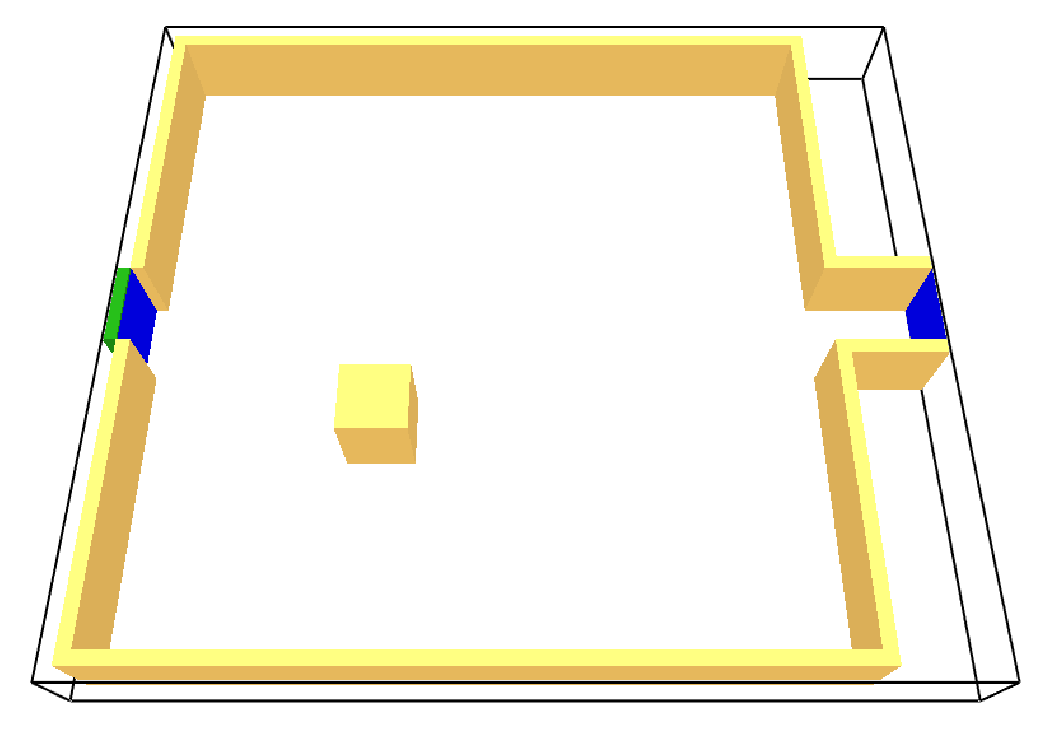
\includegraphics[clip=true,
    width=80mm]{evac_example1_EvacGeom.eps}~~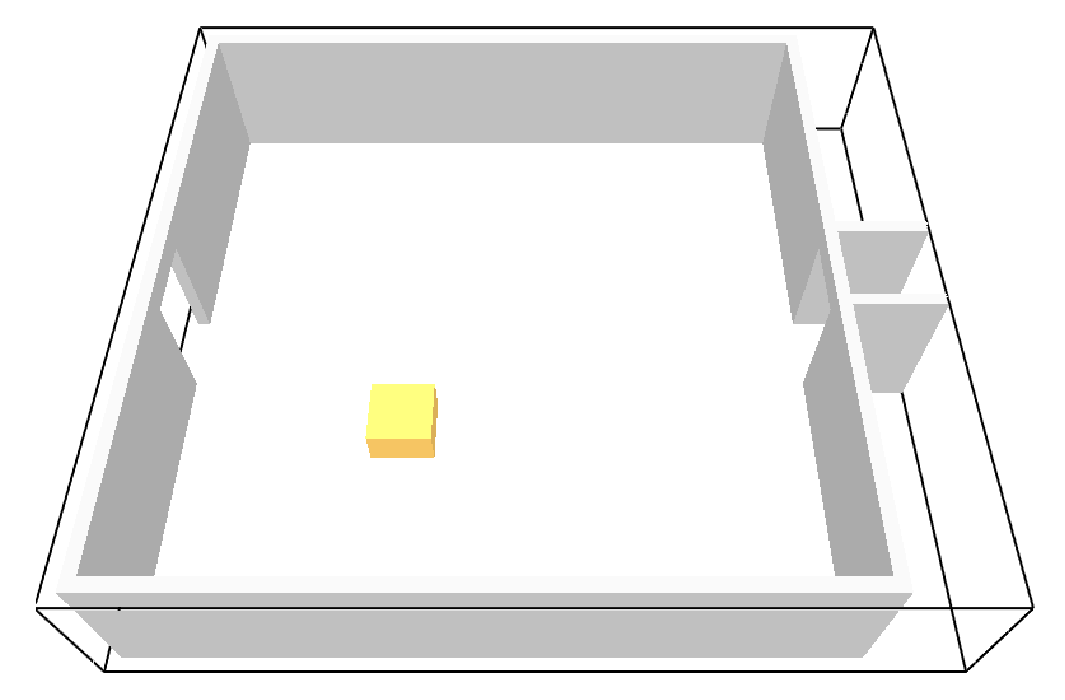
\includegraphics[clip=true,
    width=80mm]{evac_example1_FireGeom.eps}}
  \caption{Example 1: Evacuation and fire calculation
    geometries.}\label{Fig_Ex1EvacGeom}
\end{figure}

%\begin{figure}[!tb]
%  \centerline{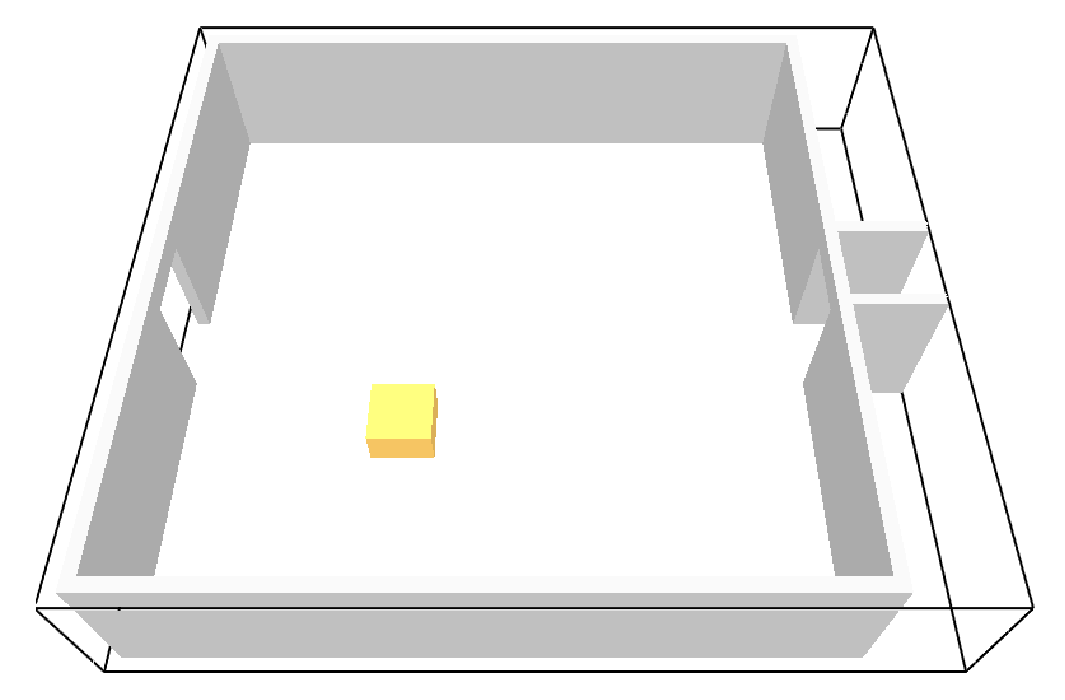
\includegraphics[clip=true,
%    width=120mm]{evac_example1_FireGeom.eps}}
%  \caption{.}\label{Fig_Ex1FireGeom}  
%\end{figure}

The first input file specifies a fire in a room with two doors, see
Fig.~\ref{Fig_Ex1EvacGeom}.  Humans are using both doors and they
select the door by using the exit door selection algorithm, thus, each
of the two doors needs its own evacuation flow field.  This means that
one needs to define the main evacuation mesh and two additional door
flow field meshes for this case besides the fire mesh.

\begin{verbatim}
&HEAD CHID='evac_example1', TITLE='Room Evacuation Test'  / 

 Fire mesh(es).
&MESH IJK=60,54,12, XB= -0.4,11.6, -0.4,10.4, 0.0,2.4 /

 One floor with 2 exit doors, thus, we need:
     one main evac mesh  (EVACUATION=.TRUE., EVAC_HUMANS=.TRUE.)
     two door flow meshes (EVACUATION=.TRUE., EVAC_HUMANS=.FALSE.)

 Main evacuation mesh for this floor. This mesh contains the humans.
 Evacuation meshes should all have an unique ID string defined.

&MESH IJK=60,54,1, XB= -0.4,11.6, -0.4,10.4, 0.4,1.6, EVAC_Z_OFFSET=1.0,
      EVACUATION=.TRUE., EVAC_HUMANS=.TRUE., ID='MainEvacGrid' /

 Additional door flow fields.
 Note: main evacuation mesh and the door flow meshes should have
 same XB and IJK.

&MESH IJK=60,54,1, XB= -0.4,11.6, -0.4,10.4, 0.4,1.6,
      EVACUATION=.TRUE., ID='LeftExitGrid' /
&MESH IJK=60,54,1, XB= -0.4,11.6, -0.4,10.4, 0.4,1.6, 
      EVACUATION=.TRUE., ID='RightExitGrid' /

&TIME TWFIN=200.0 / 

&MISC SURF_DEFAULT='WALL' / 

&DUMP NFRAMES=200,
      DT_PART=0.5,
      DT_HRR=1.0,
      DT_SLCF=1.0,
      DT_PL3D=10.0,
      DT_ISOF=10.0 /

&REAC ID         = 'POLYURETHANE'
      FYI        = 'C_6.3 H_7.1 N O_2.1, NFPA Handbook, Babrauskas'
      SOOT_YIELD = 0.10
      N          = 1.0
      C          = 6.3
      H          = 7.1
      O          = 2.1  /

&SURF ID='BURNER', HRRPUA=1000., PART_ID='smoke', COLOR='RASPBERRY' /

&MATL ID            = 'GYPSUM PLASTER'
      FYI           = 'Quintiere, Fire Behavior'
      CONDUCTIVITY  = 0.48
      SPECIFIC_HEAT = 0.84
      DENSITY       = 1440. /

&SURF ID             = 'WALL'
      RGB            = 200,200,200
      MATL_ID        = 'GYPSUM PLASTER'
      THICKNESS      = 0.012 /

&PART ID='smoke', MASSLESS=.TRUE., SAMPLING_FACTOR=1 /

 Ordinary fire calculation geometry input.
&OBST XB= -0.20, 0.00, -0.20, 10.20, 0.00, 2.40 /
&OBST XB= 10.00,10.20, -0.20, 10.20, 0.00, 2.40 /
&OBST XB= -0.20,10.20, -0.20,  0.00, 0.00, 2.40 /
&OBST XB= -0.20,10.20, 10.00, 10.20, 0.00, 2.40 /
&OBST XB= 10.00,11.60,  4.20,  4.40, 0.00, 2.40 /
&OBST XB= 10.00,11.60,  5.60,  5.80, 0.00, 2.40 /
&HOLE XB= -0.21, 0.01,  4.39,  5.61, 0.00, 2.00 /
&HOLE XB=  9.99,10.21,  4.39,  5.61, 0.00, 2.00 /

 The fire as a burner.
&OBST XB= 3.00, 4.00, 3.00, 4.00, 0.00, 0.60, SURF_ID='INERT' /
&VENT XB= 3.00, 4.00, 3.00, 4.00, 0.60, 0.60, SURF_ID='BURNER', 
      EVACUATION=.FALSE. /

 Note, that EVACUATION=.FALSE. should be given for 'MB' vents or
 otherwise these vent are introduce also to the evacuation geometry.
&VENT MB='YMIN',SURF_ID='OPEN', EVACUATION=.FALSE. / 
&VENT MB='YMAX',SURF_ID='OPEN', EVACUATION=.FALSE. / 

 Evacuation geometry input.

 Fire geometry holes should be duplicated, if they are also wanted
 to show up in the evacuation geometry.
&HOLE XB= -0.21, 0.01,  4.39,  5.61, 0.00, 2.00, EVACUATION=.TRUE./
&HOLE XB=  9.99,10.21,  4.39,  5.61, 0.00, 2.00, EVACUATION=.TRUE./

 A fan boundary condition is used to calculate the evacuation 
 flow fields.
&SURF ID = 'OUTFLOW', VEL = +0.00001, TAU_V=0.1 /

 Define the evacuation vents for the main evacuation mesh, there
 should be an evacuation vent at every place, where humans can
 go 'inside' some door, exit, etc object.
 
 This vent is not at an outer boundary of the domain nor at a solid
 object, thus, there should be an OBST behind it.
 Left Exit:
&VENT XB= -0.20,-0.20,  4.40,5.60, 0.40,1.60, SURF_ID='OUTFLOW', 
      MESH_ID='MainEvacGrid', EVACUATION=.TRUE., RGB=0,0,255 /
&OBST XB= -0.40,-0.20,  4.40,5.60, 0.40,1.60, SURF_ID='INERT', 
      EVACUATION=.TRUE., RGB=30,150,20 / 
 
This vent is at the outer boundary of the domain, i.e., it is
 on a solid object, thus, no need for an OBST behind it.
 Right Exit:
&VENT XB= 11.60,11.60,  4.40,5.60, 0.40,1.60, SURF_ID='OUTFLOW', 
      MESH_ID='MainEvacGrid', EVACUATION=.TRUE., RGB=0,0,255/

 An exit namelist defines an exit door which takes humans out of the
 calculation.
&EXIT ID='LeftExit', IOR=-1,
      FYI= 'Comment line',
      VENT_FFIELD='LeftExitGrid',
      COLOR_INDEX=2,
      XYZ= 0.20, 5.00, 1.50,
      XB= -0.20,-0.20,  4.40,5.60, 0.40,1.60 /
&VENT XB= -0.20,-0.20,  4.40,5.60, 0.40,1.60, SURF_ID='OUTFLOW', 
      MESH_ID='LeftExitGrid', EVACUATION=.TRUE./ Left Exit Fan

&EXIT ID='RightExit', IOR=+1,
      FYI= 'Comment line',
      VENT_FFIELD='RightExitGrid',
      COLOR_INDEX=3,
      XYZ= 9.80, 5.00, 1.50,
      XB= 11.60,11.60,  4.40,5.60, 0.40,1.60 /
&VENT XB= 11.60,11.60,  4.40,5.60, 0.40,1.60, SURF_ID='OUTFLOW', 
      MESH_ID='RightExitGrid', EVACUATION=.TRUE./ Right Exit Fan

 Next is just a counter.
&EXIT ID='RightCounter', IOR=+1,
      FYI= 'Comment line',
      COUNT_ONLY=.TRUE.,
      XB= 10.00,10.00,  4.40,5.60, 0.40,1.60 /

 Evacuation calculation, human properties
 Note: Parameters DENS_INIT and COLOR_METHOD affect all humans and
       the values read in from the last '&PERS' line where they 
       exits are used for all humans. 
&PERS ID='Adult',
      FYI='Male+Female diameter and velocity',
      DEFAULT_PROPERTIES='Adult',
      PRE_EVAC_DIST=1,
      PRE_MEAN=10.0,PRE_LOW=5.0,PRE_HIGH=15.0,
      DET_EVAC_DIST=1,
      DET_MEAN=10.0,DET_LOW=5.00,DET_HIGH=15.0,
      DENS_INIT=4.0
      OUTPUT_SPEED=.TRUE.,
      OUTPUT_FED=.TRUE.,
      COLOR_METHOD = 0 /

&PERS ID='Male',
      FYI='Male diameter and velocity',
      DEFAULT_PROPERTIES='Male',
      PRE_EVAC_DIST=1,
      PRE_MEAN=10.0,PRE_LOW=5.0,PRE_HIGH=15.0,
      DET_EVAC_DIST=1,
      DET_MEAN=10.0,DET_LOW=5.00,DET_HIGH=15.0 /

&PERS ID='Female',
      FYI='Female diameter and velocity',
      DEFAULT_PROPERTIES='Female',
      PRE_EVAC_DIST=1,
      PRE_MEAN=10.0,PRE_LOW=5.0,PRE_HIGH=15.0,
      DET_EVAC_DIST=1,
      DET_MEAN=10.0,DET_LOW=5.00,DET_HIGH=15.0 /

&PERS ID='Child',
      FYI='Child diameter and velocity',
      DEFAULT_PROPERTIES='Child',
      PRE_EVAC_DIST=1,
      PRE_MEAN=10.0,PRE_LOW=5.0,PRE_HIGH=15.0,
      DET_EVAC_DIST=1,
      DET_MEAN=10.0,DET_LOW=5.00,DET_HIGH=15.0 /

&PERS ID='Elderly',
      FYI='Elderly diameter and velocity',
      DEFAULT_PROPERTIES='Elderly',
      PRE_EVAC_DIST=1,
      PRE_MEAN=10.0,PRE_LOW=5.0,PRE_HIGH=15.0,
      DET_EVAC_DIST=1,
      DET_MEAN=10.0,DET_LOW=5.00,DET_HIGH=15.0 /

 Initial positions of the humans

 These humans will go to the left exit, if it is not blocked by smoke.
&EVAC ID = 'HumanLeftDoorKnown', 
      NUMBER_INITIAL_PERSONS = 25,
      XB = 1.0,9.0,  1.0,9.0, 0.4,1.6
      QUANTITY = 'BLUE',
      KNOWN_DOOR_NAMES = 'LeftExit',
      KNOWN_DOOR_PROBS = 1.0,
      PERS_ID = 'Male' / 

 These humans will go to the right exit, if it is not blocked by smoke.
&EVAC ID = 'HumanRightDoorKnown', 
      NUMBER_INITIAL_PERSONS = 25,
      XB = 1.0,9.0,  1.0,9.0, 0.4,1.6
      QUANTITY = 'RED',
      KNOWN_DOOR_NAMES = 'RightExit',
      KNOWN_DOOR_PROBS = 1.0,
      PERS_ID = 'Female' / 

 These humans know both doors so they will use the nearest visible
 known door which is not blocked by smoke.
&EVAC ID = 'HumanBothDoorsKnown', 
      NUMBER_INITIAL_PERSONS = 25,
      XB = 1.0,9.0,  1.0,9.0, 0.4,1.6
      QUANTITY = 'GREEN',
      KNOWN_DOOR_NAMES = 'LeftExit','RightExit',
      KNOWN_DOOR_PROBS = 1.0,1.0,
      PERS_ID = 'Child' / 

 These humans do not have a known door and they will try to go to the
 nearest visible exit door. 
&EVAC ID = 'HumanNoDoorKnown', 
      NUMBER_INITIAL_PERSONS = 25,
      XB = 1.0,9.0,  1.0,9.0, 0.4,1.6
      QUANTITY = 'BLACK',
      PERS_ID = 'Adult' / 

 An evacuation hole, e.g., do not put humans on top of the fire.
&EVHO ID = 'Evho_Fire',
      FYI = 'Do not put humans close to the fire',
      XB = 2.0,5.0, 2.0,5.0, 0.4,1.6 /

 Fire calculation output.
&BNDF QUANTITY='WALL_TEMPERATURE' / 
&SLCF PBX=2.40, QUANTITY='TEMPERATURE' /

 Evacuation output used to plot the evacuation flow fields.
&SLCF PBZ = 1.500, QUANTITY = 'VELOCITY', VECTOR = .TRUE. / 

&TAIL /

\end{verbatim}

The second input file specifies a two-floor building, see
Fig.~\ref{Fig_Ex2EvacGeom}, each floor consisting of one human
movement area, \emph{i.e.}, only one main evacuation mesh per floor is
needed.  There is a fire in downstairs and the smoke is going to the
second floor by an opening at the ceiling.  The second floor is
connected to the first floor in the egress calculation, \emph{i.e.},
the second floor humans are transfered to the first floor by the
combination of doors and stairs.  The second floor has two exit doors,
one leading to the stairs going to the first floor (the right exit)
and one leading to the stairs leading directly to outside of the
building (the left exit).  The first floor has two exit doors.

\begin{figure}[!tb]
  \centerline{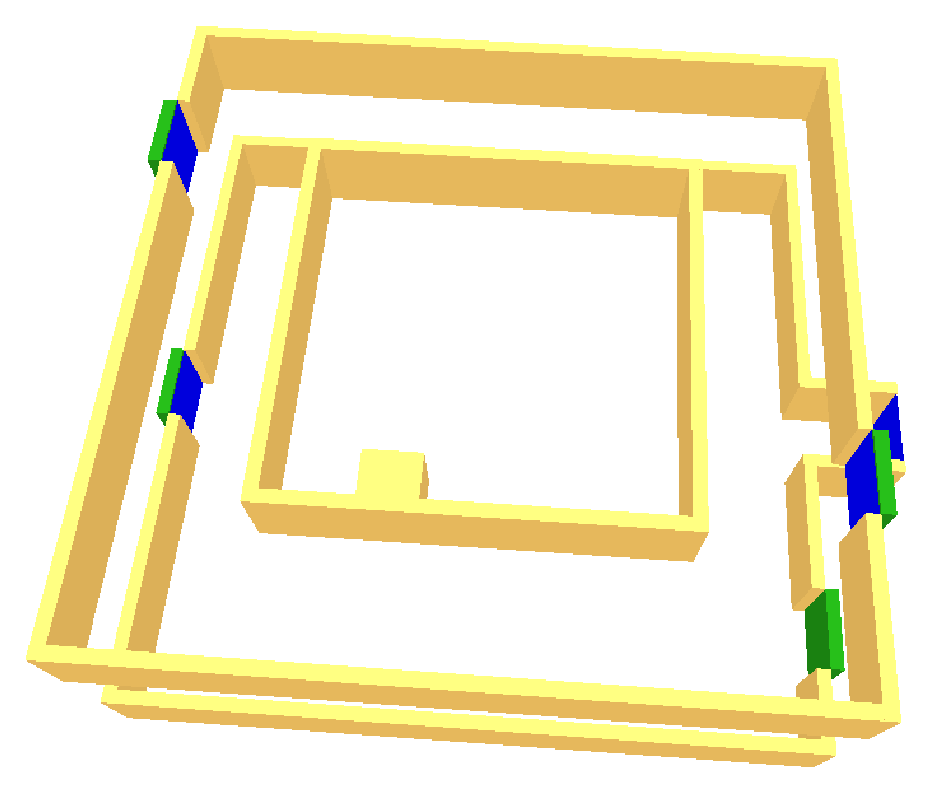
\includegraphics[clip=true,
    width=120mm]{evac_example2_EvacGeom.eps}}
  \caption{Example 2: Evacuation calculation
    geometry.}\label{Fig_Ex2EvacGeom}
\end{figure}


\begin{verbatim}

&HEAD CHID='evac_example2', TITLE='2 Floor Evacuation Test'  / 

 Fire mesh(es).
&MESH IJK=54,50,25, XB= -0.2,10.6,  0.0,10.0, 0.0,5.0 /

 Main evacuation meshes for the floors. These meshes contains the
 humans. Evacuation meshes should all have an unique ID string 
 defined.

&MESH IJK=60,54,1, XB= -0.4,11.6, -0.4,10.4, 0.4,1.6, EVAC_Z_OFFSET=1.0,
      EVACUATION=.TRUE., EVAC_HUMANS=.TRUE., ID='MainEvacGrid' /
&MESH IJK=54,54,1, XB= -0.4,10.4, -0.4,10.4, 3.0,4.2, EVAC_Z_OFFSET=1.0,
      EVACUATION=.TRUE., EVAC_HUMANS=.TRUE., ID='MainEvacGrid2' /

 Additional door flow fields.
 Note: main evacuation grid and the door flow grids should have
 same XB and IJK.

&MESH IJK=60,54,1, XB= -0.4,11.6, -0.4,10.4, 0.4,1.6,
      EVACUATION=.TRUE., ID='LeftExitGrid' / Left, 1st floor
&MESH IJK=60,54,1, XB= -0.4,11.6, -0.4,10.4, 0.4,1.6, 
      EVACUATION=.TRUE., ID='RightExitGrid' / Right, 1st floor

&MESH IJK=54,54,1, XB= -0.4,10.4, -0.4,10.4, 3.0,4.2,
      EVACUATION=.TRUE., ID='LeftDoorGrid2' / Left, 2nd floor
&MESH IJK=54,54,1, XB= -0.4,10.4, -0.4,10.4, 3.0,4.2, 
      EVACUATION=.TRUE., ID='RightDoorGrid2' / Right, 2nd floor

&TIME TWFIN=200.0 / 

&MISC SURF_DEFAULT='WALL' / 

&DUMP NFRAMES=200,
      DT_PART=0.5,
      DT_HRR=1.0,
      DT_SLCF=1.0,
      DT_PL3D=10.0,
      DT_ISOF=10.0 /

&REAC ID         = 'POLYURETHANE'
      FYI        = 'C_6.3 H_7.1 N O_2.1, NFPA Handbook, Babrauskas'
      SOOT_YIELD = 0.10
      N          = 1.0
      C          = 6.3
      H          = 7.1
      O          = 2.1  /

&SURF ID='BURNER', HRRPUA=1000., PART_ID='smoke', COLOR='RASPBERRY' /

&MATL ID            = 'GYPSUM PLASTER'
      FYI           = 'Quintiere, Fire Behavior'
      CONDUCTIVITY  = 0.48
      SPECIFIC_HEAT = 0.84
      DENSITY       = 1440. /

&SURF ID             = 'WALL'
      RGB            = 200,200,200
      MATL_ID        = 'GYPSUM PLASTER'
      THICKNESS      = 0.012 /

&PART ID='smoke', MASSLESS=.TRUE., SAMPLING_FACTOR=1 /

 Ordinary fire calculation geometry input.
&OBST XB= -0.20,10.20, -0.20, 10.20, 2.40, 2.60 / floor
&HOLE XB=  2.20, 7.80,  2.20,  7.80, 2.39, 2.61 / floor hole
&OBST XB=  2.00, 8.00,  2.00,  2.20, 2.60, 3.60 / balustrade
&OBST XB=  2.00, 8.00,  7.80,  8.00, 2.60, 3.60 / balustrade
&OBST XB=  2.00, 2.20,  2.00,  8.00, 2.60, 3.60 / balustrade
&OBST XB=  7.80, 8.00,  2.00,  8.00, 2.60, 3.60 / balustrade
&OBST XB= 10.20,11.60,  4.20,  5.80, 2.40, 2.60 / floor

&OBST XB= -0.20, 0.00, -0.20, 10.20, 0.00, 5.00 /
&OBST XB= 10.00,10.20, -0.20, 10.20, 0.00, 5.00 /
&OBST XB= -0.20,10.20, -0.20,  0.00, 0.00, 5.00 /
&OBST XB= -0.20,10.20, 10.00, 10.20, 0.00, 5.00 /
&OBST XB= 10.00,11.60,  4.20,  4.40, 0.00, 2.40 / Right Corridor Wall
&OBST XB= 10.00,11.60,  5.60,  5.80, 0.00, 2.40 / Right Corridor Wall
&HOLE XB= -0.21, 0.01,  4.39,  5.61, 0.00, 2.00 / Left Door
&HOLE XB=  9.99,10.21,  4.39,  5.61, 0.00, 2.00 / Right Door Hole

 The fire as an burner.
&OBST XB= 3.00, 4.00, 3.00, 4.00, 0.00, 0.60, SURF_ID='INERT' /
&VENT XB= 3.00, 4.00, 3.00, 4.00, 0.60, 0.60, SURF_ID='BURNER', 
      EVACUATION=.FALSE. /

 Note, that EVACUATION=.FALSE. should be given for 'MB' vents or
 otherwise these vent are introduce also to the evacuation geometry.
&VENT MB='YMIN',SURF_ID='OPEN', EVACUATION=.FALSE. / 
&VENT MB='YMAX',SURF_ID='OPEN', EVACUATION=.FALSE. / 

 Evacuation geometry input.

 Fire geometry holes should be duplicated, if they are also wanted
 to show up in the evacuation geometry.
&HOLE XB= -0.21, 0.01,  4.39,  5.61, 0.00, 2.00, EVACUATION=.TRUE./
&HOLE XB=  9.99,10.21,  4.39,  5.61, 0.00, 2.00, EVACUATION=.TRUE./

&HOLE XB= -0.21, 0.01,  7.39,  8.61, 2.60, 4.60, EVACUATION=.TRUE. /
&HOLE XB=  9.99,10.21,  2.39,  3.61, 2.60, 4.60, EVACUATION=.TRUE. /

 A fan boundary condition is used to calculate the evacuation
 flow fields.
&SURF ID = 'OUTFLOW', VEL = +0.00001, TAU_V=0.1 /

 Define the evacuation vents for the main evacuation meshes, there
 should be an evacuation vent at every place, where humans can
 go 'inside' some door, exit, etc object.

 This vent is not at an outer boundary of the domain nor at a solid
 object, thus, there should be an OBST behind it.
 Left Exit, 1st Floor:
&VENT XB= -0.20,-0.20,  4.40,5.60, 0.40,1.60, SURF_ID='OUTFLOW', 
      MESH_ID='MainEvacGrid', EVACUATION=.TRUE., RGB=0,0,255 /
&OBST XB= -0.40,-0.20,  4.40,5.60, 0.40,1.60, 
      EVACUATION=.TRUE., RGB=30,150,20 / 

 This vent is at the outer boundary of the domain, i.e., it is
 on a solid object, thus, no need for an OBST behind it.
 Right Exit, 1st Floor:
&VENT XB= 11.60,11.60,  4.40,5.60, 0.40,1.60, SURF_ID='OUTFLOW', 
      MESH_ID='MainEvacGrid', EVACUATION=.TRUE., RGB=0,0,255 /

 This vent is not at an outer boundary of the domain nor at a solid
 object, thus, there should be an OBST behind it.
 Right Exit, 2nd Floor:
&VENT XB= 10.20,10.20,  2.40,3.60, 3.0,4.2, SURF_ID='OUTFLOW', 
      MESH_ID='MainEvacGrid2', EVACUATION=.TRUE., RGB=0,0,255 /
&OBST XB= 10.20,10.40,  2.40,3.60, 3.0,4.2, 
      EVACUATION=.TRUE., RGB=30,150,20 / Right Door, 2nd

 This vent is not at an outer boundary of the domain nor at a solid
 object, thus, there should be an OBST behind it.
 Left Exit, 2nd Floor:
&VENT XB= -0.20,-0.20,  7.40,8.60, 3.0,4.2, SURF_ID='OUTFLOW', 
      MESH_ID='MainEvacGrid2', EVACUATION=.TRUE., RGB=0,0,255 /
&OBST XB= -0.40,-0.20,  7.40,8.60, 3.0,4.2, 
      EVACUATION=.TRUE., RGB=30,150,20 / Left Door, 2nd

 An exit namelist defines an exit door which takes humans out
 of the calculation.
&EXIT ID='LeftExit', IOR=-1,
      FYI= 'Comment line',
      VENT_FFIELD='LeftExitGrid',
      COLOR_INDEX=2,
      XYZ= 0.20, 5.00, 1.50,
      XB= -0.20,-0.20,  4.40,5.60, 0.40,1.60 /
&VENT XB= -0.20,-0.20,  4.40,5.60, 0.40,1.60, SURF_ID='OUTFLOW', 
      MESH_ID='LeftExitGrid', EVACUATION=.TRUE./ Left Exit Fan

&EXIT ID='RightExit', IOR=+1,
      FYI= 'Comment line',
      VENT_FFIELD='RightExitGrid',
      COLOR_INDEX=3,
      XYZ= 9.80, 5.00, 1.50,
      XB= 11.60,11.60,  4.40,5.60, 0.40,1.60 /
&VENT XB= 11.60,11.60,  4.40,5.60, 0.40,1.60, SURF_ID='OUTFLOW', 
      MESH_ID='RightExitGrid', EVACUATION=.TRUE./ Right Exit Fan

 Next is just a counter.
&EXIT ID='RightCounter', IOR=+1,
      FYI= 'Comment line',
      COUNT_ONLY=.TRUE.,
      XB= 10.00,10.00,  4.40,5.60, 0.40,1.60 /

 Second floor doors etc.

 This is a combination of a door leading to a stairs, which is
 leading directly to outside of the building: 
 DOOR ==> CORR ==> EXIT combination.
&DOOR ID='LeftDoor2nd', IOR=-1,
      FYI= 'Comment line',
      VENT_FFIELD='LeftDoorGrid2',
      TO_NODE= 'LeftCorr'
      COLOR_INDEX=4,
      EXIT_SIGN=.TRUE.,
      XYZ= 0.0, 8.00, 3.6,
      XB= -0.20,-0.20,  7.40,8.60, 3.0,4.2 /
&VENT XB= -0.20,-0.20,  7.40,8.60, 3.0,4.2 SURF_ID='OUTFLOW', 
      MESH_ID='LeftDoorGrid2', EVACUATION=.TRUE./ Left Door Fan, 2nd
&CORR ID='LeftCorr',
      FYI='Comments',
      MAX_HUMANS_INSIDE=20,
      EFF_LENGTH= 8.5,
      FAC_SPEED=0.7,
      TO_NODE='LeftCorrExit' /
&EXIT ID='LeftCorrExit',
      FYI='A dummy exit, the end point to a corridor object',
      IOR=-1,
      XB= -0.40,-0.40,  7.40,8.60, 0.40,1.60 /

 This is a combination of a door leading to a stairs, which is
 leading to the first floor: DOOR ==> CORR ==> ENTR combination.
&DOOR ID='RightDoor2nd', IOR=+1,
      FYI= 'Comment line',
      VENT_FFIELD='RightDoorGrid2',
      TO_NODE= 'RightCorr'
      COLOR_INDEX=5,
      EXIT_SIGN=.TRUE.,
      XYZ=10.0, 3.00, 3.6,
      XB= 10.20,10.20,  2.40,3.60, 3.0,4.2 /
&VENT XB= 10.20,10.20,  2.40,3.60, 3.0,4.2, SURF_ID='OUTFLOW', 
      MESH_ID='RightDoorGrid2', EVACUATION=.TRUE./ 
&CORR ID='RightCorr',
      FYI='Comments',
      MAX_HUMANS_INSIDE=20,
      EFF_LENGTH= 8.5,
      FAC_SPEED=0.7,
      TO_NODE='RightEntry' /
&ENTR ID='RightEntry',
      FYI='Comments',
      IOR=-1,
      XB=10.20,10.20,  1.00,2.20,  0.40,1.60 /
&HOLE XB= 9.99,10.20,  1.00,2.20,  0.40,1.60, 
      EVACUATION=.TRUE., RGB=30,150,20 / 1st Floor Entry
&OBST XB=10.20,10.40,  1.00,2.20,  0.40,1.60, 
      EVACUATION=.TRUE., RGB=30,150,20 / 1st Floor Entry

 Evacuation calculation, human properties
 Note: Parameters DENS_INIT and COLOR_METHOD affect all humans and
       the values read in from the last '&PERS' line where they 
       exits are used for all humans. 
&PERS ID='Adult',
      FYI='Male+Female diameter and velocity',
      DEFAULT_PROPERTIES='Adult',
      PRE_EVAC_DIST=1,
      PRE_MEAN=10.0,PRE_LOW=5.0,PRE_HIGH=15.0,
      DET_EVAC_DIST=1,
      DET_MEAN=10.0,DET_LOW=5.00,DET_HIGH=15.0,
      DENS_INIT= 4.0,
      OUTPUT_SPEED=.TRUE.,
      OUTPUT_FED=.TRUE.,
      COLOR_METHOD = 0 /

&PERS ID='Male',
      FYI='Male diameter and velocity',
      DEFAULT_PROPERTIES='Male',
      PRE_EVAC_DIST=1,
      PRE_MEAN=10.0,PRE_LOW=5.0,PRE_HIGH=15.0,
      DET_EVAC_DIST=1,
      DET_MEAN=10.0,DET_LOW=5.00,DET_HIGH=15.0 /

&PERS ID='Female',
      FYI='Female diameter and velocity',
      DEFAULT_PROPERTIES='Female',
      PRE_EVAC_DIST=1,
      PRE_MEAN=10.0,PRE_LOW=5.0,PRE_HIGH=15.0,
      DET_EVAC_DIST=1,
      DET_MEAN=10.0,DET_LOW=5.00,DET_HIGH=15.0 /

&PERS ID='Child',
      FYI='Child diameter and velocity',
      DEFAULT_PROPERTIES='Child',
      PRE_EVAC_DIST=1,
      PRE_MEAN=10.0,PRE_LOW=5.0,PRE_HIGH=15.0,
      DET_EVAC_DIST=1,
      DET_MEAN=10.0,DET_LOW=5.00,DET_HIGH=15.0 /

&PERS ID='Elderly',
      FYI='Elderly diameter and velocity',
      DEFAULT_PROPERTIES='Elderly',
      PRE_EVAC_DIST=1,
      PRE_MEAN=10.0,PRE_LOW=5.0,PRE_HIGH=15.0,
      DET_EVAC_DIST=1,
      DET_MEAN=10.0,DET_LOW=5.00,DET_HIGH=15.0 /

 Initial positions of the humans

 1st Floor:
 These humans will go to the left exit, if it is not blocked by smoke.
&EVAC ID = 'HumanLeftDoorKnown', 
      NUMBER_INITIAL_PERSONS = 25,
      XB = 1.0,9.0,  1.0,9.0, 0.4,1.6
      QUANTITY = 'BLUE',
      KNOWN_DOOR_NAMES = 'LeftExit',
      KNOWN_DOOR_PROBS = 1.0,
      PERS_ID = 'Male' / 

 These humans will go to the right exit, if it is not blocked by smoke.
&EVAC ID = 'HumanRightDoorKnown', 
      NUMBER_INITIAL_PERSONS = 25,
      XB = 1.0,9.0,  1.0,9.0, 0.4,1.6
      QUANTITY = 'RED',
      KNOWN_DOOR_NAMES = 'RightExit',
      KNOWN_DOOR_PROBS = 1.0,
      PERS_ID = 'Female' / 

 These humans know both doors so they will use the nearest visible
 known door which is not blocked by smoke.
&EVAC ID = 'HumanBothDoorsKnown', 
      NUMBER_INITIAL_PERSONS = 25,
      XB = 1.0,9.0,  1.0,9.0, 0.4,1.6
      QUANTITY = 'GREEN',
      KNOWN_DOOR_NAMES = 'LeftExit','RightExit',
      KNOWN_DOOR_PROBS = 1.0,1.0,
      PERS_ID = 'Child' / 

 These humans do not have a known door and they will try to go to
 the nearest visible exit door. 
&EVAC ID = 'HumanNoDoorKnown', 
      NUMBER_INITIAL_PERSONS = 25,
      XB = 1.0,9.0,  1.0,9.0, 0.4,1.6
      QUANTITY = 'BLACK',
      PERS_ID = 'Adult' / 

 2nd Floor:
 All of these humans know the right door on the 2nd floor and the
 right exit on the first floor. On the average, only 50 \% know
 the left door on the second floor and none knows the left exit
 on the first floor.
&EVAC ID = 'Human2ndFloor', 
      NUMBER_INITIAL_PERSONS = 50,
      XB = 0.5,9.5,  0.5,9.5, 3.0,4.2
      QUANTITY = 'MAGENTA',
      KNOWN_DOOR_NAMES = 'LeftDoor2nd','RightDoor2nd','RightExit',
      KNOWN_DOOR_PROBS = 0.5,1.0,1.0,
      PERS_ID = 'Adult' / 

 An evacuation hole, e.g., do not put humans on top of the fire.
&EVHO ID = 'Evho_Fire',
      FYI = 'Do not put humans close to the fire',
      XB = 2.0,5.0, 2.0,5.0, 0.4,1.6 /

 An evacuation hole, e.g., do not put humans on top of the opening
 in the ceiling.
&EVHO ID = 'Evho_2ndFloor',
      FYI = 'atrium space',
      XB = 2.0,8.0, 2.0,8.0, 3.0,4.2 /

 Fire calculation output.
&BNDF QUANTITY='WALL_TEMPERATURE' / 
&SLCF PBX=2.40, QUANTITY='TEMPERATURE' /

 Evacuation output used to plot the evacuation flow fields.
&SLCF PBZ = 1.000, QUANTITY = 'VELOCITY', VECTOR = .TRUE. / 
&SLCF PBZ = 3.600, QUANTITY = 'VELOCITY', VECTOR = .TRUE. / 

&TAIL /

\end{verbatim}

\newpage

\section{Conclusion}\label{Sec_Conclusions}

The FDS+Evac is under construction.  The next things to be implemented
are:
%
\begin{itemize}
%
\item Merging flows in corridors and stairs.
%
\item A more realistic \Timtt{CORR} object: Record the position of
  each human inside the corridor/stairs and use the equations of
  motion to model the movement in the corridor/stairs.
%
\item More pre-defined human classes, especially those refered in the
  IMO circular~\cite{IMO02}.
%
\item Elevators.
%
\item More intelligence in the exit door selection algorithm, e.g.,
  estimated queueing time due to the other humans heading towards the
  same exit door.
%
\item Social interactions like herding etc.
%
\item Sreading of the information: human to human communication.
%
\item Some support to the parallel version of the FDS5: The fire
  related information (the CHID\_evac.fed file) should be saved when
  doing parallel calculation.
%
\item Easier generation of the input file.
%
\end{itemize}
%

The present status of the FDS+Evac is:
%
\begin{itemize}
%
\item Smoke vs walking speed correlations are included.
%
\item Fractional Effective Dose is calculated and used to
  'incapacitate' humans.
%
\item Smoke density can be used to trigger human movement.
%
\item Simple exit door selection algorithm is implemented.
%
\item Inclines, stairs, escalators can be modelled explicitely by
  using the equations of motion for each person.
%
\item Simple stair algorithm without merging flows. If there are
  merging flows in staris then these should be modelled explicitely,
  which means some additional work to construct the input file.
%
\item The flows through doors, stairs and corridors are reproduced
  nicely by the underlaying dynamics.
%
\item Congestion can be studied.
%
\item The effect of the many input parameters of the human movement
  model are understood well and their effect on the human flows is
  known.
%
\end{itemize}
%

\noindent The shortcomings of FDS+Evac are:
%
\begin{itemize}
%
\item Geometry and the calculational mesh, \emph{i.e.}, rectanglular objects,
  whose edges are along the $x$ and $y$, are the main elements used to
  construct the geometry, including inclines and stairs.
%
\item Merging flows in stairs are not easy to model.
%
\item No elevators.
%
\item Evacuation calculations can only be done by the serial version
  of the FDS5 executable.
%
\item Visualization of the evacuation objects, like exits, door, etc.,
  on the Smokeview window.
%
\item The user input is not easy to give, \emph{i.e.}, no support for
  importing CAD drawings etc.
%
\end{itemize}
%

Users should notice that the evacuation part of FDS5 is under
development, and the features and user input may change in the future.

\clearpage

\addcontentsline{toc}{section}{References}
%\renewcommand{\bibname}{References}
\begin{thebibliography}{99}
%
%
\bibitem{Korhonen05} Korhonen, T., Hostikka, S., and Keski-Rahkonen,
  O., ``A Proposal for the Goals and New Techniques of Modelling
  Pedestrian Evacuation in Fires,'' Proceedings of the 8th
  International Symposium on Fire Safety Science, International
  Association for Fire Safety Science, pp.~557-567 (2005).
%
\bibitem{Korhonen07a} Korhonen, T., Hostikka, S., Heli\"ovaara, S.,
  Ehtamo, H., Matikainen, K., ``Integration of an Agent Based
  Evacuation Simulation and the State-of-the-Art Fire Simulation,''
  Proceedings of the 7th Asia-Oceania Symposium on Fire Science \&
  Technology, 20-22 September, 2007, Hong Kong, (in print).
%
\bibitem{Korhonen07b} Korhonen, T., Hostikka, S., Heli\"ovaara, S.,
  Ehtamo, H., Matikainen, K., ``FDS+Evac: Evacuation Module for Fire
  Dynamics Simulator,'' Proceedings of the Interflam2007: 11th
  International Conference on Fire Science and Engineering,
  Interscience Communications Limited, London, UK, pp.~1443-1448
  (2007).
%
\bibitem{Hostikka07a} Hostikka, S., Korhonen, T., Paloposki, T.,
  Rinne, T., Heli�vaara, S., and Matikainen, K., ``Development and
  Validation of FDS+Evac for Evacuation Simulations, Project Summary
  Report'', VTT Research Notes 2421, VTT Technical Research Centre of
  Finland, 2007, 64~p. (http://www.vtt.fi/publications/index.jsp)
%
\bibitem{Hostikka07b} Hostikka, S., Paloposki, T., Rinne, T., Saari,
  J-M., Korhonen, T., Heli�vaara, S., ``Experimental Observations of
  Evacuation Situations'', VTT Working Papers 85, VTT Technical
  Research Centre of Finland, 2007, 52~p.
  (http://www.vtt.fi/publications/index.jsp)
%
%
\bibitem{FDS_Manual} McGrattan, K., Hostikka, S., Floyd, J., Baum, H.,
  and Rehm, R., ``Fire Dynamics Simulator (Version 5) Technical
  Reference Guide'', NIST Special Publication 1018-5, U.S.\ Government
  Printing Office, Washington, 2007, 86~p.
%
\bibitem{FDS_UserGuide} McGrattan, K., Klein, B., Hostikka, S., and
  Floyd, J., ``Fire Dynamics Simulator (Version 5) User's Guide'',
  NIST Special Publication 1019-5, U.S.\ Government Printing Office,
  Washington, 2007, 200~p. 
%
\bibitem{SV_UserGuide} Forney, G.P., ``User's Guide for Smokeview
  Version 5 -- A Tool for Visualizing Fire Dynamics Simulation Data'',
  NIST Special Publication 1017-1, U.S.\ Government Printing Office,
  Washington, 2007, 134~p.
%
\bibitem{Helbing95} Helbing, D. and Moln\'ar, P., ``Social force model
  for pedestrian dynamics,'' \em Physical Review E \em 51: 4282-4286
  (1995).
%
\bibitem{Helbing00} Helbing, D., Farkas, I., and Vicsek,T.,
  ``Simulating dynamical features of escape panic,'' \em Nature \em
  407: 487-490 (2000).
%
% Next is for book
\bibitem{Helbing02} Helbing, D., Farkas, I., Moln\'ar, P., and
  Vicsek,T., ``Simulating of Pedestrian Crowds in Normal and
  Evacuation Situations,'' \em Pedestrian and Evacuation Dynamics, \em
  Schreckenberg, M. and Sharma, S.D. (eds.), Springer, Berlin, 2002,
  pp.~21-58.
%
\bibitem{Werner03} Werner, T. and Helbing, D., ``The social force
  pedestrian model applied to real life scenarios,'' \em Pedestrian
  and Evacuation Dynamics - Proceedings of the Seconnd
  International Conference, \em University of Greenwich, London, 2003,
  pp.~17-26.
%
\bibitem{Langston06} P.A.\ Langston, R.\ Masling, B.N.\ Asmar, ``Crowd
  dynamics discrete element multi-circle model,'' \em Safety Science
  \em 44: 395-417 (2006).
%
\bibitem{Simulex96} ``Simulex: Evacuation Modelling Software, User's
  Guide,'' Integrated Environmental Solutions Ltd., Glasgow, Scotland,
  UK, 1996, 48~p.
%
\bibitem{Pan06} Pan, X., ``Computational Modeling of Human and Social
  Behaviors for Emergency Egress Analysis,'', 127~p., PhD Thesis,
  Stanford University, CA, 2006.
%
\bibitem{Thompson95a} P.A. Thompson and E.W. Marchant, ``A Computer
  Model for the Evacuation of Large Building Populations,'' \em Fire
  Safety Journal \em 24: 131-148 (1995).
%
\bibitem{Thompson95b} P.A. Thompson and E.W. Marchant, ``Testing and
  Application of the Computer Model 'Simulex','' \em Fire
  Safety Journal \em 24: 149-166 (1995).
%
\bibitem{Thompson03} P. Thompson, H. Lindstrom, P. Ohlsson,
  S. Thompson, ``Simulex: Analysis and Changes for IMO Compliance,''
  Proceedings of 2nd International Conference: Pedestrian and
  Evacuation Dynamics, pp.~173-184 (2003).
%
\bibitem{Purser95} Purser, D.A., ``Toxicity Assessment of Combustion
  Products'', in \emph{SFPE Handbook of Fire Protection Engineering},
  2${}^\textrm{nd}$ ed., pp.~2/28--2/146, National Fire Protection
  Association, Quincy, MA, 1995.
%
\bibitem{Frantzich03} Frantzich, H.\ and Nilsson, D., ``Utrymning
  genom t�t r�k: beteende och f�rflyttning'', 75~p., Report 3126,
  Department of Fire Safety Engineering, Lund University, Sweden,
  2003.
%
\bibitem{Jin78} Jin, T., ``Visibility through Fire Smoke'',
  \emph{Journal of Fire \& Flammability}, 9: 135--155, 1978.
%
\bibitem{Proulx1993} Proulx, G., ''A Stress Model for People Facing a
  Fire'', \emph{Journal of Environmental Psychology} 13: 137--147,
  1993.
%
\bibitem{Fang03} Fang, Z., Lo, S.M.\ and Lu, J.A., ``On the
  Relationship between Crowd Density and Movement Velocity'',
  \emph{Fire Safety Journal} 38: 271--283, 2003.
%
\bibitem{IMO02} IMO, ``Interim guidelines for evacuation analyses for
  new and existing passenger ships,'' MSC/Circ.1033, International
  Maritime Organization, London, 6 June 2002.
%
\bibitem{Vattulainen02} Vattulainen, I., Karttunen, M., Besold, G.,\ 
  and Polson, J.M., ``Integration Schemes for Dissipative Particle
  Dynamics Simulations: From Softly Interacting Systems Towards Hybrid
  Models'', \emph{Journal of Chemical Physics} 116: 3967-3979, 2002.
%
\bibitem{Heliovaara07} Heli�vaara, S., ``Computational Models for
  Human Behavior in Fire Evacuations'', M.Sc.\ Thesis, Department of
  Engineering Physics and Mathematics, Helsinki University of
  Technology, 2007 (http://www.sal.hut.fi/Publications/t-index.html).
%
\bibitem{Matikainen07} Matikainen, K., ``K�ytt�ytyminen
  uhkatilanteessa: Poistumisreitin valintaan vaikuttavat
  sosiaalipsykologiset tekij�t tulipalossa'', M.Sc.\ Thesis, Faculty
  of Social Sciences, University of Helsinki, 2007 (in Finnish).
%
\end{thebibliography}

\clearpage

\section*{Acknowledgements}
\addcontentsline{toc}{section}{Acknowledgements}

The Evacuation Module of the Fire Dynamics Simulator has been under
development for some years.  Dr.\ Kevin McGrattan of NIST is
acknowledged for helping to implement the evacuation subroutine in the
FDS code and Dr.\ Glenn Forney of NIST is acknowledged for the
modifications needed in the visualization program Smokeview.
University of Helsinki and Helsinki University of Technology are
acknowledged for the co-operation.

The development work of FDS+Evac has been funded by the VTT Technical
Research Centre of Finland, the Finnish Funding Agency for Technology
and Innovation, the Finnish Fire Protection Fund, the Ministry of the
Environment, and the Academy of Finland.  The Building and Fire
Research Laboratory at NIST is acknowledged for the hospitality during
the visits of one of the authors (T.K.).

\end{document}
